%%%%%%%%%%%%%%%%%%%%%%%%%%%%%%%%%%%%%%%%%%
% Mathematics Final Year Research Projects
% LaTeX Template
% Version 1.0 (31/01/24)
%
% This template has been adapted from: https://www.overleaf.com/latex/templates/imperial-college-report-template/wncnzptkhnbc
% Students should feel free to adapt this template to their needs.
%%%%%%%%%%%%%%%%%%%%%%%%%%%%%%%%%%%%%%%%%%
%----------------------------------------------------------------------------------------
% PACKAGES AND OTHER DOCUMENT CONFIGURATIONS
%----------------------------------------------------------------------------------------
\documentclass[a4paper,11pt, twoside]{report}

%% Language and font encodings
\usepackage[english]{babel}
\usepackage[utf8]{inputenc}
\usepackage[T1]{fontenc}

%% Sets page size and margins
\usepackage[a4paper,top=1in,bottom=1in,left=1in,right=1in,marginparwidth=1.75cm]{geometry}

%% Useful packages
\usepackage{afterpage}
\usepackage{csquotes}
\usepackage{enumitem}
\usepackage{graphicx}
\usepackage{lipsum}
\usepackage{booktabs}
\usepackage{textcomp}
\usepackage{amsmath, amssymb, amsthm, bm}
\usepackage{pdfpages}
%Line through stuff
\usepackage{centernot}
\usepackage{transparent}
\usepackage{varwidth}
%Custom boxes
\usepackage[most]{tcolorbox}
\usepackage{xcolor}

\usepackage{url}
%Algorithm environments
\usepackage{algorithm}
\usepackage{algpseudocode}
%Multiple columns
\usepackage{multicol}
%Tables
\usepackage{array}
\usepackage{booktabs}
%Header
\usepackage{titleps}


% Listings (for displaying code):
\usepackage{listings}
\lstset{
    frame = single, 
    framexleftmargin=15pt
}

% Center figure captions:
\usepackage{caption}
\captionsetup[figure]{labelfont={bf},name={Figure},labelsep=quad}
\captionsetup[table]{labelfont={bf},name={Table},labelsep=quad}


% \bm allows typing bold math:
\usepackage{bm}
\usepackage[normalem]{ulem}

% \usepackage[colorinlistoftodos]{todonotes}
\definecolor{mutedblue}{HTML}{1f77b4}
% \usepackage[colorlinks=true, allcolors=mutedblue]{hyperref}
\usepackage[colorlinks=true, allcolors=mutedblue]{hyperref}

\renewcommand*{\rmdefault}{bch}
\renewcommand*{\ttdefault}{lmtt}
\newcommand{\citationneeded}{\textcolor{red}{[citation-needed]}}

\DeclareMathOperator*{\argmin}{\arg\!\min}
\DeclareMathOperator*{\argmax}{\arg\!\max}

% Add bigger skip between paragraphs, makes reading easier:
\setlength{\parskip}{0.5em}

% Bibliography
\usepackage[numbers, comma, square, sort&compress]{natbib}
\bibliographystyle{abbrvunsrtnat.bst}

%----------------------------------------------------------------------------------------
% END OF DOCUMENT CONFIGURATION
%----------------------------------------------------------------------------------------

%----------------------------------------------------------------------------------------
% IMPORTANT INFORMATION TO MODIFY FOR THE TITLE PAGE
%----------------------------------------------------------------------------------------
\newcommand{\reporttitle}{Forecasting Returns for High Frequency Cryptocurrency Websocket Data}
\newcommand{\reportauthor}{Isaac Jefferson Lee} % First Name and Last Name
\newcommand{\email}{isaac.lee20@imperial.ac.uk}
\newcommand{\CID}{01859216}
\newcommand{\supervisor}{Dr. Mikko S. Pakkanen} % First Name and Last Name of your supervisor(s)
\newcommand{\degreetype}{MSci Mathematics with a Year Abroad (G104)} % MSci in Mathematics, BSc in Mathematics, BSc in Mathematics with Statistics, ...
%----------------------------------------------------------------------------------------

%----------------------------------------------------------------------------------------

%----------------------------------------------------------------------------------------
% START OF DOCUMENT
%----------------------------------------------------------------------------------------
\begin{document}

% Title page
\begin{titlepage}

\newcommand{\HRule}{\rule{\linewidth}{0.5mm}} % Defines a new command for the horizontal lines, change thickness here

%----------------------------------------------------------------------------------------
%	LOGO SECTION
%----------------------------------------------------------------------------------------


\includegraphics[width=8cm]{title/logo.pdf}
\vspace{40pt}
 
%----------------------------------------------------------------------------------------

\center % Center everything on the page

%----------------------------------------------------------------------------------------
%	HEADING SECTIONS
%----------------------------------------------------------------------------------------

% For M3R or M4R reports, comment out as appropriate
\textsc{\LARGE Imperial College London}\\[0.5cm] % Name of your university/college
\textsc{\Large Department of Mathematics}\\[1.5cm] % Name of your department
\textsc{\Large MSci Research Project}\\[0.5cm] % Name of your programme
%\textsc{\LARGE BSc Research Project}\\[1.5cm] 

%----------------------------------------------------------------------------------------
%	TITLE SECTION
%----------------------------------------------------------------------------------------
\makeatletter
\HRule \\[0.6cm]
{ \huge \bfseries \reporttitle}\\[0.6cm] % Title of your document
\HRule \\[1.5cm]
 
%----------------------------------------------------------------------------------------
%	AUTHOR SECTION
%----------------------------------------------------------------------------------------

\begin{minipage}{0.45\textwidth}
\begin{center} \large 
    \begin{flushleft}
\textbf{Supervisor:} \supervisor \\
\textbf{Author:} \reportauthor \\
\textbf{Email:} \email \\
\textbf{CID:} \CID \\
\vspace{11pt}
\hrulefill \\
\vspace{11pt}
        
    \end{flushleft}
\end{center}
\end{minipage}
\makeatother

\vspace{11pt}
\makeatletter
{\large \today}\\[2cm] % Date, change the \today to a set date if you want to be precise
\makeatother
%----------------------------------------------------------------------------------------
%	FOOTER & DATE SECTION
%----------------------------------------------------------------------------------------
\vfill % Fill the rest of the page with whitespace
Submitted in partial fulfillment of the requirements for the \degreetype~at Imperial College London\\[0.5cm]
The source code for the models found in this paper can be found at: \sourcecode


\end{titlepage}


% Abstract
\begin{abstract}
In this paper we explore various machine learning models for predicting high frequency returns
for four of the most popular cryptocurrency perpetual futures trading pairs, BTCUSDT, ETHUSDT, MATICUSDT and SOLUSDT. 
Specifically we train and evaluate models for classifying the direction of the smoothed mid-price change for high frequency prediction horizons.
We introduce a novel data set, constructed from a live WebSocket stream from Binance, the worlds largest centralized cryptocurrency exchange.
We explore how different data representations affect model performance and how performance varies for different trading pairs and prediction horizons.
We use a mixture of traditional machine learning and deep learning models and show that simple and explainable traditional
models can rival the performance of far larger and more complex state of the art deep learning models.
\end{abstract}
 
% % Acknowledgements
% \clearpage
% \section*{Acknowledgments}
% Comment this out if not needed.
% \clearpage

% Acknowledgements
\clearpage
\section*{Plagiarism statement}
The work contained in this thesis is my own work unless otherwise stated.

\vspace{1em}
\noindent \textit{Signature:} \reportauthor \\
\textit{Date:} \today
\clearpage

% Table of contents
\tableofcontents

% Main sections of the report
% ===========================
% Uncomment or add folders to add your own chapters and input files.

\chapter{Introduction}
\hrule
\vspace{40pt}

\section{Centralized Markets \& The Orderbook}
Financial markets exist in many forms. Perhaps the most popular is the \textit{centralized} market, where all trading
activity is handled by a central \textit{trusted} authority. The advantage of using a centralized market is that prices
are kept fair and government/financial authority regulation is much easier to implement. With the advent of \textit{blockchain technology}\footnote{A blockchain is a distributed ledger/datastructure that stores transactions/contracts in a cryptographically secure and distributed way without the need for trust of a centralized organization.}, \cite{BTC2008},
\textit{Decentralized markets} have risen in popularity. Decentralized markets allow clients to cut out the middle man and directly trade with each other.
\textit{Automated market making} algorithms, \cite{ANGERIS2020}, are used to ensure the decentralized markets have sufficient liquidity for efficient operation.
Decentralized exchanges have the advantage of removing any need for trust of a third party, which is an advantage for markets such as the \textit{cryptocurrency}\footnote{Cryptocurrencies are digital currencies which are transacted using blockchain technology.} market,
where scams are common and exchanges have a tendency to collapse, \cite{FTX2024}. Of course the downside of decentralized exchanges is that they are harder to
regulate, \cite{SALAMI2021}, and therefore are less attractive to risk averse institutional investment. In this paper we concern ourselves with centralized exchanges
in the context of the cryptocurrency market.

Centralized exchanges use a \textit{limit orderbook} to organize all buying and selling activity. 
The limit orderbook is a datastructure that stores all unfilled buy and sell orders.
These orders sit on the orderbook at different levels and are indexed by price. This gives us a snapshot of the current supply and demand. It is well established that for most markets,
supply and demand are key drivers of price movement, \cite{MANKIW2014}. It then follows that we should be able to predict the future
price movement of a security by using only the information contained in its orderbook. This is the main aim of this paper.

\section{Related Works}
Since the introduction of electronic exchanges, orderbook modelling has been a widely studied active area of research.
Early works used parametric models such as \cite{CAO2009} who use autoregressive linear models with handcrafted features such as spread and trade imbalance
to forecast future mid-price returns at the minute resolution or \cite{HAWKES2013} who introduce Hawkes processes for modelling orderbook events. \cite{DAT2017} use
tensor regressions for high frequency orderbook mid-price returns forecasting. Due to their parametric nature, these models all inherently make
assumptions on the causal relationships that drive mid-price movement. With the explosion in popularity/practicality
of deep learning over the past few decades, \cite{RUMELHART1986}, \cite{LECUN1989}, \cite{HOCHREITER1997}, \cite{LECUN1998},  \cite{ALEX2012}, \cite{VASWANI2017},
we have seen several deep learning approaches to the orderbook modelling task. Deep learning has the benefit of having fewer assumptions/restrictions
on model architecture and excels at modelling large complex systems with high dimensional and non-linear dynamics, such as an orderbook.
\cite{DIXON2017} was one of the first works to use deep neural networks for mid-price prediction (specifically they used MLPs, \cite{ROSENBLATT1958}, \cite{HORNIK1989}, with several hidden layers).
\cite{PASSALIS2020} use a neural Bag-of-Features approach, achieving state of the art performance for high frequency mid-price returns prediction at the time.
A breakthrough in the field was made when \cite{ZHANG2019} proposed a specialized deep learning model, coined DeepLOB, for high frequency mid-price returns prediction.
The DeepLOB model uses CNNs, \cite{LECUN1998}, for feature extraction and LSTMs, \cite{HOCHREITER1997}, for temporal dependency extraction.
They showed that the DeepLOB model significantly outperforms all other state of the art models of the time. The DeepLOB model
uses the orderbook data in raw form. It turns out that this is not the best representation for predictive modelling. 
\textit{Orderflow}, is a stationary orderbook representation, first introduced in \cite{CONT2013} in the context of linear price impact modelling.
\cite{KOLM2023} build on the work of \cite{ZHANG2019} and adapt the DeepLOB model to use orderflow input, instead of the raw orderbook representation.
This adapted model is named DeepOF and \cite{KOLM2023} show that it significantly outperforms the DeepLOB model. \cite{LUCCHESE2024} further
build on this work by again modifying the DeepOF model to include extra volume features at deeper levels of the model.

The majority of these papers are trained and evaluated on the LOBSTER, \cite{LOBSTER2011}, NASDAQ orderbook dataset. This is a dataset
that has become the gold standard for orderbook modelling, since it is well researched, documented and easily accessible. 
In this paper we turn away from traditional finance and look to model cryptocurrency orderbook price movement.
The cryptocurrency market is still a very new area of research with far fewer published papers.
Of note are \cite{AKYILDIRIM2023} who use traditional machine learning models and \cite{SHIN2021} who use LSTM based models
to forecast Bitcoin mid-price movement. It is worth noting that these papers focus on forecasting movement for longer time periods,
such as minutes, hours or even days. To our knowledge, there are no published papers on \textbf{high frequency} mid-price movement prediction, akin to
\cite{ZHANG2019}, \cite{KOLM2023}, \cite{LUCCHESE2024}, but for \textbf{cryptocurrency data}. 

\section{Overview}
In this paper we explore various machine learning models for predicting high frequency returns
for four of the main cryptocurrency futures trading pairs, BTCUSDT, ETHUSDT, MATICUSDT and SOLUSDT. 
We construct a novel data set from a live WebSocket stream from Binance, the worlds largest centralized cryptocurrency exchange.
Following \cite{CONT2013}, we define a stationary transformation of the raw orderbook data called orderflow, 
and motivate its definition by showing that under a stylized model of the orderbook, orderflow can be used to measure linear price impact
of orderbook events. We then define our modelling objective as a three-class classification problem, predicting the direction of the smoothed
mid-price returns for several prediction horizons. For this task, we introduce several traditional machine learning and also deep learning
models that use either the orderflow representation or the raw orderbook representation. Specifically, from traditional ML we introduce
Logistic Regression and XGBoost models. For our deep learning models, we use the deepLOB model from \cite{ZHANG2019} and the deepOF model
from \cite{KOLM2023}, which use the raw orderbook/orderflow representations respectively.
We train, validate and test our models for each trading pair and multiple prediction horizons on eight windows from 05-02-2024 to 25-02-2024.
We present the results on the test set and also evaluate the feature importances for each XGBoost model.

\section{Contributions}
In this paper we present two main contributions.
\begin{enumerate}
    \item The first major contribution we make is the application of high frequency limit orderbook modelling to cryptocurrency data.
        Specifically we train and evaluate models for classifying the direction of the smoothed mid-price change for prediction horizons ranging from
        $\approx 500$ milliseconds to $\approx 20$ seconds for Binance perpetual futures limit orderbook WebSocket data.
    In the literature all similar modelling, \cite{ZHANG2019}, \cite{KOLM2023}, \cite{LUCCHESE2024}, has been done on traditional equities data, such as the NASDAQ, \cite{LOBSTER2011}.
    To our knowledge, we are the first paper to explore high frequency orderbook forecasting on cryptocurrency data.
    Our dataset is also unique, since it has been gathered from a live WebSocket, \cite{WEBSOCKET2011}, endpoint and to our knowledge,
    there have been no similar papers published on forecasting live orderbook data.
    This is exciting, since this live data is openly available and anyone can create a connection and start receiving
    live updates. This massively lowers the barrier to entry for practical trading applications and is one of the benefits
    of trading on cryptocurrency exchanges. Also, often times a historical dataset may be used for model evaluation but then,
    in practice, no live feed is available with sufficient latency and or resolution. Since we are directly using data
    stored from a live feed, we can guarantee that such a data source will be available for downstream trading strategies.
    \item The second contribution we make is the use of XGBoost, \cite{XGBOOST2016}, for high frequency orderbook modelling. 
    Within the quantitative finance industry, XGBoost is a very popular model and is very widely used. 
    It has the ability to model high dimensional complex non-linear feature relationships with tighter control of overfitting
    and greater explainability when compared to deep learning methods. For many quantitative finance applications model explainability
    is extremely important. It is a necessity to be able to understand and explain when and why a model is not performing as expected,
    especially when one has to answer to angry investors.
    In this paper we show that XGBoost with orderflow features can rival state of the art deep learning models, \cite{ZHANG2019}, \cite{KOLM2023}, \cite{LUCCHESE2024}, for this application.
\end{enumerate}




\chapter{Orderbook Data}
\hrule
\vspace{40pt}

\section{Orderbook Mechanism}
On centralized exchanges, \textit{the orderbook} is the main data structure used to
organize buying and selling activity. 
There are two main orders a client can submit, \textit{market orders} and \textit{limit orders}.
Market orders get instantly matched at the \textit{best available price}
and executed. Limit orders specify a desired transaction price to buy/sell for a given volume.
If the order cannot be instantly filled by current supply, the limit order will
be posted to the limit orderbook, to be filled by future matching orders.
Essentially the orderbook keeps track of the current (unfilled) supply and demand.
The limit orders that are posted to the orderbook are organized into levels,
indexed by price. So all limit orders with the same price (and side) are 
combined into a single level, and their volumes are aggregated.
Note that the orderbook can contain hundreds of thousands of levels but the majority
of the activity is focused around the top levels.
The \textit{bids} are the buy orders, and the \textit{asks}
are the sell orders. Ask levels are sorted by price in ascending order and 
bid levels are sorted in descending order. The first/top ask level price is the
lowest ask price, and the first/top bid level price is the highest bid price. 
So if a client wishes to buy, the \textit{best available price} is the first/top/lowest ask price
and if they wish to sell, their best available price is first/top/highest bid price.
See Figure \ref{fig:orderbook} for a visual representation of the limit orderbook.
When new orders arrive, they will be matched against the orderbook and either posted or filled.
If enough orders are matched at a certain price, all the volume for that price level 
will be consumed and the price will be removed from the orderbook and the next best price will take its place for that level.
In this way, the state of the orderbook is constantly changing, as new orders are submitted
and price levels are partially or fully filled.

We define the mid-price to be the average of the best bid and ask price.
This single value is often used to represent the current price of the asset.
We also define the spread to be the difference between the best bid and ask price.
Smaller spreads are highly correlated with high trade volume \cite{ARITRA2021}.

\begin{figure}[htpb]
    \centering
    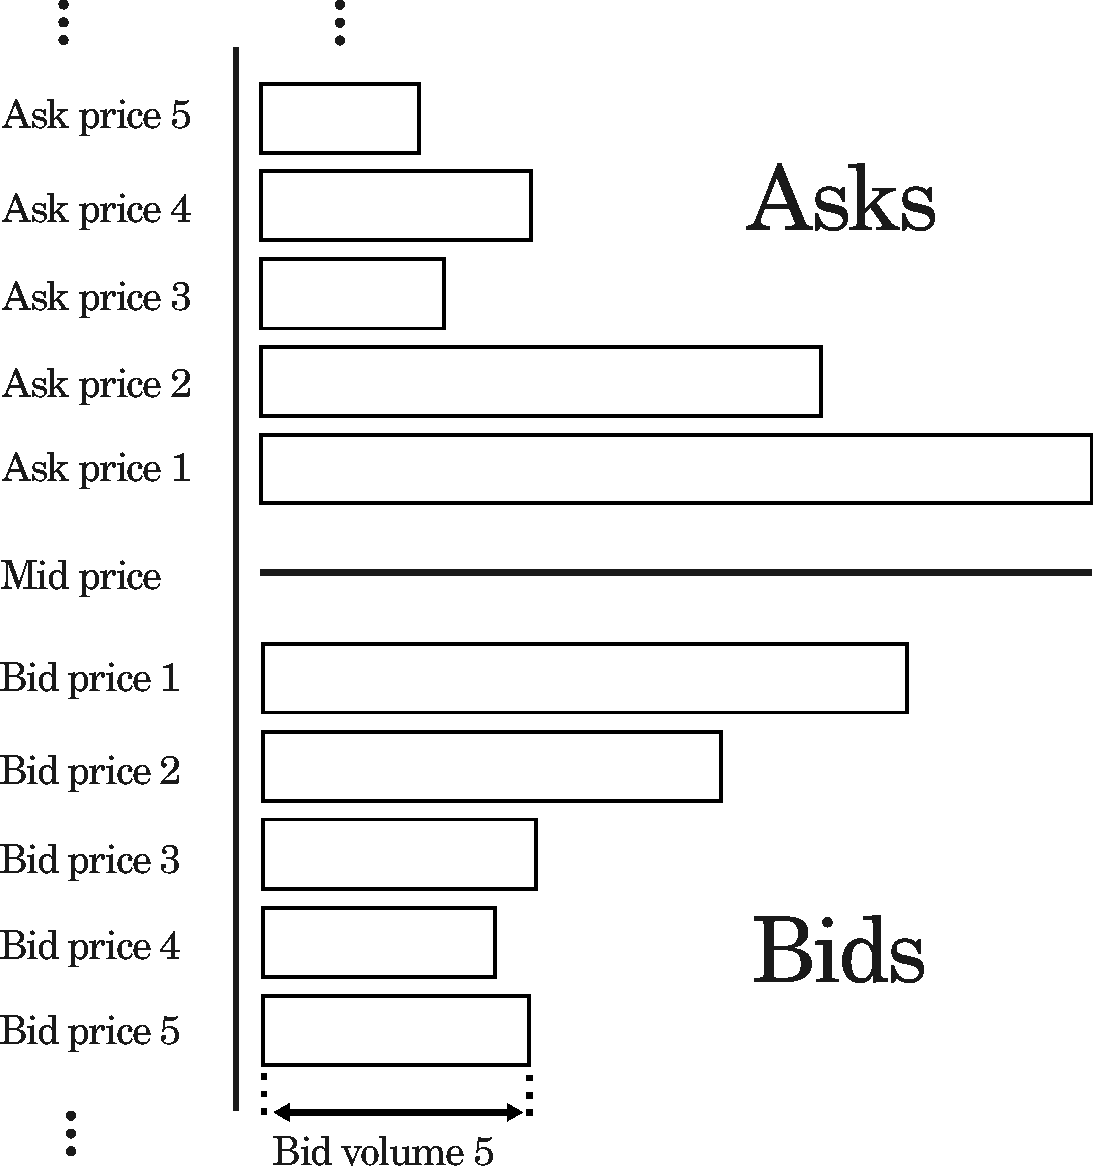
\includegraphics[width=0.5\textwidth]{./images/orderbook.pdf}
    \caption{A visual representation of the orderbook (specifically for L2 data).}
    \label{fig:orderbook}
\end{figure}

It is important to note that there are three main levels of granularity 
when it comes to orderbook representations.
Firstly we have L1 data, which is only the best bids and asks, with their corresponding volumes.
Then we have L2 data, which is all price levels with their corresponding volumes, with one volume value
per price level (i.e. volumes are summed across orders for each price level). Then the most granular is L3 data,
which contains all price levels, with multiple volume values for each price level. Specifically the volumes at a given price
level are broken down into their individual order values. So if, from time $t-1$ to time $t$, 2 orders
are submitted with volumes $v_a$ and $v_b$, then the $L2$ representation would show $V_t = V_{t-1} + v_a + v_b$,
whereas the L3 representation would give us  $\bm{V_t} = [\bm{V_{t-1}}; v_a, v_b]$

For a more in-depth exposition of the mechanism of the limit orderbook, we refer the interested reader to \cite{MARTIN2013}.


\section{The Data}
In this section we introduce our data source and give some visualizations.

\subsection{Data Source}

Our data has been gathered from Binance directly.
Binance is the largest cryptocurrency exchange in terms of daily volume, with a revenue of \$12 billion in 2022 according to \cite{TULLY2023}. 
It was founded in 2017 by Changpeng Zhao. %Binance was initially based in China, then moved to Japan shortly before the Chinese government restricted cryptocurrency companies. Binance then left Japan for Malta and currently has no official company headquarters. 
Binance was chosen because of its high volume, popularity and decent API availability.
Binance also offers perpetual USDT futures which is the main security of focus for this paper.

\subsection{Websocket Data}
Most communication on the internet takes place via a communication protocal known as HTTP, or 
Hypertext Transfer Protocol, \cite{HTTP1999}.
HTTP works in a single direction. We send a request to a server, then the server sends back a response
and then the connection is closed.
Of course for real time streaming applications this is too slow and ideally we would like to keep
the connection open continuously. Introducing the WebSocket protocol, \cite{WEBSOCKET2011}.
WebSocket is a bidirectional communication protocol that can send data from a client to a server
or from a server to a client by reusing the established connection channel.
The connection is kept open until terminated by either the server or the client.
Almost all live streaming applications such as trading, monitoring, etc. use the
WebSocket protocol to continuously receive the live data on a single communication channel.

Binance offers live Websocket data with various endpoints. 
We use the endpoint: 

\url{wss://fstream.binance.com/ws/{trading pair}@depth{L}@100ms}

to stream top L best bids and asks every approximately 100ms.
We log this data to an SQL database on an AWS server.
Due to free-tier limitations we only have about 30GB of storage on the server,
which corresponds to approximately a month of data for four trading pairs. 
This is also about the limit of how much data we can fit into memory at any one time. For these reasons
we only work with 20 days of data, from the start to the end of February, 2024. Specifically
we have data for 2024-02-05 13:07:53.664 until 2024-02-25 11:18:50.866.
This gives us approx. 12 million datapoints for each trading pair.
Since we are looking at such high frequencies, this data should be satisfactory.
We choose BTCUSDT, ETHUSDT, SOLUSDT and MATICUSDT as our futures trading pairs of interest. We choose
these because they are all high enough volume to have good liquidity but also have significant
enough difference in traded volume so that their comparative study should be interesting.
We store this data as a DataFrame for each trading pair. Each row contains the top 10 bid and ask prices and quantities
for a given time. See Table \ref{table:websocket} for an example DataFrame for MATICUSDT. 

\begin{table}[ht]
\centering
\resizebox{0.99\textwidth}{!}{
    \begin{tabular}{llllllllllllll}
    \toprule
    Row & timestamp & ask\_price\_1 & ... & ask\_price\_10 & bid\_price\_1 & ... & bid\_price\_10 & ask\_qty\_1 & ... & ask\_qty\_10 & bid\_qty\_1 & ... & bid\_qty\_10 \\
    \midrule
    0 & 1707138494390 & 0.7877 & ... & 0.7886 & 0.7876 & ... & 0.7867 & 9368.0 & ... & 58006.0 & 15095.0 & ... & 44990.0 \\
    1 & 1707138494515 & 0.7877 & ... & 0.7886 & 0.7876 & ... & 0.7867 & 9367.0 & ... & 58006.0 & 15095.0 & ... & 84785.0 \\
    2 & 1707138494760 & 0.7877 & ... & 0.7886 & 0.7876 & ... & 0.7867 & 9367.0 & ... & 58006.0 & 15095.0 & ... & 44990.0 \\
    3 & 1707138494881 & 0.7877 & ... & 0.7886 & 0.7876 & ... & 0.7867 & 9367.0 & ... & 58006.0 & 15095.0 & ... & 44990.0 \\
    4 & 1707138495248 & 0.7877 & ... & 0.7886 & 0.7876 & ... & 0.7867 & 9356.0 & ... & 58006.0 & 15099.0 & ... & 44990.0 \\
    \vdots & \vdots & \vdots & \vdots & \vdots & \vdots & \vdots & \vdots & \vdots & \vdots & \vdots & \vdots & \vdots & \vdots \\
    11294483 & 1708857980137 & 0.9726 & ... & 0.9735 & 0.9725 & ... & 0.9716 & 16199.0 & ... & 64495.0 & 20555.0 & ... & 37554.0 \\
    11294484 & 1708857980246 & 0.9726 & ... & 0.9735 & 0.9725 & ... & 0.9716 & 16199.0 & ... & 61163.0 & 19527.0 & ... & 37554.0 \\
    11294485 & 1708857980360 & 0.9726 & ... & 0.9735 & 0.9725 & ... & 0.9716 & 20199.0 & ... & 61163.0 & 19527.0 & ... & 37554.0 \\
    11294486 & 1708857980494 & 0.9726 & ... & 0.9735 & 0.9725 & ... & 0.9716 & 21610.0 & ... & 61163.0 & 19577.0 & ... & 37554.0 \\
    11294487 & 1708857980602 & 0.9726 & ... & 0.9735 & 0.9725 & ... & 0.9716 & 22992.0 & ... & 61163.0 & 18401.0 & ... & 37554.0 \\
    \bottomrule
    \end{tabular}
}
\caption{Example data for MATICUSDT.}
\label{table:websocket}
\end{table}

We note that the websocket data is not regular, but comes \textbf{approximately} every 100ms.
This means that the time difference/timedelta, $\Delta t$ ms between updates is not constant and therefore this is technically not
a timeseries in the proper sense. For some of our applications we will resample this data into regular intervals.
We present summary statistics for the timedeltas for each symbol in table \ref{timedelta_table}. We see that most of
the timedeltas are larger than the 100ms promised by the endpoint, with a mean of 133ms and median 116ms.
We also see a maximum timedelta of around 1 minute and a minimum timedelta of 3ms. Whilst this is less than
ideal for an experimental setup, we leave these outliers in, since they represent the real world inconsistencies that
one would find when using such a data source.

\begin{table}[ht]

\resizebox{\textwidth}{!}{
    \begin{tabular}{lrrrr}
    \toprule
     & BTCUSDT $\Delta t$ ms & ETHUSDT $\Delta t$ ms & MATICUSDT $\Delta t$ ms & SOLUSDT $\Delta t$ ms \\
    \midrule
    count & 12891080 & 13612890 & 11294487 & 13334051 \\
    median & 116 & 114 & 122 & 115 \\
    mean & 133 & 126 & 152 & 129 \\
    std & 50& 41& 82& 47\\
    min & 3 & 3 & 3 & 3 \\
    25\% & 107 & 105 & 108 & 107 \\
    50\% & 116 & 114 & 122 & 115 \\
    75\% & 142 & 133 & 162 & 135 \\
    max & 61604 & 61862 & 61697 & 61815 \\
    \bottomrule
    \end{tabular}
}

\caption{Summary statistics for the time difference between observations in our dataset in ms, $\Delta t$ ms, for each trading pair.}
\label{timedelta_table}
\end{table}

\begin{figure}[ht]
    \centering
    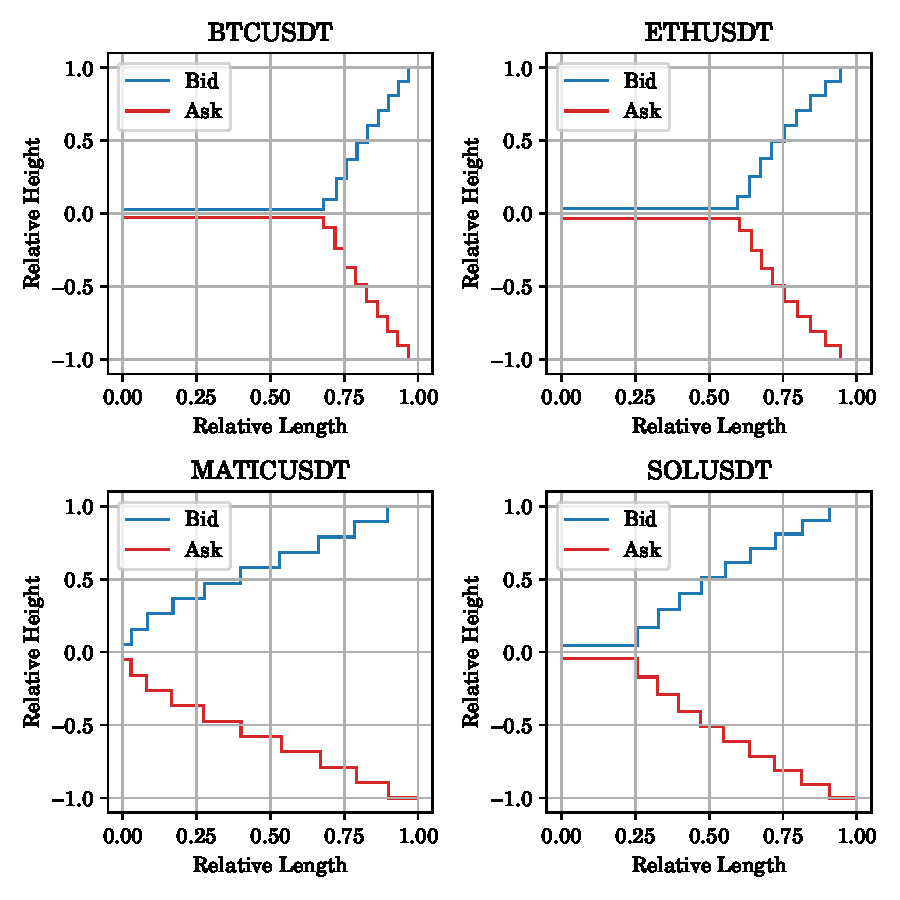
\includegraphics[width=0.99\textwidth]{./images/shapes.pdf}
    \caption{Average orderbook shape for each trading pair.}
    \label{shape}
\end{figure}

\clearpage

\section{Orderbook Shape}

In this section we aim to give a general overview of the shape of the orderbook for each trading pair in our data.
We define the height of a level $\ell \in \{ 1, 2, \dots, 10 \}$ on the $x$ side as $\Delta p_{\ell}^x = p_{\ell}^x - p_{\ell-1}^x$, with $x \in{\{ B,A \}}$. 
Where $B,A$ denote the bid, ask sides respectively. 
In other words, the price difference between the $\ell^{th}$ and $\ell-1^{th}$ bid/ask price level.
We note that by definition, $\Delta p_{\ell}^A < 0, ~ ~ \forall \ell$ and $\Delta p_{\ell}^B > 0, ~ ~ \forall \ell$.
The length of a level $\ell$ on the $x$ side is denoted by $q^x_{\ell}$ and represents the total volume
for the $\ell^{th}$ price level.
We also define the mid-price as an average of the best bid and ask price, i.e.
\begin{equation}
    p_0 := \frac{1}{2} (p^A_{1} + p^B_{1}) \label{mid}
\end{equation}
Following \cite{CAO2009}, we normalize the level heights by the price difference
between the 10th level and the mid-price, i.e. total height. 
The level length is also normalized by the total length from the first level to the 10th level, i.e.
\begin{align}
    \tilde{q}_{l}^x &:= \frac{q_{l}^x}{\sum_{j=1}^{10} q_{j}^x}  \\
    \Delta\tilde{p}_{l}^x &:= \frac{\Delta p_{l}^x}{\sum_{j=1}^{10} \Delta p_{j}^x} = \frac{\Delta p_{l}^x}{|p_{0} - p_{10}^x|}
\end{align}

We average the bids and asks over all entries and then calculate the normalized lengths
and heights. We visualize the results for each trading pair in Figure \ref{shape}.
This gives us a good idea of the overall average shape of the orderbooks.

We see that across all trading pairs the average orderbook is mostly symmetric,
which is what we would expect. Perhaps more interestingly we see that for BTCUSDT the relative
length for the first price level is much larger (higher volume) compared to the other top 10 levels.
In fact, we observe that the relative length of the first level seems to be increasing as a function
of the trading pairs popularity/volume. If we were to order the trading pairs in terms of trading volume, from 
lowest to highest we would have MATICUSDT, SOLUSDT, ETHUSDT and BTCUSDT. This ordering
is also the ordering of the relative length of the first level. So it seems that
the more popular a trading pair is, the more the volume is weighted towards the top of
the orderbook. Also another interesting point is that after the first level
the relative lengths are almost identical, suggesting e.g. that there is just as much
activity in the 10th level compared to the 2nd level of the orderbooks.
\cite{CAO2009} used a similar methodology to visualize the shape of the orderbook,
but for stocks from the Australian Securities Exchange, ASX. The shape of the orderbook
found in \cite{CAO2009} looks a lot like the MATICUSDT orderbook shape, which
agrees with our previously discussed first level length - volume relationship, since the ASX
(in 2009) had much less volume compared to BTCUSDT in 2024.

\section{Orderflow Imbalance}
In this section we introduce a key concept in this paper, \textit{orderflow}, which was first introduced in
\cite{CONT2013}, in the context of linear price impact modelling. We take a brief detour
here to apply this model to our data, in order to motivate the use of orderflow later on in our predictive modelling.

We start by defining the Orderflow Imbalance, a stationary transformation of the orderbook data
first introduced in \cite{CONT2013}.
Since mid-price movement is governed by supply and demand, we need to identify
the different orderbook states and how they relate to supply and demand.
We will initially only concern ourselves with the top of the orderbook.

For each of our observations, we have the best bid price and best bid quantity,
which we denote by $p^B, q^B$ and the best ask price and best ask quantity  $p^A, q^A$.
If we enumerate our observations through time by $n$, then according to \cite{CONT2013}, we have
the following orderbook events:
 \begin{itemize}
     \item $p_n^B > p_{n-1}^B$ or  $q_n^B > q_{n-1}^B$, suggesting an increase in demand.
     \item $p_n^B < p_{n-1}^B$ or  $q_n^B < q_{n-1}^B$, suggesting a decrease in demand.
     \item $p_n^A < p_{n-1}^A$ or  $q_n^A > q_{n-1}^A$, suggesting an increase in supply.
     \item $p_n^A > p_{n-1}^A$ or  $q_n^A < q_{n-1}^A$, suggesting a decrease in supply.
\end{itemize}
Then \cite{CONT2013} defines the quantity $e_n$ to represent the contribution of the  $n^{\text{th}}$ event
as $e_n := e_n^B - e_n^A$ where  $e_n^B$ and $e_n^A$ are defined in (\ref{eBeA}).
\begin{equation}
    \begin{aligned}
        e_{n}^B &:= I_{\{ p_{n}^B \geq p_{n-1}^B \}} q_{n}^B  - I_{\{ p_{n}^B \leq p_{n-1}^B \}} q_{n-1}^B \\
        e_{n}^A &:= I_{\{ p_{n}^A \leq p_{n-1}^A \}} q_{n}^A - I_{\{ p_{n}^A \geq p_{n-1}^A \}} q_{n-1}^A
    \end{aligned}
    \label{eBeA}
\end{equation}
% &= (\Delta q_{n}^B I_{\{ \Delta p_{n}^B \leq 0 \}} + q_{n}^B (I_{\{ \Delta p_{n}^B \geq 0 \}}  - I_{\{ \Delta p_{n}^B \leq 0 \}})) - (\Delta q_{n}^A I_{\{ \Delta p_{n}^A \geq 0 \}} + q_{n}^A (I_{\{ \Delta p_{n}^A \leq 0 \}} - I_{\{ \Delta p_{n}^A \geq 0\}})) \label{diff}
% Where (\ref{diff}) allows for efficient computation using the diff operator.
Then we sum these individual contributions from time $t-h$ to the current time $t$,
to get the Order Flow Imbalance at time $t$:
\begin{equation}
    \text{OFI}_h(t) := \sum_{n : t_n \in [t-h, t]} e_n
    \label{OFI}
\end{equation}

\subsection{Linear Price Impact Model}
In this subsection we introduce the linear price impact model from \cite{CONT2013} that motivates
the above orderflow definition.
Firstly, let us define $\Delta p_{\delta}(t+h) := (p(t+h) - p(t)) / \delta$, i.e. the change in price
measured in ticks, where $\delta$ is the ticksize for the given trading pair. Note that a tick
is defined as the smallest price increment in which the price for a pair is quoted, i.e. the precision.
Using the Binance API we
retrieve the ticksizes as:  % TODO: Format this better
\begin{table}[ht]
    \centering
    \begin{tabular}{ll}
        \toprule
        trading pair & $\delta$ \\
        \midrule
        BTCUSDT & 0.1 \\
        ETHUSDT & 0.01 \\
        SOLUSDT & 0.001 \\
        MATICUSDT & 0.0001 \\
        \bottomrule
    \end{tabular}
    \caption{Trading pairs and their ticksizes, $\delta$.}
\end{table}

\cite{CONT2013} considers a stylized model of the orderbook where the volume beyond the top level
is equal to $D$ and all trading activity only occurs at the top level. Of course this is a big
assumption but from our previous exploration we showed this to be largely justified for high volume pairs such
as BTCUSDT and ETHUSDT. Under these assumptions, we have three main events on the bid side:
\begin{enumerate}
    \item Market sell orders remove $M^s$ volume from the bid.
    \item Limit buy orders add $L^b$ volume to the bid.
    \item Limit buy cancels remove $C^b$ volume from the bid.
\end{enumerate}
We can analogously define quantities for the ask side.
Then under the above assumptions:
\begin{equation}
    \Delta p = \left\lceil (L^b - C^b - M^s) / 2D \right\rceil  - \left\lceil (L^s -C^s - M^b) / 2D \right\rceil
\end{equation}

This is equivalent, (up to some truncation) to:
\begin{equation}
    \Delta p = \frac{\text{OFI}}{2D} + \epsilon
\end{equation}
since $\text{OFI} = L^b - C^b-M^s-L^s+C^s+M^b$.

So under our stylized assumptions, we see that the price change in ticks
is directly proportional to the Orderflow Imbalance.
Therefore \cite{CONT2013} suggest the following relation:
\begin{equation}
    \Delta p_{\delta}(t) = \beta \text{OFI}_h(t) + \epsilon_t \label{linearrelation}
\end{equation}
where $\beta$ is the \textit{price impact coefficient} and $\epsilon_t$ is the noise
term. So $\beta$ measures the instantaneous impact of the $n^{th}$ event on the mid-price. 
\cite{CONT2013} assume the price impact coefficients are constant for half-hour intervals (indexed by $i$),
and estimate them using OLS:
\begin{equation}
    \Delta p_{\delta}(t) = \hat{\beta}_i \text{OFI}_h(t) + \hat{\alpha}_i + \hat{\epsilon}_t
\end{equation}

\subsection{PanelOLS Results}
We split our data into half-hour windows and then perform PanelOLS across windows
to estimate the average coefficients. We set $h = 1000ms$ and present the results for
BTCUSDT here. (The $R^2$ values for the other symbols are very similar and can be found in the appendix).

\begin{table}[H]
\textbf{BTCUSDT PanelOLS Results for h = 1000ms}
\begin{center}
\begin{tabular}{lclc}
\hline
\textbf{Dep. Variable:}    &         $\Delta p_{\delta}$         & \textbf{  R-squared:         }   &      0.3590      \\
\textbf{Estimator:}        &      PanelOLS      & \textbf{  R-squared (Between):}  &     -0.3865      \\
\textbf{No. Observations:} &      12891080      & \textbf{  R-squared (Within):}   &      0.3590      \\
\textbf{Date:}             &  Tue, Mar 26 2024  & \textbf{  R-squared (Overall):}  &      0.3585      \\
\textbf{Time:}             &      16:15:04      & \textbf{  Log-likelihood     }   &    -6.11e+07     \\
\textbf{Cov. Estimator:}   &     Clustered      & \textbf{                     }   &                  \\
\textbf{}                  &                    & \textbf{  F-statistic:       }   &    7.218e+06     \\
\textbf{Entities:}         &        956         & \textbf{  P-value            }   &      0.0000      \\
\textbf{Avg Obs:}          &     1.348e+04      & \textbf{  Distribution:      }   &  F(1,12890123)   \\
\textbf{Min Obs:}          &       953.00       & \textbf{                     }   &                  \\
\textbf{Max Obs:}          &     1.676e+04      & \textbf{  F-statistic (robust):} &      4743.2      \\
\textbf{}                  &                    & \textbf{  P-value            }   &      0.0000      \\
\textbf{Time periods:}     &       16761        & \textbf{  Distribution:      }   &  F(1,12890123)   \\
\textbf{Avg Obs:}          &       769.11       & \textbf{                     }   &                  \\
\textbf{Min Obs:}          &       1.0000       & \textbf{                     }   &                  \\
\textbf{Max Obs:}          &       956.00       & \textbf{                     }   &                  \\
\textbf{}                  &                    & \textbf{                     }   &                  \\
\hline
\end{tabular}
\begin{tabular}{lcccccc}
             & \textbf{Parameter} & \textbf{Std. Err.} & \textbf{T-stat} & \textbf{P-value} & \textbf{Lower CI} & \textbf{Upper CI}  \\
\hline
\textbf{OFI} &       1.1829       &       0.0172       &      68.871     &      0.0000      &       1.1492      &       1.2166       \\
\hline
\end{tabular}
%\caption{PanelOLS Estimation Summary}
\end{center}
F-test for Poolability: 19.309, \\
Distribution: F(955,12890123),\\
Included effects: Entity.
\end{table}

\begin{figure}[H]
    \centering
    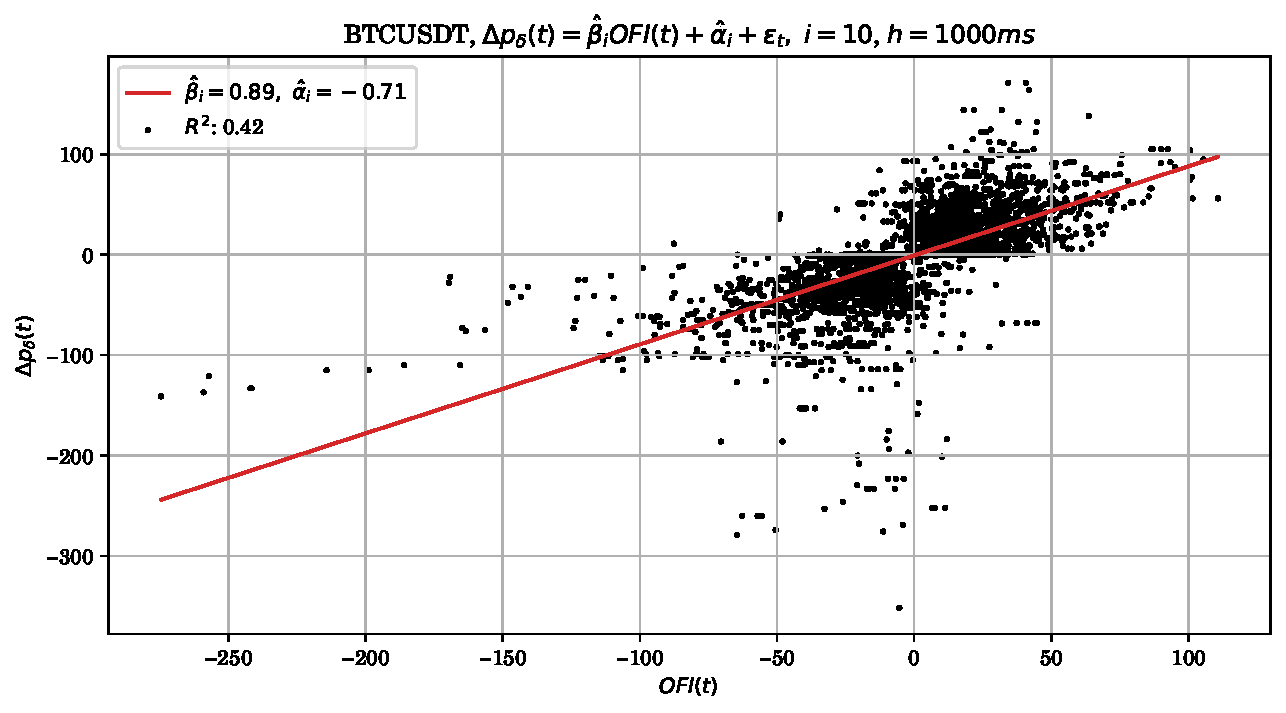
\includegraphics[width=0.8\textwidth]{./images/btcusdt_h=1000ms_contemp_OFI.pdf}
    \caption{OFI contemporaneous regression for an example half-hour window for BTCUSDT.}
    \label{fig:contemp_OFI_btcusdt}
\end{figure}

We observe very similar $R^2$ values across all trading pairs, around $0.35$, confirming the
linear relation (\ref{linearrelation}). We also visualize the regression for an example half hour window in Figure \ref{fig:contemp_OFI_btcusdt}.
% Interestingly we see that the $\Delta p_{\delta}(t)$ values for MATICUSDT
% are far more sparse than the other trading pairs, with fewer unique values, and much more clearly
% defined steps. This is much more similar to the results of \cite{CONT2013} and 
% perhaps is characteristic of securities with lower volume.

We repeat the procedure for different values of $h$ and plot the results in Figure \ref{r2_h}.
We see that $R^2$ increases in  $h$ and then plateaus around $h=20,000ms$.

Instead of averaging across intervals, we can also examine how the price impact coefficients change
across intervals. We visualize the results in Figures \ref{fig:BTCUSDT_beta_across_time} - \ref{fig:MATICUSDT_beta_across_time}.
We see that, for our data, for all trading pairs the average price impact coefficient is initially decreasing in time
for the first few hours of the day. It then recovers and begins to (roughly) increase again.
We also see that the variance of the price impact coefficients are fairly constant across different intervals.
The fact that we have trends in price impact coefficients suggests that
the impact of a new orderbook event on the mid-price varies throughout the day, with
some periods having less impact (assuming the linear price impact model given by (\ref{linearrelation})).
The smallest average coefficients seem to occur around 06:00AM and so we suggest placing trades around this time
if the goal is to minimize price impact.

\subsection{Conclusion}
Whether this model is too simple to realistically model price impact in a useful way is not something we explore in this paper.
The purpose of this section rather, was to introduce orderflow and show that it has relevance for influencing price changes in the orderbook.


\begin{figure*}[htpb]
   \centering
   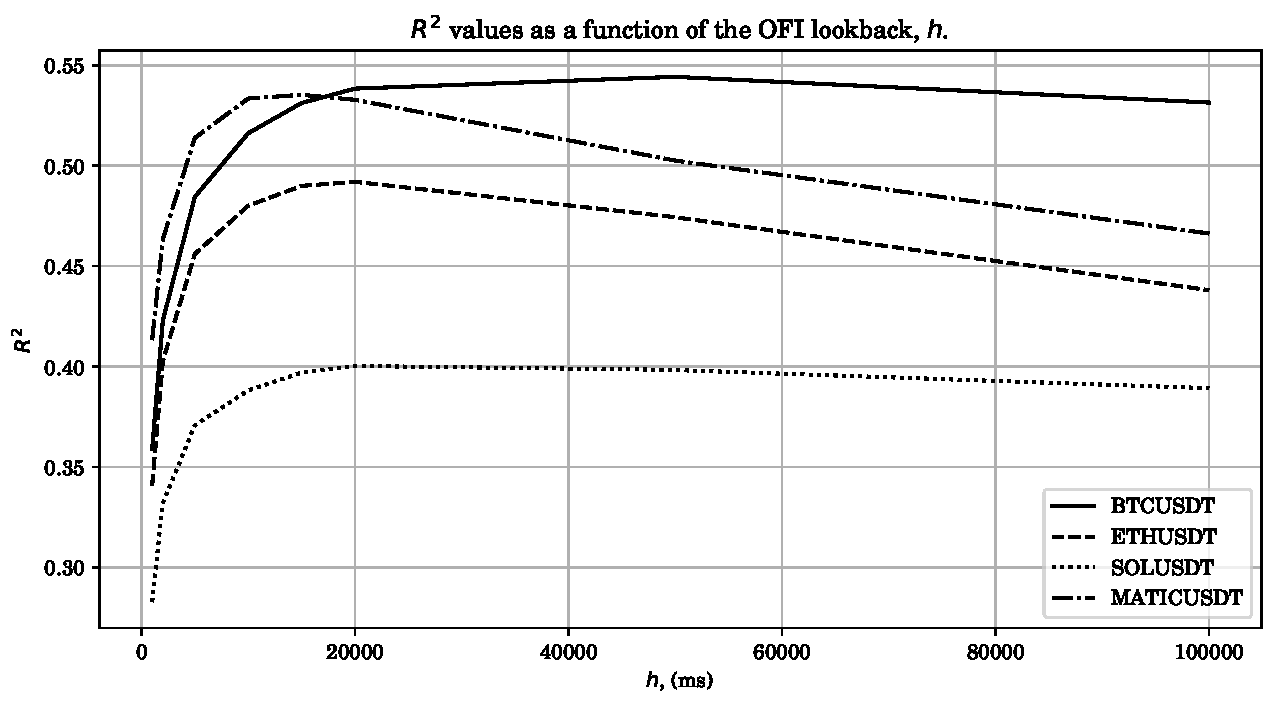
\includegraphics[width=1.0\textwidth]{./images/OFI_r2_h.pdf}
   \caption{Effect on contemporaneous regression $\Delta p_{\delta}(t) = \hat{\beta}_i \text{OFI}_h(t) + \hat{\alpha}_i + \hat{\epsilon}_t$,
       $R^2$ values when varying the lookback period, $h$, that defines $\text{OFI}_h(t)$.
    }
   \label{r2_h}
\end{figure*}

\clearpage

\begin{figure*}[htpb]
    \centering
    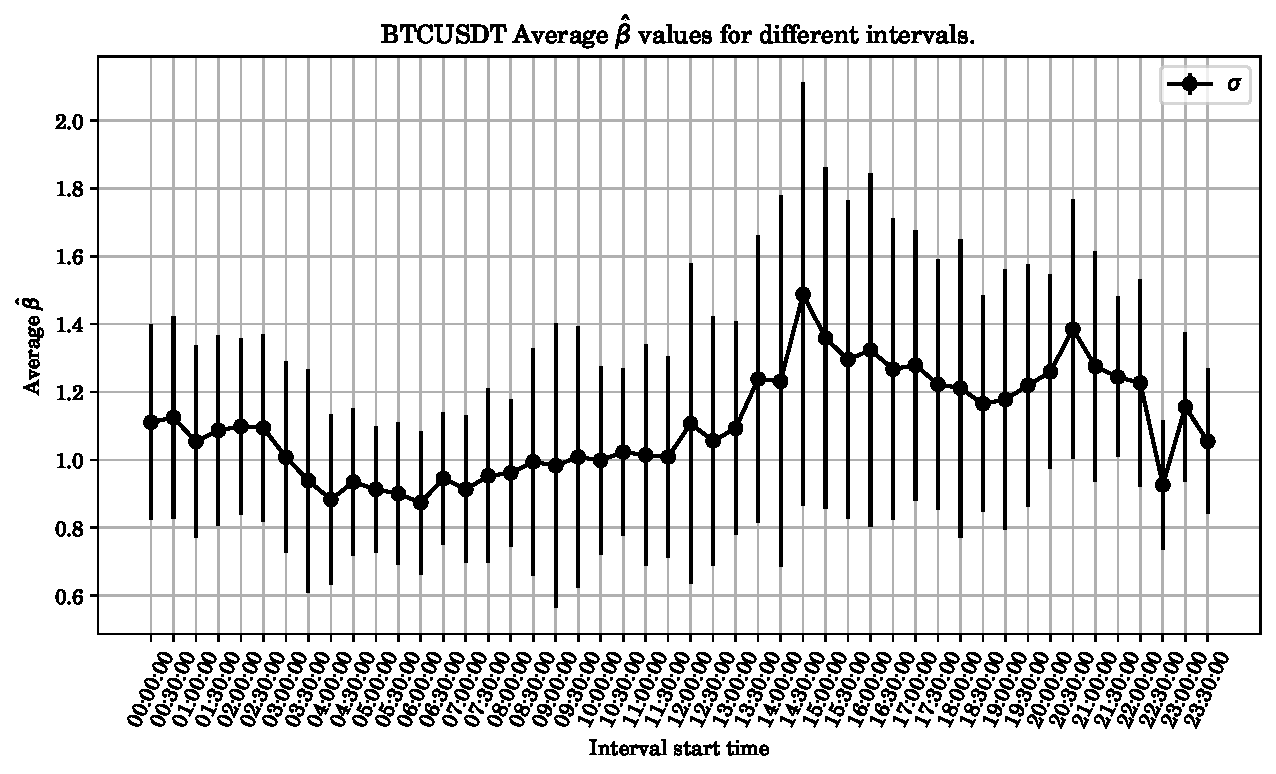
\includegraphics[width=0.8\textwidth]{./images/BTCUSDT_beta_across_time.pdf}
    \caption{BTCUSDT Average price impact coefficients for different half-hour intervals. Note that errorbars represent standard deviations.}
    \label{fig:BTCUSDT_beta_across_time}
\end{figure*}


\begin{figure*}[htpb]
    \centering
    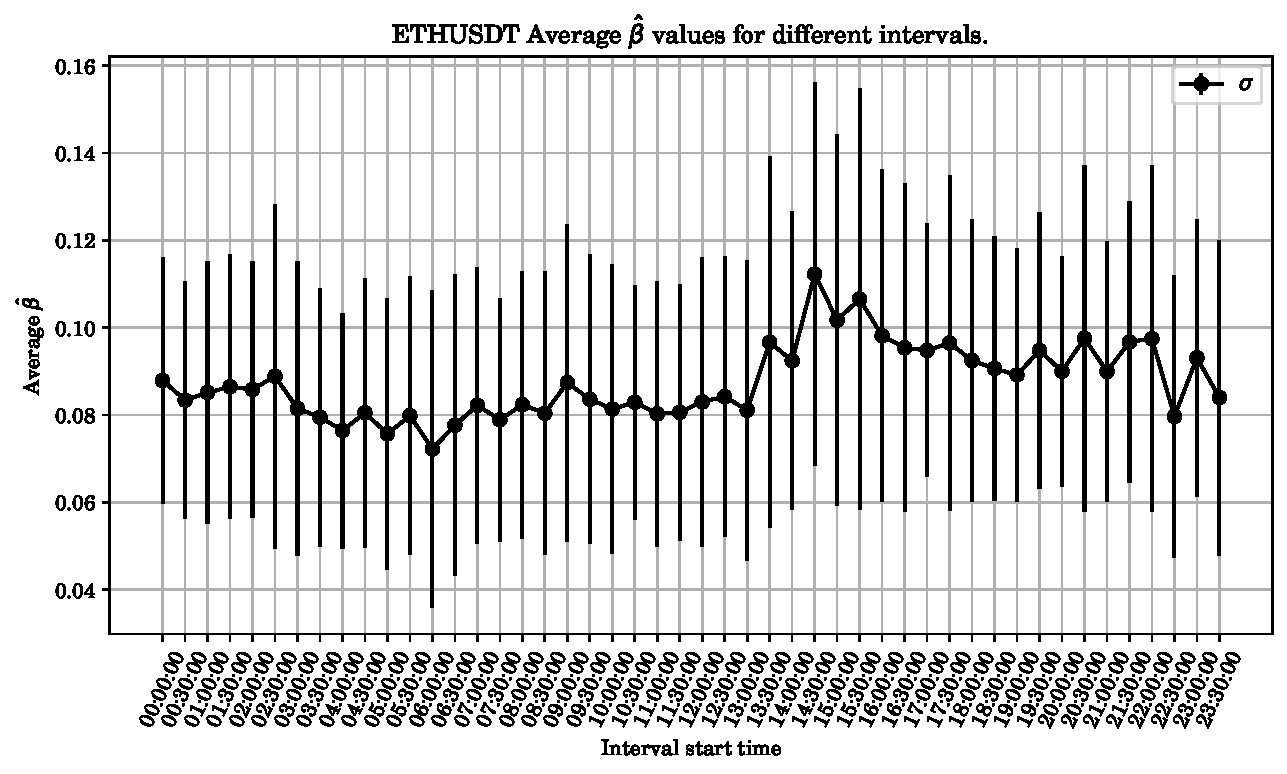
\includegraphics[width=0.8\textwidth]{./images/ETHUSDT_beta_across_time.pdf}
    \caption{ETHUSDT Average price impact coefficients for different half-hour intervals. Note that errorbars represent standard deviations.}
\end{figure*}

\begin{figure*}[htpb]
    \centering
    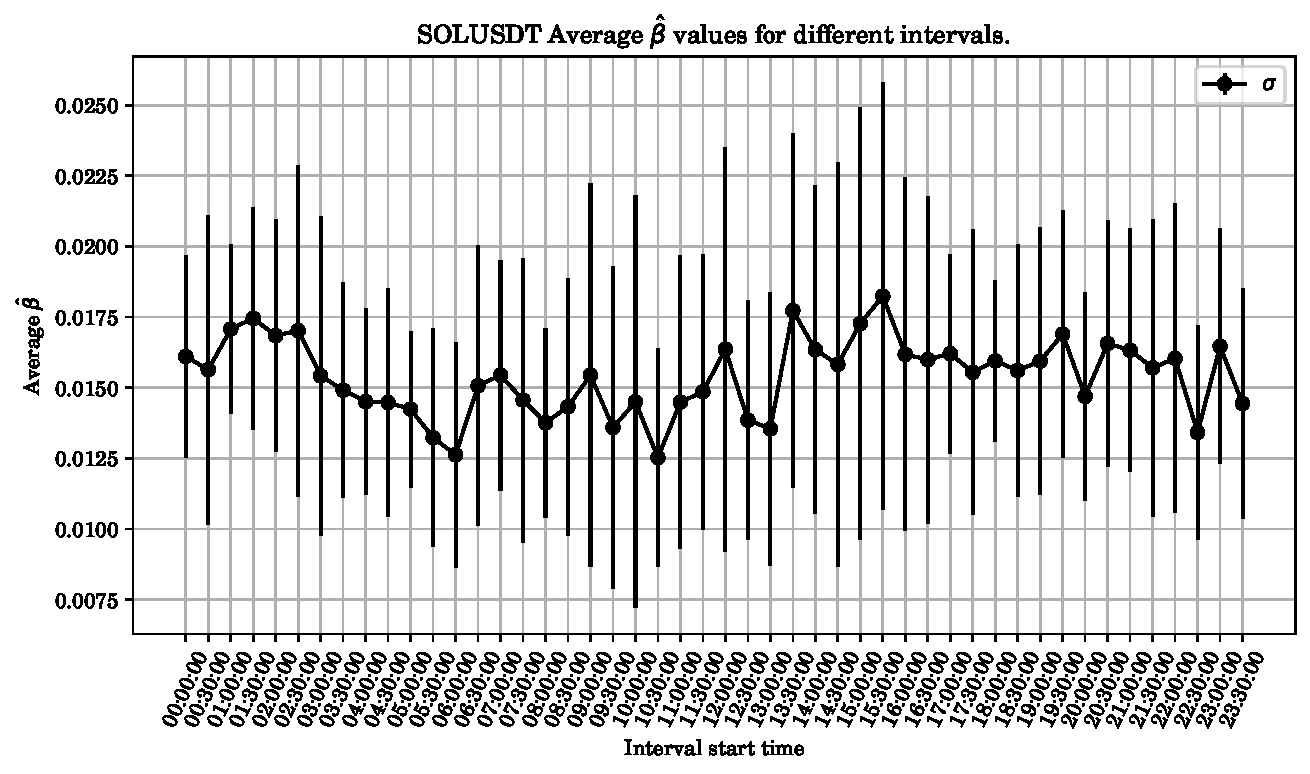
\includegraphics[width=0.8\textwidth]{./images/SOLUSDT_beta_across_time.pdf}
    \caption{SOLUSDT Average price impact coefficients for different half-hour intervals. Note that errorbars represent standard deviations.}
\end{figure*}

\begin{figure*}[htpb]
    \centering
    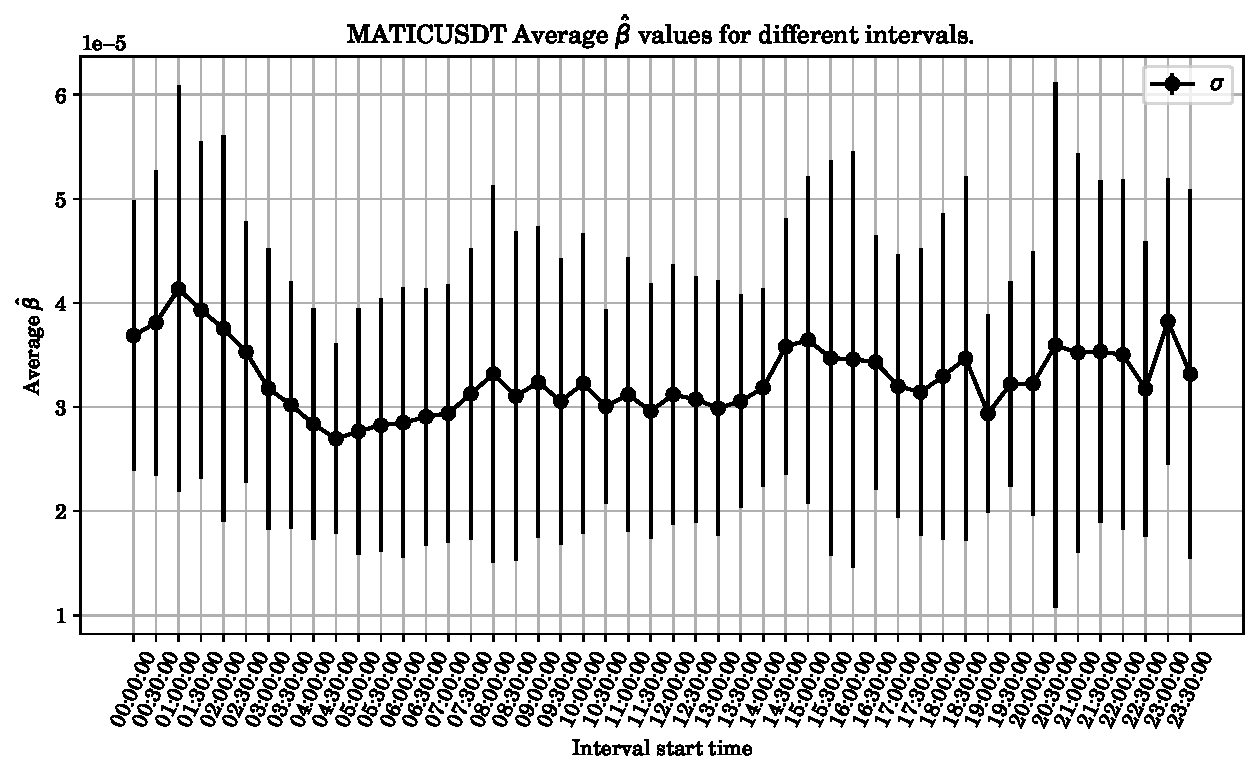
\includegraphics[width=0.8\textwidth]{./images/MATICUSDT_beta_across_time.pdf}
    \caption{MATICUSDT Average price impact coefficients for different half-hour intervals. Note that errorbars represent standard deviations.}
    \label{fig:MATICUSDT_beta_across_time}
\end{figure*}



\chapter{Predictive Modelling}
\hrule
\vspace{40pt}


\section{The Modelling Objective}

Our main aim in this chapter is to predict future mid-price\footnote{Recall in (\ref{mid}) we defined the mid-price, $p_0(t)$ to be the average of the best bid and ask prices at time $t$.}
movement. 
There are multiple possible modelling setups when it comes to mid-price movement prediction.
\cite{KOLM2023} frame this as a regression problem, directly predicting future mid-price values at multiple horizons.
\cite{ZHANG2019} and \cite{LUCCHESE2024} predict the sign of the returns, in a multi-class classification setting.
They argue that due to the highly stochastic nature of financial data, simply calculating labels based on returns from $p_{0}(t)$ and $p_{0}(t+k)$ 
leads to a label set with a lower signal to noise ratio, so smoothed returns are used.

In this paper we use the multi-class classification setup.
Following \cite{ZHANG2019}, we adopt the smoothed labelling method first introduced in \cite{AVRAAM2017}. Define the quantites:
\begin{align}
    m_{-}(t) &:= \frac{1}{k} \sum_{i=0}^{k} p_0(t-i) \\
    m_{+}(t) &:= \frac{1}{k} \sum_{i=1}^{k} p_0(t+i) \\
    \ell(t) &:= \frac{m_{+}(t) - m_{-}(t)}{m_{-}(t)}
    \label{smoothed_returns}
\end{align}
So $m_{-}(t)$ represents the average price for the previous $k$ prices and current price
and $m_{+}(t)$ represents the average price for the next $k$ prices.
Then we calculate the smoothed returns $\ell(t)$ as the return of this smoothed price. 
Then we discretize these returns according to (\ref{desc}) in order to give us three distinct class labels for use in classification.

\begin{equation}
    y(t) = \begin{cases} \label{desc}
        +1  & \text{ if } \ell(t) \in (\epsilon, \infty) \\
        0  & \text{ if } \ell(t) \in [-\epsilon, \epsilon] \\
       -1  & \text{ if } \ell(t) \in  (-\infty, -\epsilon)
   \end{cases}
\end{equation}
So given the information we have up to and including time $t$, our aim is to build a model to predict $y(t)$.

See Figure \ref{fig:example_mid_price_labelling} for a sample of our mid-price data,
colour coded according to class label. We see regions of mid-price downtrend are labelled
with -1 (coloured red), regions of mid-price plateau are labelled with 0 (coloured blue)
and regions of mid-price uptrend are labelled with +1 (coloured green).

\begin{figure}[ht]
    \centering
    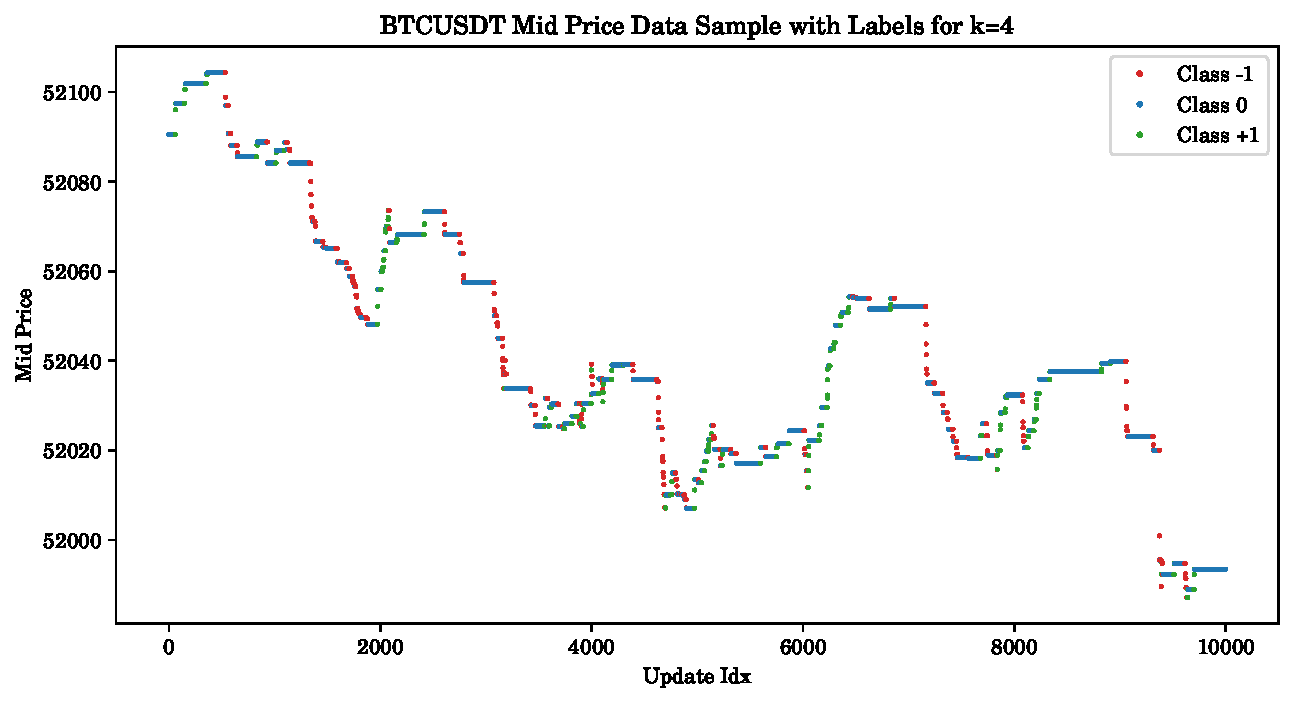
\includegraphics[width=1.0\textwidth]{./images/example_labels.pdf}
    \caption{An example BTCUSDT mid-price sample, coloured according to class label.
    Note that the discretization parameter, $\epsilon$ is set $\approx 0$ and the prediction horizon is $k=4$ updates.}
    \label{fig:example_mid_price_labelling}
\end{figure}


Note that in some implementations, the prediction horizon is
given over some time interval, such as predicting the movement for the next 10 seconds.
In this paper, we instead define our prediction horizon in terms of ticks/updates/datapoints.
This choice was made as our WebSocket data arrives at irregular times, and for some short intervals
there is no available data. We expect the results to be very similar when using a time-based horizon.


\section{Model Architecture Background}
In this section we explain the general theory needed for our classification models.

\subsection{Logistic Regression}
Linear regression is one of the oldest and most robust predictive models used in all areas
of science. Its simplicity, explainablity and robustness means it is a common choice for a baseline/benchmark
model.

Logistic regression, first introduced in \cite{COX1958}, is the natural extension of linear regression to the classification setting.
The key idea is to model the \textit{log odds} as linear functions of our data.
Suppose we have $C$ classes, indexed by $1, 2, \cdots, C$, then we assume the following linear model: 
\begin{align*}
    \log \frac{\mathbb{P}(Y=1 | X = x)}{\mathbb{P}(Y=C | X = x)} &= \alpha_1 + \beta_1' x \\
   \log \frac{\mathbb{P}(Y=2 | X = x)}{\mathbb{P}(Y=C | X = x)} &= \alpha_2 + \beta_2' x \\
   \vdots \\
   \log \frac{\mathbb{P}(Y=C-1 | X = x)}{\mathbb{P}(Y=C | X = x)} &= \alpha_{C-1} + \beta_{C-1}' x
\end{align*}
Note that because the probabilities must sum to $1$, we have $C-1$ degrees of freedom.
Also note that the choice of denominator is not important as the model is equivariant
under the choice of denominator class.

With some re-arrangement, we get the posterior probabilities:
\begin{align*}
    \mathbb{P}(Y=c | X = x) &= \frac{\exp(\alpha_c + \beta_c' x)}{1 + \sum_{\ell=1}^{C-1} \exp(\alpha_{\ell} + \beta_{\ell}'x)} \\
    \mathbb{P}(Y=C | X = x) &= \frac{1}{1 + \sum_{\ell=1}^{C-1} \exp(\alpha_{\ell} + \beta_{\ell}'x)}
\end{align*}
Where  $c \in {1, 2, \cdots, C-1}.$

Interestingly we note that the log odds representation is equivalent to a bijective mapping of the linear functions $\alpha_c + \beta_c'x$ onto $[0, 1]$ using
the sigmoid function: $1 / 1 + \sigma(-x)$.
Note that the parameters $(\alpha_c, \beta_c)_{c=1}^C$ are fit by maximizing the log-likelihood using gradient descent methods.
So given some observation, $\bm{x}_t$, our model gives us the posterior probabilities of the observation
belonging to each class. In order to make a classification, we can simply choose the class with the highest
posterior probability, and assign this class to $\hat{y}_t$.
We refer the interested reader to \cite{HASTIE2001} for a more in-depth exposition of the theory.

\subsection{Decision Trees}
\textit{Decision Trees} are another very popular class of machine learning models with a
large amount of success in a wide range of fields. There are two main types; decision trees
for classification and decision trees for regression. The theory for both is very similar
and they share the same ideas. We focus on classification here.
The main idea is to learn an \textit{optimal} partition of our data using binary trees,
with each non-leaf node representing a split of our data on one variable.
The model learns which features to split on at each level and which threshold values to use for the splits.
More formally, following \cite{HASTIE2001}, suppose our data is $X \in  \mathbb{R}^{n \times d}$, then
we seek to partition our data into $M$ regions, $R_1, R_2, ..., R_M$, and then our prediction is given by:
\begin{equation}
    \hat{y}(x) = \sum_{m=1}^{M} c_m 1\{x \in  R_m\} 
\end{equation}
Where $c_m$ is the most common class in region $R_m$, i.e.
\begin{equation}
    c_m = \arg \max_{c \{\in {1, 2, ..., C}\}} |\{y_i : y_i = c \land x_i \in R_m\}|
\end{equation}
Consider splitting our data with feature $j$, and threshold $s$. We denote the resulting
partitions with $R_1$ and $R_2$, defined as: 
\begin{equation}
    \begin{aligned}
        R_1(j, s) &:= \{X : X_j \le s\}, \\
        R_2(j, s) &:= \{X : X_j >  s\} 
    \end{aligned}
\end{equation}

The \textit{optimal} $j$ and $s$ are chosen to solve:
\begin{equation}
    j^*, s^* = \arg \min_{j,s}  \mathcal{L}(R_1(j, s), R_2(j, s))
\end{equation}
Where $\mathcal{L}$ is some loss function measuring how well the partition splits the data.

Since checking all combinations of features and threshold values would be computationally infeasible, the fitting
algorithm uses an iterative greedy approach, choosing the optimal splits at each level based on some loss function that
measures how well the split partitions the data for the next level.
One commonly used loss function is the misclassification error:
\begin{equation}
        \mathcal{L}(R_1, R_2) = \min_{c_1} \frac{1}{n_1} \sum_{x_i \in  R_1(j, s)} 1(y_i \neq c_1) + \min_{c_2}\frac{1}{n_2} \sum_{x_i \in  R_2(j, s)} 1(y_i \neq c_2)
\end{equation}
In practice other loss functions, such as \textit{cross-entropy} or \textit{gini impurity}, are often used.
They are also differentiable which is a key property for certain optimization algorithms.
We again refer the interested reader to \cite{HASTIE2001} for a more in-depth discussion of these details.

Simple decision trees have high variance, meaning they can easily overfit to training data.
For this reason, various \textit{ensemble} methods were devised to reduce overfitting.
We introduce one such method, \textit{Boosting}. The basic idea is to iteratively train many \textit{weak learners}
and then combine their predictions to produce a single, more robust prediction. Weak learners are simple models
which are only slightly better than randomly guessing and 
have low variance and high bias. In theory, by combining many weak learners, 
boosting lowers the model bias, whilst keeping variance low.
In more detail, in each iteration, we fit a weak classifier (e.g. a single decision tree stump).
We then compute the error according to some loss function. Then we use this error to define the weight for the current iteration,
then we re-weight our training data, using this weight, so samples where the model performed badly are given more weight in the next iteration.
Then our final output model will be a weighted sum of the predictions of the weak learners.

\begin{figure}[ht]
    \centering
    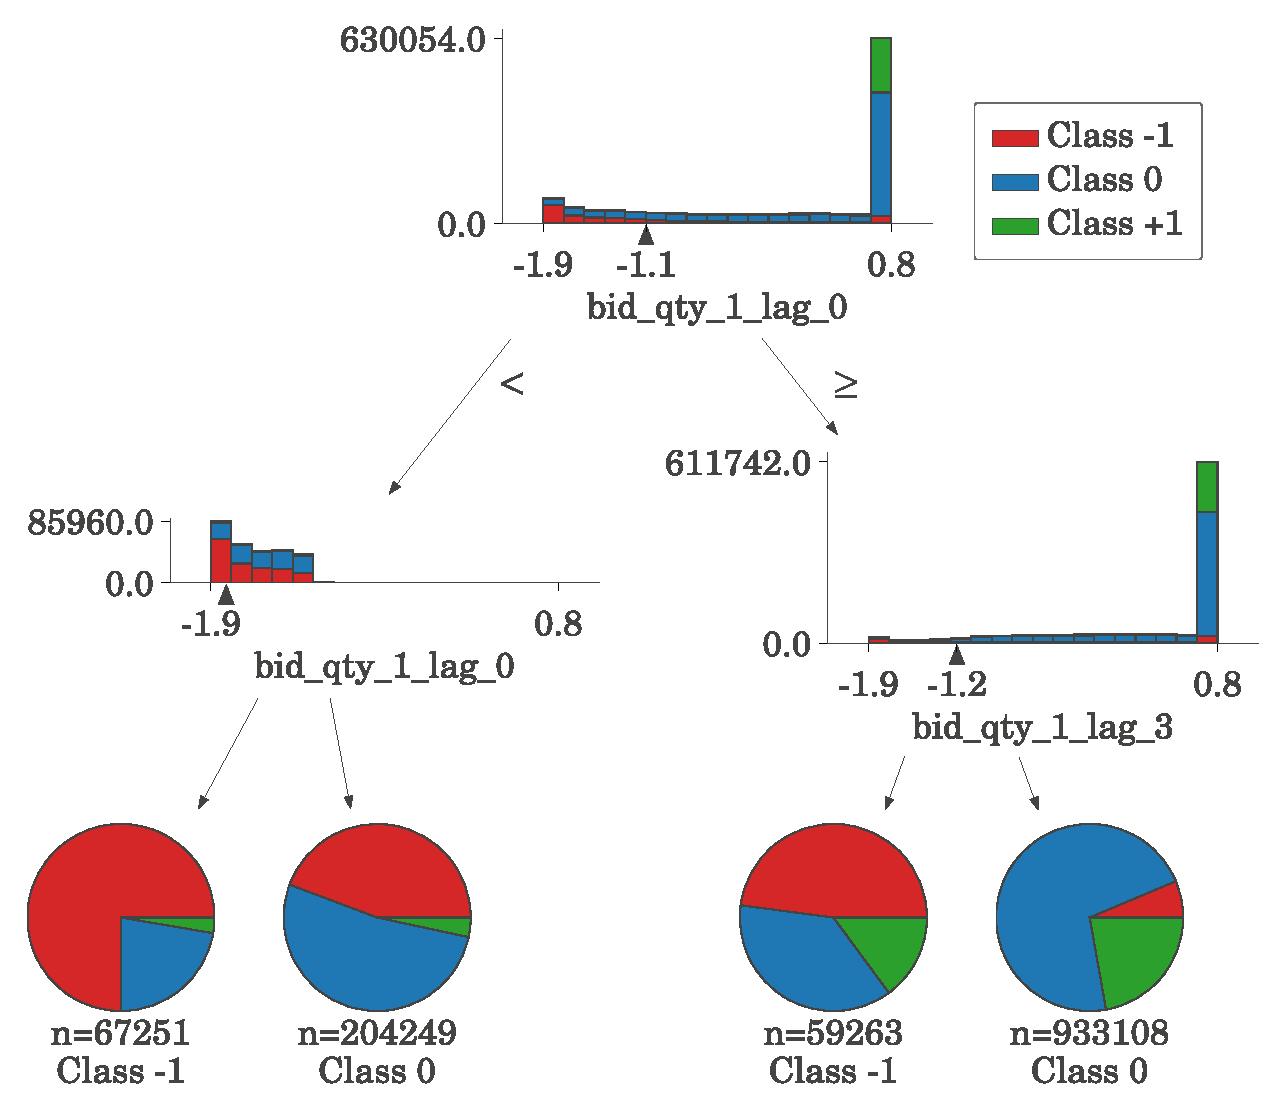
\includegraphics[width=0.7\textwidth]{./images/xgb_viz.pdf}
    \caption{A visualization of a single decision tree weak learner with max depth set to 2.}
    \label{fig:weaklearner}
\end{figure}

\subsection{Artificial Neural Networks}
Artificial Neural Networks are a broad class of machine learning model that can efficiently approximate
high dimensional non-linear functions. Perhaps the most famous example of an ANN (Artifical Neural Network)
is that of the Multi-Layer Perceptron, first introduced in \cite{ROSENBLATT1958}. The basic idea is to take some input
vector and successively project it onto new spaces with affine and then non-linear transformations.
An MLP with $N$ hidden layers can be defined mathematically as:
\begin{equation}
    \begin{aligned}
        f_i(x; W_i, b_i) &= \sigma_i(W_i x + b_i) \\
        f(x; W_1, W_2, ..., W_N, b_1, b_2, ..., b_N) &= f_N \circ f_{N-1} \circ ... \circ f_2 \circ f_1(x)
    \end{aligned}
\end{equation}
Where $W_i$  are learnable weight matrices, $b_i$ are learnable bias vectors, $\sigma_i$ are fixed non-linear activation functions and $\circ$ denotes function composition.
MLPs are powerful because, as \cite{HORNIK1989} shows, they are \textit{universal function approximators}.
This means that, with as few as one hidden layer and using arbitrary activation functions, 
they are capable of approximating any Borel measurable function from one finite dimensional space 
to another to any desired degree of accuracy, provided sufficiently many hidden units are available.
The weight matrices and bias vectors are learnt by minimizing some loss function.
If we denote our learnable parameters as $\theta$, then our loss function is given by:
\begin{equation}
   \mathcal{L} (\theta; x, y) := \frac{1}{n} \sum_{i=1}^{n} \ell(f(x_i; \theta), y_i)
\end{equation}
Where $\ell$ is some observation-wise loss that measures how well our model predicts
$y_i$ given corresponding input $x_i$.
For simple problems $\mathcal{L}$ is commonly a convex function and so gradient descent methods can be
used to perform the minimization. For example, for vanilla gradient descent, one might define the update rule as:
\begin{equation}
    \theta^{(t+1)} \gets \theta^{(t)} - \eta \nabla_\theta \mathcal{L}(\theta^{(t)})
\end{equation}
In practice the optimization problem is often not convex, with many local minima, and so alternative optimization methods
are often used, such as \textit{Stochastic Gradient Descent}, \cite{ROBBINS1951}, or \textit{ADAM}, \cite{ADAM2017}.
Stochastic Gradient Descent is a stochastic approximation of the gradient descent method, that
evaluates the gradient on a randomly sampled subset of the training data, instead of the entire training data.
It can be shown, \cite{ROBBINS1951}, that the stochastic approximation of the gradient converges in expectation to
the gradient evaluated on the entire training dataset.
This sub-sampling allows for fewer gradient evaluations and therefore faster training. Also the stochastic
nature of the algorithm means it is less likely to get stuck in local minima.
ADAM, first introduced in \cite{ADAM2017}, is a more advanced type of Stochastic Gradient Descent
that uses the concept of \textit{Momentum}, \cite{RUMELHART1986}. Momentum accumulates
the gradient from past updates to help guide the direction of the current step. It helps
to reduce oscillations during descent and often leads to faster convergence.

The ADAM update step is given by:
\begin{equation}
    \begin{aligned}
        m_{\theta}^{(t+1)} &\leftarrow \beta _{1}m_{\theta}^{(t)}+\left(1-\beta _{1}\right)\nabla_{\theta} \mathcal{L}(\theta^{(t)}) \\
        v_{\theta}^{(t+1)} &\leftarrow \beta _{2}v_{\theta}^{(t)}+\left(1-\beta _{2}\right)\left(\nabla_{\theta} \mathcal{L}(\theta^{(t)})\right)^{2} \\
        {\hat {m}}_{\theta} &={\frac {m_{\theta}^{(t+1)}}{1-\beta _{1}^{t}}} \\
        {\hat {v}}_{\theta} &={\frac {v_{\theta}^{(t+1)}}{1-\beta _{2}^{t}}} \\
        \theta^{(t+1)} &\leftarrow \theta^{(t)}-\eta {\frac {{\hat {m}}_{\theta}}{{\sqrt {{\hat {v}}_{\theta}}}+\delta }}.
    \end{aligned}
\end{equation}
So we see that ADAM uses exponential moving averages with decay factors $\beta_1$ and $\beta_2$ to accumulate first and
second gradient moments. Note that $\delta$ is some small constant, used to prevent zero division errors.

Using traditional differentiation methods, the $\nabla_\theta \mathcal{L}(\theta^{(t)})$ calculation would be very computationally
expensive and training would be too slow to be practical. Instead, an algorithm called \textit{backpropagation}, \cite{RUMELHART1986},
can be used to efficiently differentiate the network with respect to the weights and biases. 
Backpropagation is an efficient implementation of the chain rule for differentiation that uses
dynamic programming to avoid repeated calculations. The idea is to construct a \textit{computational graph},
which is a graph datastructure, where nodes represent functions and the edges represent function compositions.
So by doing a \textit{forward pass} of the graph, we are essentially evaluating the network given some input.
We then get an output, and do a \textit{backward pass} to accumulate gradients in an efficient way using the chain rule.
Backpropagation has computational complexity of the order of the number of edges in the computational graph,
so for large networks it scales very well and can be made to run extremely efficiently.

\subsection{Convolutional Neural Networks}

Convolutional Neural Networks (CNNs) are a specialized class of artificial neural 
networks designed primarily for processing structured grid data, such as images.
First introduced in \cite{LECUN1998}, CNNs have become a cornerstone in the field of
computer vision due to their ability to efficiently capture spatial hierarchies in data.

The fundamental building block of a CNN is the convolutional layer, which applies a
series of learnable filters (or kernels) to the input data.
Each filter \textit{convolves} across the input.
Mathematically, the output of a convolutional layer can be expressed as:
\begin{equation}
    h_{ij} = \sigma\left((W * x)_{ij} + b\right)
\end{equation}
where $W$ are the learnable filters, $b$ are the learnable biases,
$*$ denotes the convolution operation, and $\sigma$ is a non-linear 
activation function applied element-wise.
Note that for a $k\times k$ filter, the discrete convolution operation is defined as:
\begin{equation}
    (W * x)_{ij} := \sum_{m=-k}^{k}\sum_{n=-k}^{k} W_{mn} x_{i-m, j-n}
\end{equation}
So essentially we're sliding a window/filter over our 2D data and taking the dot product
at each position, resulting in a new 2D output for each filter.
This means the number of 2D outputs (\textit{channels}) is equal to the number of filters
for that layer.
The convolutional operation is a vector product and is differentiable with respect to
the filters, so we can simply apply gradient descent, just the same as with ANNs,
to learn our filters and biases.

In addition to convolutional layers, we also introduce \textit{pooling layers} 
which down-sample the spatial dimensions of the input, reducing computational
complexity and aiding in hierarchical feature extraction. 
The most common type of pooling is max-pooling, defined as:
\begin{equation}
    h_{ij} = \max_{(m,n) \in P_{ij}} x_{mn}
\end{equation}
where \(P_{ij}\) represents a pooling region around position $(i,j)$.

CNNs are powerful because they leverage three important ideas: local receptive fields, 
shared weights, and spatial subsampling. These ideas enable CNNs to only look at relevant information,
be much more computationally efficient and also to be invariant to small translations, scale, and distortions, \cite{ABRAMS2017}.

\subsection{Long Short-Term Memory}

First introduced in \cite{HOCHREITER1997}, a Long Short-Term Memory 
is a special type of Recurrent Neural Network.
RNNs are neural networks that take in sequences of input iteratively. At each iteration,
they take in the previous \textit{hidden state} and the current input and then update
the hidden state and give an output. This hidden state mechanism allows them 
to \textit{remember} long-term dependencies between inputs and they are often used to learn temporal dependencies in timeseries data.
One of the most famous simple RNNs is the Jordan network, introduced in \cite{JORDAN1997},
where the hidden state at each iteration, $h_t$ and the output $y_t$ are given by:
\begin{equation}
    \begin{aligned}
        h_t &= \sigma_h(W_h x_t + U_h y_{t-1} + b_h)  \\
        y_t &= \sigma_y(W_y h_t + b_y)
    \end{aligned}
\end{equation}
where $x_t, h_t, y_t$ are the input, hidden state and output at iteration $t$ respectively.
$W, U$ and $b$ are all learnable parameter matrices/vectors and $\sigma_h$ and $\sigma_y$ are activation functions.
Whilst in theory, simple RNNs should be able to remember any length dependency, in practice
they suffer from the \textit{vanishing gradients problem}, \cite{PASCANU2013}, where
gradients converge to zero during training, and therefore learning stops.
LSTMs were designed to address this problem, with special \textit{forget gates} which
learn to forget irrelevant information.
The most common type of LSTMs are composed of an \textit{input gate}, \textit{output gate}, \textit{forget gate}
and a \textit{cell}. The cell learns the information and the other gates regulate the flow of information from/to the cell.
Mathematically this looks like:
\begin{equation}
    \begin{aligned}
        f_t &= \sigma_g(W_f x_t + U_f h_{t-1} + b_f) \\
        i_t &= \sigma_g(W_i x_t + U_i h_{t-1} + b_i) \\
        o_t &= \sigma_g(W_o x_t + U_o h_{t-1} + b_o) \\
        \tilde{c}_t &= \sigma_c(W_c x_t + U_c h_{t-1} + b_c) \\
                c_t &= f_t \odot c_{t-1} + i_t \odot \tilde{c}_t \\
        h_t &= o_t \odot \sigma_h(c_t)
    \end{aligned}
\end{equation}
where $\odot$ denotes the element-wise product, \cite{SCHMIDHUBER1999}.
So essentially we are just expanding on the idea of the RNN with more hidden state
for greater control over what information is learnt.
Just like any other neural network, RNNs and LSTMs can be trained by gradient descent
with backpropagation.


\section{Model Architectures}
In this section we introduce the specialized models we will be using for our classification problem.

\subsection{Orderbook Features}
Before we introduce our models, we first must introduce our features.
We seek to define feature vectors $\bm{x}_t \in \mathbb{R}^d$ which capture the relevant orderbook 
information relating to future mid-price movement. We can then learn a model of the form:
\begin{equation}
    \hat{y}(t) = \hat{f}(\bm{x}(t))
\end{equation}
that seeks to minimize some loss function w.r.t the true labels $y(t)$, i.e.
\begin{equation}
   \hat{f} = \arg \min_{f} \mathcal{L}(\bm{y}, f(X))
\end{equation}

\subsubsection{Raw Orderbook Features}
\cite{ZHANG2019} use the raw orderbook data for their model input i.e. $\bm{x}(t)$ takes the form:
\begin{equation}
    \bm{x}(t) =: \bm{x}_t = [p_{t, \ell}^A, q_{t, \ell}^A, p_{t, \ell}^B, q_{t, \ell}^B]_{\ell=1}^{L} \in \mathbb{R}^{4L}
    \label{LOB_feature_vector}
\end{equation}
where $L$ represents the maximum orderbook level in the data. For our data we have 10 orderbook
levels, so $L=10$. It is important to note that this is a non-stationary series.
It also combines price and volume information, which have different units, which is not ideal for most models.
Henceforth, we shall refer to this feature vector as the LOB (Limit OrderBook) feature vector.


\subsubsection{Orderflow Features}
\cite{KOLM2023} extend the idea of OFI, defined in (\ref{eBeA}), beyond the first level.
Define \footnote{We interchangeably use the notation $p_t := p(t)$.} the contribution of
the $n^\text{th}$ event at level $\ell$ on the (A)sk/(B)id side as: 
\begin{align}
    e_{t,\ell}^{A} &:=  I_{\{ p_{n, \ell}^A \leq p_{n-1,\ell}^A \}} q_{n}^A - I_{\{ p_{n, \ell}^A \geq p_{n-1, \ell}^A \}} q_{n-1, \ell}^A \\
    e_{t, \ell}^{B} &:= I_{\{ p_{n, \ell}^B \geq p_{n-1, \ell}^B \}} q_{n, \ell}^B - I_{\{ p_{n, \ell}^B \leq p_{n-1, \ell}^B \}} q_{n-1, \ell}^B
\end{align}
Then we define the Orderflow feature vector as:
\begin{equation}
    \bm{x}_t := [e_{t, \ell}^{A}, e_{t, \ell}^{B}]_{\ell=1}^L \in \mathbb{R}^{2L} \label{OF_feature_vector}
\end{equation}
This feature vector is stationary and is given in units of volume, so is consistent across dimensions.
It is also half the dimension of the LOB feature vector, a desirable property for the convergence of many models.
Henceforth, we shall refer to this feature vector as the OF (OrderFlow) feature vector.


\subsection{lrLOB \& lrOF}
For our use case, we will define two logistic regression models, one using the LOB feature vectors first introduced in \ref{LOB_feature_vector}
and the other using the OF features introduced in \ref{OF_feature_vector}. 
Henceforth we will refer to these models as lrLOB and lrOF respectively.
Of course, when dealing with timeseries modelling, it is also important to incorporate autoregressive
features that allow the model to see previous observations for some lookback window.
We define our lookback window to be the previous $T$ observations. We incorporate these into
our model by concatenating lagged versions of the feature vector, i.e. our model inputs will be:
\begin{equation}
    \bm{x}^{AR}_t = [\bm{x}_t; \bm{x}_{t-1}; \bm{x}_{t-2}; \cdots; \bm{x}_{T-1}] \in  \mathbb{R}^{dT}\label{AR_features}
\end{equation}
This will be the input to our logistic regression models.
The output will be $\hat{y}_t \in \{-1, 0, 1\}$.
Note that we choose $T=10$, since larger values of $T$ will hurt the convergence
of the fitting algorithm and take too much memory and too long to fit.
This is a major limitation of this model and in later sections we introduce models
designed to handle much larger lookback windows.
\clearpage

\subsection{xgbLOB \& xgbOF}
XGBoost, first introduced in \cite{XGBOOST2016}, is an extremely efficient implementation of Boosted Decision Trees.
We choose XGBoost as one of our models for several reasons.
Firstly XGBoost has been shown to be highly effective in a wide range of applications.
It has great representational capacity, with the ability to capture high dimensional, non-linear relationships
in the data, with tight control of overfitting.
It handles high dimensional data well, with feature sub-sampling helping to reduce overfitting.
It also has great explainability, with the ability to rank features by importance (which we will explore in a later section).
As an added bonus, it can be run on a GPU, allowing for very fast training and inference.
Interestingly there is little to no mention of its use for limit orderbook prediction in the literature,
and we believe it has great potential for this purpose.
XGBoost has many hyperparameters that one can tune. We fine-tune our models on validation data and 
present our fine-tuned hyperparameters along with their definitions here:
 \begin{itemize}
    \item \textbf{max depth} = 10. The max depth of each weak learner tree.
    \item \textbf{eta} = 0.1. Step size shrinkage used in update to prevent overfitting. After each boosting step, we can directly get the weights of new features, and eta shrinks the feature weights to make the boosting process more conservative.
    \item \textbf{data subsample ratio} = 0.8. The proportion of the training data that each weak learner can use.
    \item \textbf{column subsample ratio} = 0.8. The proportion of the features available when performing splits.
    \item \textbf{evaluation metric} = Multiclass classification error rate. The metric used during the boosting algorithm to determine weights.
\end{itemize}


Similar to our logistic regression models, we define two XGBoost models, one using the LOB feature vectors first introduced in \ref{LOB_feature_vector}
and the other using the OF features introduced in \ref{OF_feature_vector}. 
Henceforth we will refer to these models as xgbLOB and xgbOF respectively.
As before, we use the autoregressive feature concatenation introduced in \ref{AR_features}.
Through experimentation on the validation set, we find that setting $T := k$ gives best performance.
However, as with the logistic regression models, we are limited by memory. 
This time we are limited by GPU memory. Specifically we find that $T := 20$ is the maximum
feasible lookback for our setup and therefore we set  $T := \min(k, 20)$.
\clearpage

\subsection{DeepLOB}
First introduced in \cite{ZHANG2019}, the DeepLOB model is a deep neural network
that uses a combination of convolutional and LSTM layers to extract short and long term
features from the raw orderbook data.
In this section we give a general overview of this model, but we refer the interested
reader to \cite{ZHANG2019} for a more in-depth exposition.

Firstly, it is important to understand the structure of the model input in order
to understand the convolutional filter dimension choices.
The model input is a vertical concatenation of our LOB feature
vectors, denoted by $X_t \in \mathbb{R}^{T \times 4L}$, where $X_t :=$
\begin{equation*}
\begingroup
\setlength\arraycolsep{1pt}
\begin{bmatrix}
p_{t-T, 1}^A & q_{t-T, 1}^A & p_{t-T, 1}^B &  q_{t-T, 1}^B &  \cdots & p_{t-T, L}^A &  q_{t-T, L}^A & p_{t-T, L}^B & q_{t-T, L}^B\\
p_{t-(T-1), 1}^A & q_{t-(T-1), 1}^A & p_{t-(T-1), 1}^B &  q_{t-(T-1), 1}^B &  \cdots & p_{t-(T-1), L}^A &  q_{t-(T-1), L}^A & p_{t-(T-1), L}^B & q_{t-(T-1), L}^B\\
\vdots & \vdots & \vdots & \vdots & \ddots & \vdots & \vdots& \vdots & \vdots\\
p_{t-1, 1}^A & q_{t-1, 1}^A & p_{t-1, 1}^B &  q_{t-1, 1}^B &  \cdots & p_{t-1, L}^A &  q_{t-1, L}^A & p_{t-1, L}^B & q_{t-1, L}^B\\
p_{t, 1}^A & q_{t, 1}^A & p_{t, 1}^B &  q_{t, 1}^B &  \cdots & p_{t, L}^A &  q_{t, L}^A & p_{t, L}^B & q_{t, L}^B\\
\end{bmatrix}
\endgroup
\end{equation*}
Note that if we reshape and flatten this matrix, we recover our autoregressive LOB feature vector defined in (\ref{AR_features}),
however in this case, we can use a much larger lookback without running out of memory, so we set $T=100$.

The DeepLOB model is comprised of three main modules, a convolutional module, an inception module and
an LSTM module. The output is then fed into a final linear layer before being passed through a softmax
function to give probabilities of each class, where the function $\text{softmax}: \mathbb{R}^d \to \Delta^{d-1}$
is defined element-wise as:
\begin{equation}
   \text{softmax}(x)_i = \frac{\exp(x_i)}{\sum_{j=1}^{d} \exp(x_j)}
\end{equation}

$\text{LeakyReLU}(x) := \max(0, x) + 0.01 * \min(0, x)$, \cite{MAAS2013}, activation functions are used between each layer to introduce non-linearity.
Batch normalization is also used to ensure stable training.
We use the ADAM optimizer, \cite{ADAM2017}, with learning rate set to $0.0001$ and the Cross Entropy Loss, \cite{CROSSENTROPYLOSS},
which is essentially a weighted log-softmax.

We present a schematic of the DeepLOB model in Figure \ref{fig:DeepLOB} and give a more in-depth explanation
of the three main modules below.
\clearpage

\subsubsection{DeepLOB Main Modules}
\begin{multicols}{2}
\textbf{Convolutional Module:}
 \begin{itemize}
    \item Conv 1 aggregates price and volume information for each level for each side;
    \item Conv 2 aggregates information across side for each level;
    \item Conv 3 aggregates information across the whole orderbook.
\end{itemize}
The convolutional blocks use horizontal filters of dimension $1 \times 2$ with stride $1 \times 2$, in order
to combine price and volume information. Then they use vertical $4 \times 1$ convolutional filters to combine
information across time, $4$ timesteps at a time. Then the final convolutional block uses a $1 \times 10$ convolutional
filter to combine information across all 10 levels of the orderbook.

\textbf{Inception Module:}
The inception module has three blocks. The $1 \times 1$ filters increase the dimensionality of
the input and then the $3 \times 1$ and $5 \times 1$ simulate moving averages.
The main idea is to simulate a \textit{Network-In-Network}, \cite{MIN2014}.
A Network-In-Network essentially replaces the convolution operation with a small MLP
that is shared among all convolutional windows. The output is obtained by sliding the MLP
over the input in a similar manner as CNN.
The outputs of each inception block are then concatenated and reshaped into a $\mathbb{R}^{T \times 192}$ timeseries
which is then fed into the LSTM module.

\textbf{LSTM Module:}
The LSTM module is comprised of an LSTM layer with 64 hidden units. The purpose
of this layer is to capture long term dependencies from the inception output.

\columnbreak
\begin{figure}[H]
    \centering
    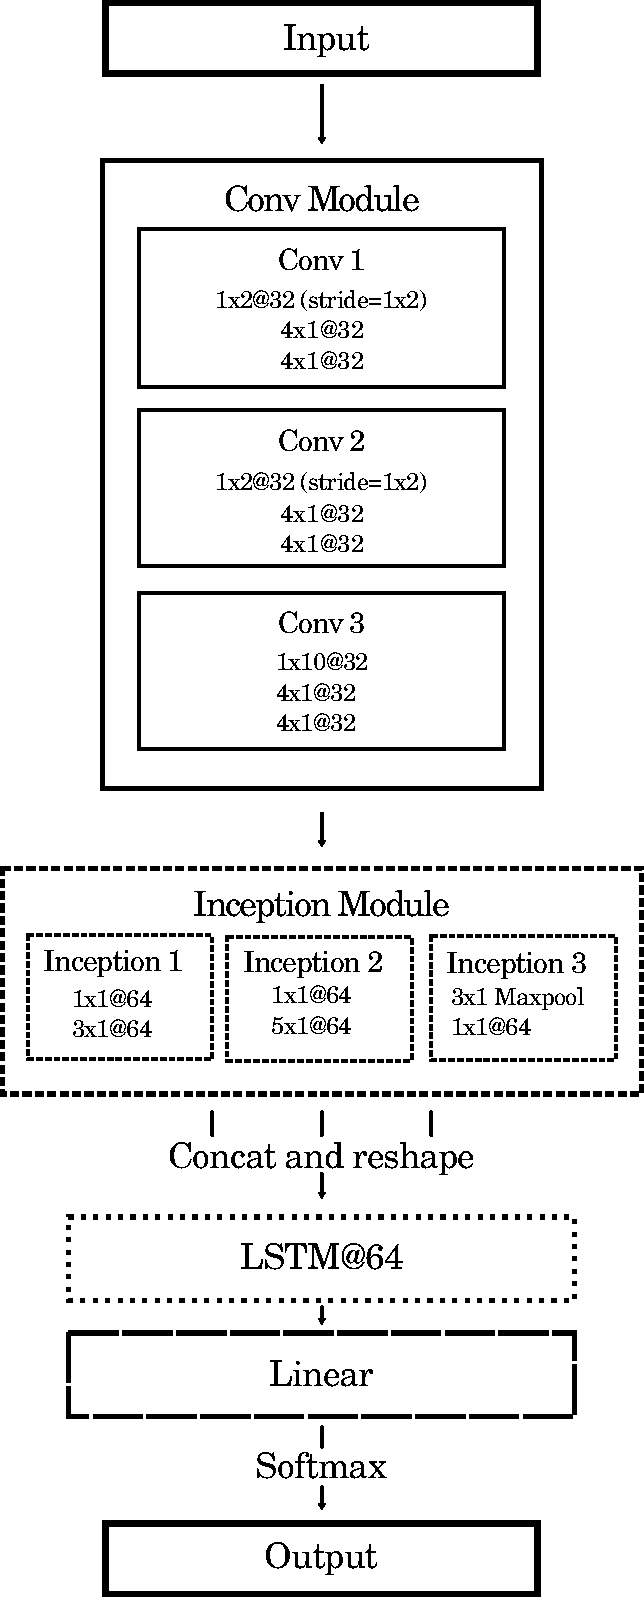
\includegraphics[width=0.50\textwidth]{./images/deepLOB_architecture_long.pdf}
    \caption{DeepLOB model architecture overview. Note: 1x2@32 denotes a convolutional layer with 32 filters and kernel size 1x2.}
    \label{fig:DeepLOB}
\end{figure}
\end{multicols}
\clearpage

\subsection{DeepOF}
Introduced in \cite{KOLM2023}, DeepOF is a modification of the DeepLOB architecture, using
OF features, rather than LOB features. \cite{KOLM2023} show that using orderflow
instead of the raw orderbook representation leads to better performance.
The DeepOF input is given by:

\begin{equation}
X_{t} := \begin{bmatrix}
e_{t-T, 1}^A & e_{t-T, 1}^B &   \cdots & e_{t-T, L}^A & e_{t-T, L}^B \\
e_{t-(T-1), 1}^A & e_{t-(T-1), 1}^B &   \cdots & e_{t-(T-1), L}^A & e_{t-(T-1), L}^B \\
\vdots & \vdots & \ddots & \vdots & \vdots \\
e_{t-1, 1}^A & e_{t-1, 1}^B &  \cdots & e_{t-1, L}^A & e_{t-1, L}^B \\
e_{t, 1}^A & e_{t, 1}^B &  \cdots & e_{t, L}^A & e_{t, L}^B \\
\end{bmatrix} \in \mathbb{R}^{T \times 2L}
\label{DeepLOB_input}
\end{equation}
where we have extended the tick level orderflow definition from (\ref{eBeA}) to any arbitrary orderbook level, $\ell$:
\begin{equation}
    \begin{aligned}
        e_{t, \ell}^B &:= I_{\{p_{t, \ell}^B \ge p_{t-1, \ell}^B\}} q_{t, \ell}^B - I_{\{p_{t, \ell}^B \le p_{t-1, \ell}^B\}} q_{t-1, \ell}^B \\
        e_{t, \ell}^A &:= I_{\{p_{t, \ell}^A \le p_{t-1, \ell}^A\}} q_{t, \ell}^A - I_{\{p_{t, \ell}^A \ge p_{t-1, \ell}^A\}} q_{t-1, \ell}^A
    \end{aligned}
\end{equation}
In terms of model architecture, the DeepOF model is the same as the DeepLOB model, except without
the first convolutional block, Conv 1. Recall that this block aggregates the price and volume information
from the LOB input, so by using OF input, we have essentially aggregated the price and volume information manually
using a predefined feature transform that has been shown to be predictive of mid-price movement. \cite{CONT2013}, \cite{KOLM2023}.

\section{Methodology}

\subsection{Sliding Window Setup}
We use a sliding window evaluation method, with train, validation and testing splits.
See Figure \ref{fig:slidingwindow} for a visual representation
of the splits.

\begin{figure}[htpb]
    \centering
    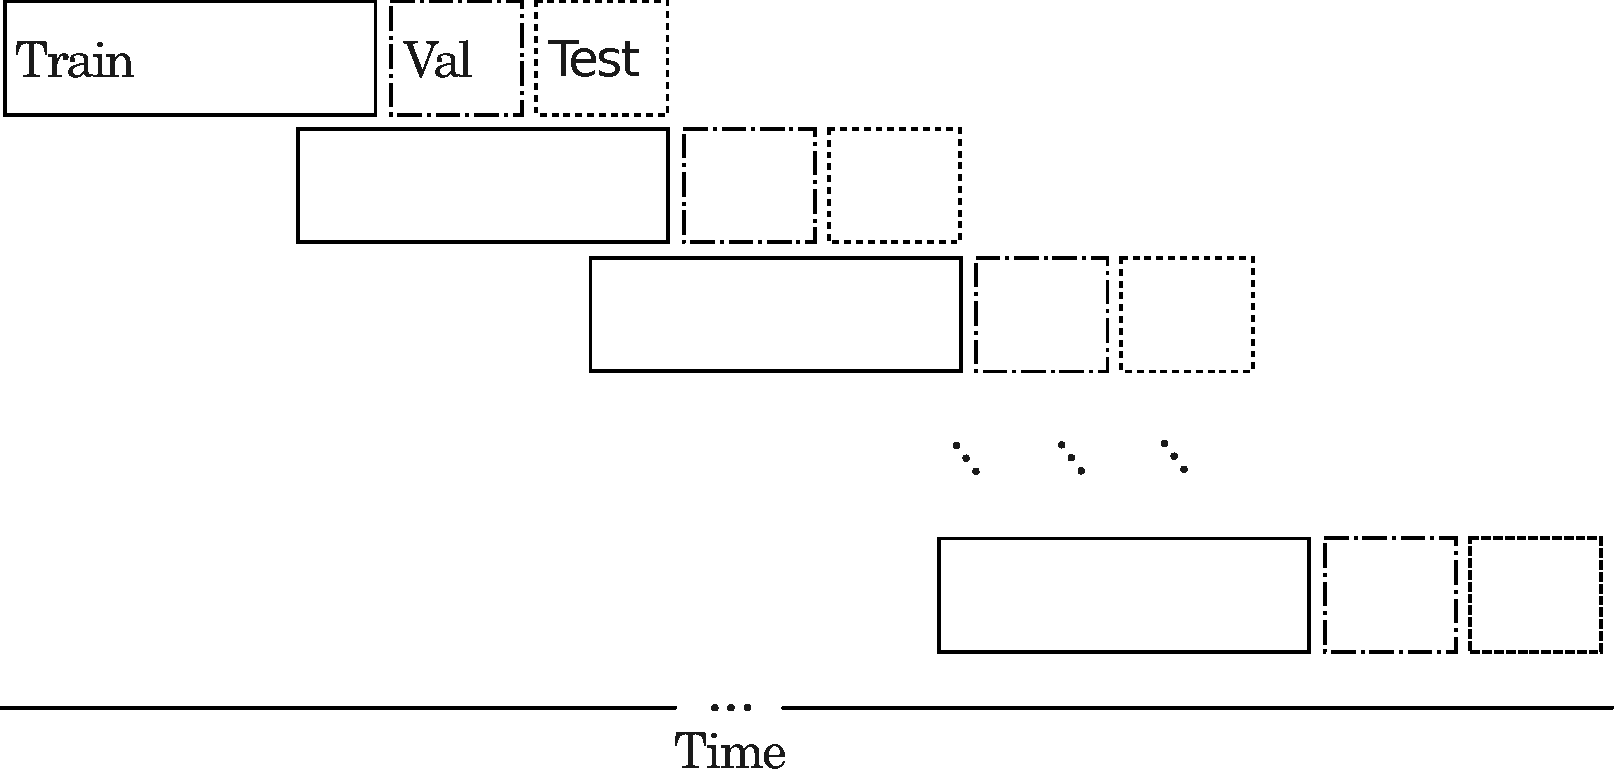
\includegraphics[width=1.0\textwidth]{./images/sliding_window.pdf}
    \caption{Sliding window visualization.}
    \label{fig:slidingwindow}
\end{figure}

So using this method we are able to validate and test on almost the entire dataset,
and only train on recent, relevant information. Note that we leave gaps between the train,
val and test blocks to avoid data leakage from features that look back in time.
We fix the length of the initial training window to 48 hours and the validation and testing windows to 24 hours each.

The general testing procedure will be to train on the training set, then fine-tune our hyperparameters using
the validation set, then once all of our hyperparameters have been chosen, 
we will test on the test set. Of course this means there will be a gap of 24 hours between our training
and testing data. We could alternatively merge the training and validation data once hyperparameter tuning is
complete and then re-train our models on the merged data before testing. However, leaving this gap
will provide an extra guarantee of robustness and provide a better picture of the out of sample
performance of our models.

\subsection{Data Normalization}
For several of our models, data normalization is important in order to ensure stable training
and convergence. \cite{LUCCHESE2024} and \cite{ZHANG2019} use five day rolling window normalization
whereas \cite{KOLM2023} use $z$-scores calculated using the training data.
We find the rolling window normalization method to give worse performance, since it transforms
our data in a non-linear way and so, for example, periods of no price change are
no longer flat. So following \cite{KOLM2023}, for each train-val-test window we calculate the 
sample mean and standard deviation of the training data, and use these to scale the training,
validation and testing data via $z$-scores.
% , i.e 
% \begin{equation}
%     \begin{aligned}
%         \hat{\mu}_{\text{train}} &:= \frac{1}{n_{\text{train}}} \sum_{i=1}^{n_{\text{train}}} X[i, :] \\
%         \hat{\sigma}_{\text{train}} &:= \frac{1}{n_{\text{train}}} \sum_{i=1}^{n_{\text{train}}} (X[i, :] - \hat{\mu}_{\text{train}})^2 \\
%         \tilde{X}_{\text{train}} &:= \frac{X_{\text{train}} - \hat{\mu}_{\text{train}}}{\hat{\sigma}_{\text{train}}} \\
%         \tilde{X}_{\text{val}} &:= \frac{X_{\text{val}} - \hat{\mu}_{\text{train}}}{\hat{\sigma}_{\text{train}}} \\
%         \tilde{X}_{\text{test}} &:= \frac{X_{\text{test}} - \hat{\mu}_{\text{train}}}{\hat{\sigma}_{\text{train}}}
%     \end{aligned}
% \end{equation}

\subsection{Choice of label discretization parameter}
Following \cite{LUCCHESE2024}, we set our discretization parameter, $\epsilon$, from (\ref{desc})
for each $k$ and train-val-test window, $w$, so that the classes are roughly balanced. i.e.
\begin{equation}
    \epsilon := \epsilon_{k, w} := \frac{|\hat{F}_{k, w}^{-1}(\frac{1}{3})| + \hat{F}_{k, w}^{-1}(\frac{2}{3})}{2}
\end{equation}
Where $\hat{F}_{k, w}$ is the empirical distribution of the training set $\ell(t)$, (\ref{smoothed_returns}), smoothed returns 
for prediction horizon $k$, and window $w$.


\subsection{Model Training}
Our DeepLOB and DeepOF models were trained with PyTorch, \cite{PYTORCH2017},
on an Nvidia RTX 3060 12GB with 64GB memory and a 14-core 20-thread Intel i5 13600K.
We use the ADAM optimizer, \cite{ADAM2017}, with learning rate set to $0.0001$.
For our loss function we use the Cross Entropy Loss, \cite{CROSSENTROPYLOSS}.
We trained our models until the validation loss plateaued and then used
the model from the epoch with highest validation loss.
% Our model 
% input is $(minibatch, C)$
% $$
% l_{n} = -w_{y_{n}} \log \frac{\exp(x_{n, y_{n}})}{\sum_{c=1}^C \exp(x_{n, c})softmax
% $$
% $$
% l(x, y) = \sum_{n=1}^N \frac{1}{\sum_{m=1}^N w_{y_{m}}} l_{n}
% $$
% ...
\clearpage

\section{Results}

\subsection{Classification Metrics}

Recall that this is a multi-class classification problem, with our three classes,
$-1$, for negative smoothed mid-price change, $0$ for insignificant smoothed mid-price change and $+1$ for positive mid-price change. 
This is an imbalanced problem, where we have up to $4 \times$ more $0$ labels for small $k$ compared with
$-1$ or $+1$ labels, since small time frames often mean no significant price change.
For this reason, accuracy is perhaps not the only metric we should care about.
In this case, \textit{precision}, \textit{recall} and \textit{F1} scores are often more insightful, \cite{HASTIE2001}.
Precision for class $ c $ is defined as:
\begin{equation}
\text{Precision}_c := \frac{\text{TP}_c}{\text{TP}_c + \text{FP}_c}
\end{equation}
where:
\begin{itemize}
    \item $ \text{TP}_c $ is the number of true positives for class $c$.
    \item $ \text{FP}_c $ is the number of false positives for class $c$.
\end{itemize}
So essentially, precision says: \textit{``out of all the times that we guessed class $c$, how many times were we correct?''}

Recall for class $c$ is defined as:
\begin{equation}
\text{Recall}_c := \frac{\text{TP}_c}{\text{TP}_c + \text{FN}_c}
\end{equation}
where:
\begin{itemize}
    \item $ \text{TP}_c $ is the number of true positives for class $c$.
    \item $ \text{FN}_c $ is the number of false negatives for class $c$.
\end{itemize}
So essentially, recall says: \textit{``out of all the times the true class was $c$, how many times did we predict it correctly?''}

F1-score for class $ c $ is the harmonic mean of precision and recall, defined as:
\begin{equation}
\text{F1-score}_c := 2 \cdot \frac{\text{Precision}_c \cdot \text{Recall}_c}{\text{Precision}_c + \text{Recall}_c}
\end{equation}

To get the overall performance across all classes, we can compute the macro-averaged precision, recall, and F1-score:
\begin{equation}
\text{Macro-Precision} := \frac{1}{3} \sum_{c \in \{-1,0,+1\}} \text{Precision}_c
\end{equation}

\begin{equation}
\text{Macro-Recall} := \frac{1}{3} \sum_{c \in \{-1,0,+1\}} \text{Recall}_c
\end{equation}

\begin{equation}
\text{Macro-F1-score} := \frac{1}{3} \sum_{c \in \{-1,0,+1\}} \text{F1-score}_c
\end{equation}

i.e. the unweighted mean. We can also define the weighted-average which weights each classes'
score according to their support. (Support for class $c$ is the number of instances of that class in the ground truth test labels).

\subsection{Model Results}
As previously stated, we train our models on the training windows, then validate
and tune our hyperparameters on the validation windows and then test on the test windows.
We present the results of the models on the test windows here.

We calculate the macro-averaged metrics on the test set for $k \in \{4, 10, 50, 200\}$ and present
the results in tables \ref{macro_table_1} - \ref{macro_table_4}. For brevity, we only present the results for BTCUSDT here. We will delve deeper
into the comparative performance of each model for different trading pairs later on. See appendix for un-averaged model results for all trading pairs.


\begin{table}[H]
\resizebox{0.99\textwidth}{!}{
\begin{tabular}{llllll}
\toprule
accuracy & precision & recall & f1-score & support & model \\
\midrule
\textbf{0.87}(0.03) & \textbf{0.91}(0.03) & \textbf{0.74}(0.01) & \textbf{0.80}(0.01) & 647295(30003) & \textbf{xgbOF} \\
0.79(0.04) & 0.75(0.05) & 0.68(0.02) & 0.70(0.01) & 647295(30003) & xgbLOB \\
0.84(0.04) & 0.87(0.02) & 0.70(0.01) & 0.76(0.01) & 647289(30003) & lrOF \\
0.69(0.07) & 0.66(0.08) & 0.60(0.07) & 0.59(0.06) & 647289(30003) & lrLOB \\
0.86(0.03) & 0.88(0.03) & \textbf{0.74}(0.01) & 0.79(0.0) & 647199(30003) & deepOF \\
0.75(0.2) & 0.73(0.22) & 0.70(0.04) & 0.69(0.17) & 647199(30003) & deepLOB \\
\bottomrule
\end{tabular}
}
\caption{Mean macro averaged BTCUSDT test set classification results across windows for $\bm{k=4}$. (Standard deviations are given in parenthesis).}
\label{macro_table_1}
\end{table}

\begin{table}[H]
\resizebox{0.99\textwidth}{!}{
\begin{tabular}{llllll}
\toprule
accuracy & precision & recall & f1-score & support & model \\
\midrule
\textbf{0.80}(0.03) & \textbf{0.84}(0.04) & 0.75(0.01) & \textbf{0.78}(0.02) & 647289(30003) & \textbf{xgbOF} \\
0.72(0.02) & 0.71(0.02) & 0.71(0.01) & 0.71(0.01) & 647289(30003) & xgbLOB \\
0.76(0.04) & 0.81(0.03) & 0.72(0.01) & 0.74(0.02) & 647289(30003) & lrOF \\
0.58(0.07) & 0.62(0.05) & 0.62(0.04) & 0.57(0.08) & 647289(30003) & lrLOB \\
0.79(0.03) & 0.81(0.02) & \textbf{0.76}(0.01) & 0.77(0.01) & 647199(30003) & deepOF \\
0.74(0.06) & 0.76(0.04) & 0.71(0.05) & 0.72(0.06) & 647199(30003) & deepLOB \\
\bottomrule
\end{tabular}
}
\caption{Mean macro averaged BTCUSDT test set classification results across windows for $\bm{k=10}$.}
\label{macro_table_2}
\end{table}

\begin{table}[H]
\resizebox{0.99\textwidth}{!}{
    \begin{tabular}{llllll}
    \toprule
    accuracy & precision & recall & f1-score & support & model \\
    \midrule
    0.64(0.04) & \textbf{0.65}(0.03) & 0.62(0.01) & 0.63(0.02) & 647279(30003) & xgbOF \\
    0.56(0.04) & 0.57(0.03) & 0.58(0.04) & 0.53(0.06) & 647279(30003) & xgbLOB \\
    0.57(0.05) & 0.62(0.03) & 0.55(0.0) & 0.55(0.02) & 647289(30003) & lrOF \\
    0.51(0.06) & 0.52(0.03) & 0.54(0.03) & 0.46(0.06) & 647289(30003) & lrLOB \\
    \textbf{0.66}(0.03) & \textbf{0.65}(0.02) & \textbf{0.65}(0.02) & \textbf{0.65}(0.02) & 647199(30003) & \textbf{deepOF} \\
    0.57(0.07) & 0.58(0.04) & 0.57(0.07) & 0.55(0.09) & 647199(30003) & deepLOB \\
    \bottomrule
    \end{tabular}
}
\caption{Mean macro averaged BTCUSDT test set classification results across windows for $\bm{k=50}$.}
\label{macro_table_3}
\end{table}

\begin{table}[H]
\resizebox{0.99\textwidth}{!}{
    \begin{tabular}{llllll}
    \toprule
    accuracy & precision & recall & f1-score & support & model \\
    \midrule
    0.52(0.04) & 0.53(0.03) & 0.50(0.01) & 0.51(0.01) & 647279(30003) & xgbOF \\
    0.46(0.04) & 0.45(0.02) & 0.48(0.02) & 0.40(0.04) & 647279(30003) & xgbLOB \\
    0.48(0.05) & 0.50(0.02) & 0.46(0.01) & 0.45(0.01) & 647289(30003) & lrOF \\
    0.44(0.05) & 0.45(0.04) & 0.47(0.03) & 0.39(0.04) & 647289(30003) & lrLOB \\
    \textbf{0.56}(0.03) & \textbf{0.56}(0.02) & \textbf{0.55}(0.02) & \textbf{0.55}(0.02) & 647199(30003) & \textbf{deepOF} \\
    0.49(0.05) & 0.48(0.04) & 0.49(0.06) & 0.47(0.05) & 647199(30003) & deepLOB \\
    \bottomrule
    \end{tabular}
}
\caption{Mean macro averaged BTCUSDT test set classification results across windows for $\bm{k=200}$.}
\label{macro_table_4}
\end{table}

Overall we observe very decent performance with clear predictability. We see that for $k=4$ and $k=10$ 
xgbOF is the clear winner. We then see that deepOF takes over for $k=50$ and  $k=200$.
To give a clearer picture of comparative performance across windows, we plot the macro averaged
precision, recall and F1 for each trading pair, for each window and for each $k$ in Figures \ref{macro_plots_1} - \ref{macro_plots_4}.


We see that for $k=4$ and $k=10$, generally, xgbOF has the best precision and deepLOB has the best recall, with very similar
F1 scores. We also observe that, in general the models perform similarly for different trading pairs, with model rankings generally preserved,
although we do see a slightly decreased performance for trading pairs with lower trade volume. It seems that the general performance of our models
is an increasing function of trading pair liquidity when measured using macro F1.
This is an interesting result, and suggests that perhaps higher volume trading pairs are more predictable.

As we increase $k$ to $50$ and then $200$, we see that the deepOF model starts pulling away from the other models for all metrics.
This is perhaps due to the fact that deepOF has a much larger, $T=100$, lookback, whereas (due to memory constraints) our xgbOF model
has lookback $T = \min(k, 20) = 20$ for $k= 50, 100$.
We see that xgbOF and deepOF give the most stable results across windows in terms of variation. We see lrLOB has high variation
and performs poorly. Interestingly lrOF performs very well, often beating out the much larger deepLOB and xgbLOB models.
It is clear that the OF representation is far superior, since all OF based models generally exhibit superior performance
(when not constrained by lookback).

Of course, whilst macro-averaging gives a good overall idea of comparative performance, it averages performance across classes,
so therefore we don't yet have a clear picture of how our models perform comparatively for each class.
In Figures \ref{BTCUSDT_cm} - \ref{SOLUSDT_cm} we present confusion matrices, with counts summed across windows.

Again we see that for smaller $k$ values, this is a very imbalanced classification problem, with the majority
of the labels being class $0$, i.e. stationary mid-price change. We see that as we increase $k$ the distribution
of labels spreads out more equally across classes. We also observe that, all of our confusion matrices have most weight
along their diagonals, which is good news and means our models all perform better than randomly guessing.
We see that the distributions are symmetric for the $+1$ and $-1$ classes so henceforth, in our analysis
we will group these classes together and refer to them as the non-zero classes.

Recall that precision is defined as the number of correctly predicted labels for a class divided by the number of predicted labels for that
class, and recall is the number of correctly predicted labels for a class divided by the total number of labels for that class.
Using a poker analogy, precision tells us, out of all the times that we played a hand, what proportion of times did we win. Recall
tells us, out of all the times that we had a winning hand, how many times did we play and win.
So for a trading scenario, what we really care about is precision of the $+1$ and $-1$ classes, since for most applications, it would
be much more harmful to play and lose, rather than not play and miss a winning hand.
We see that the precision of the non-zero classes is much higher than the precision of the zero class, whereas the recall of the
non-zero classes is much lower than the recall of the zero class. This is due to the imbalanced nature of our labels, and we
see that, as we increase $k$, the precision and recall get closer. The precision of the non-zero classes is around 90\% for our best models for
small $k$, which is a great result for the reasons mentioned above.

We see that, as we move across trading pairs, we start seeing less weight on the zero labels and more predictions
for the non-zero classes. This is perhaps due to the fact that, for our test data, MATICUSDT and SOLUSDT have more balanced support, compared with BTCUSDT and ETHUSDT. i.e. the distribution of the true labels is less imbalanced for MATICUSDT and SOLUSDT.
This is perhaps due to MATICUSDT and SOLUSDT having higher volatility over our testing windows, so fewer non-zero price changes.

\begin{figure}[htpb!]
    \centering
    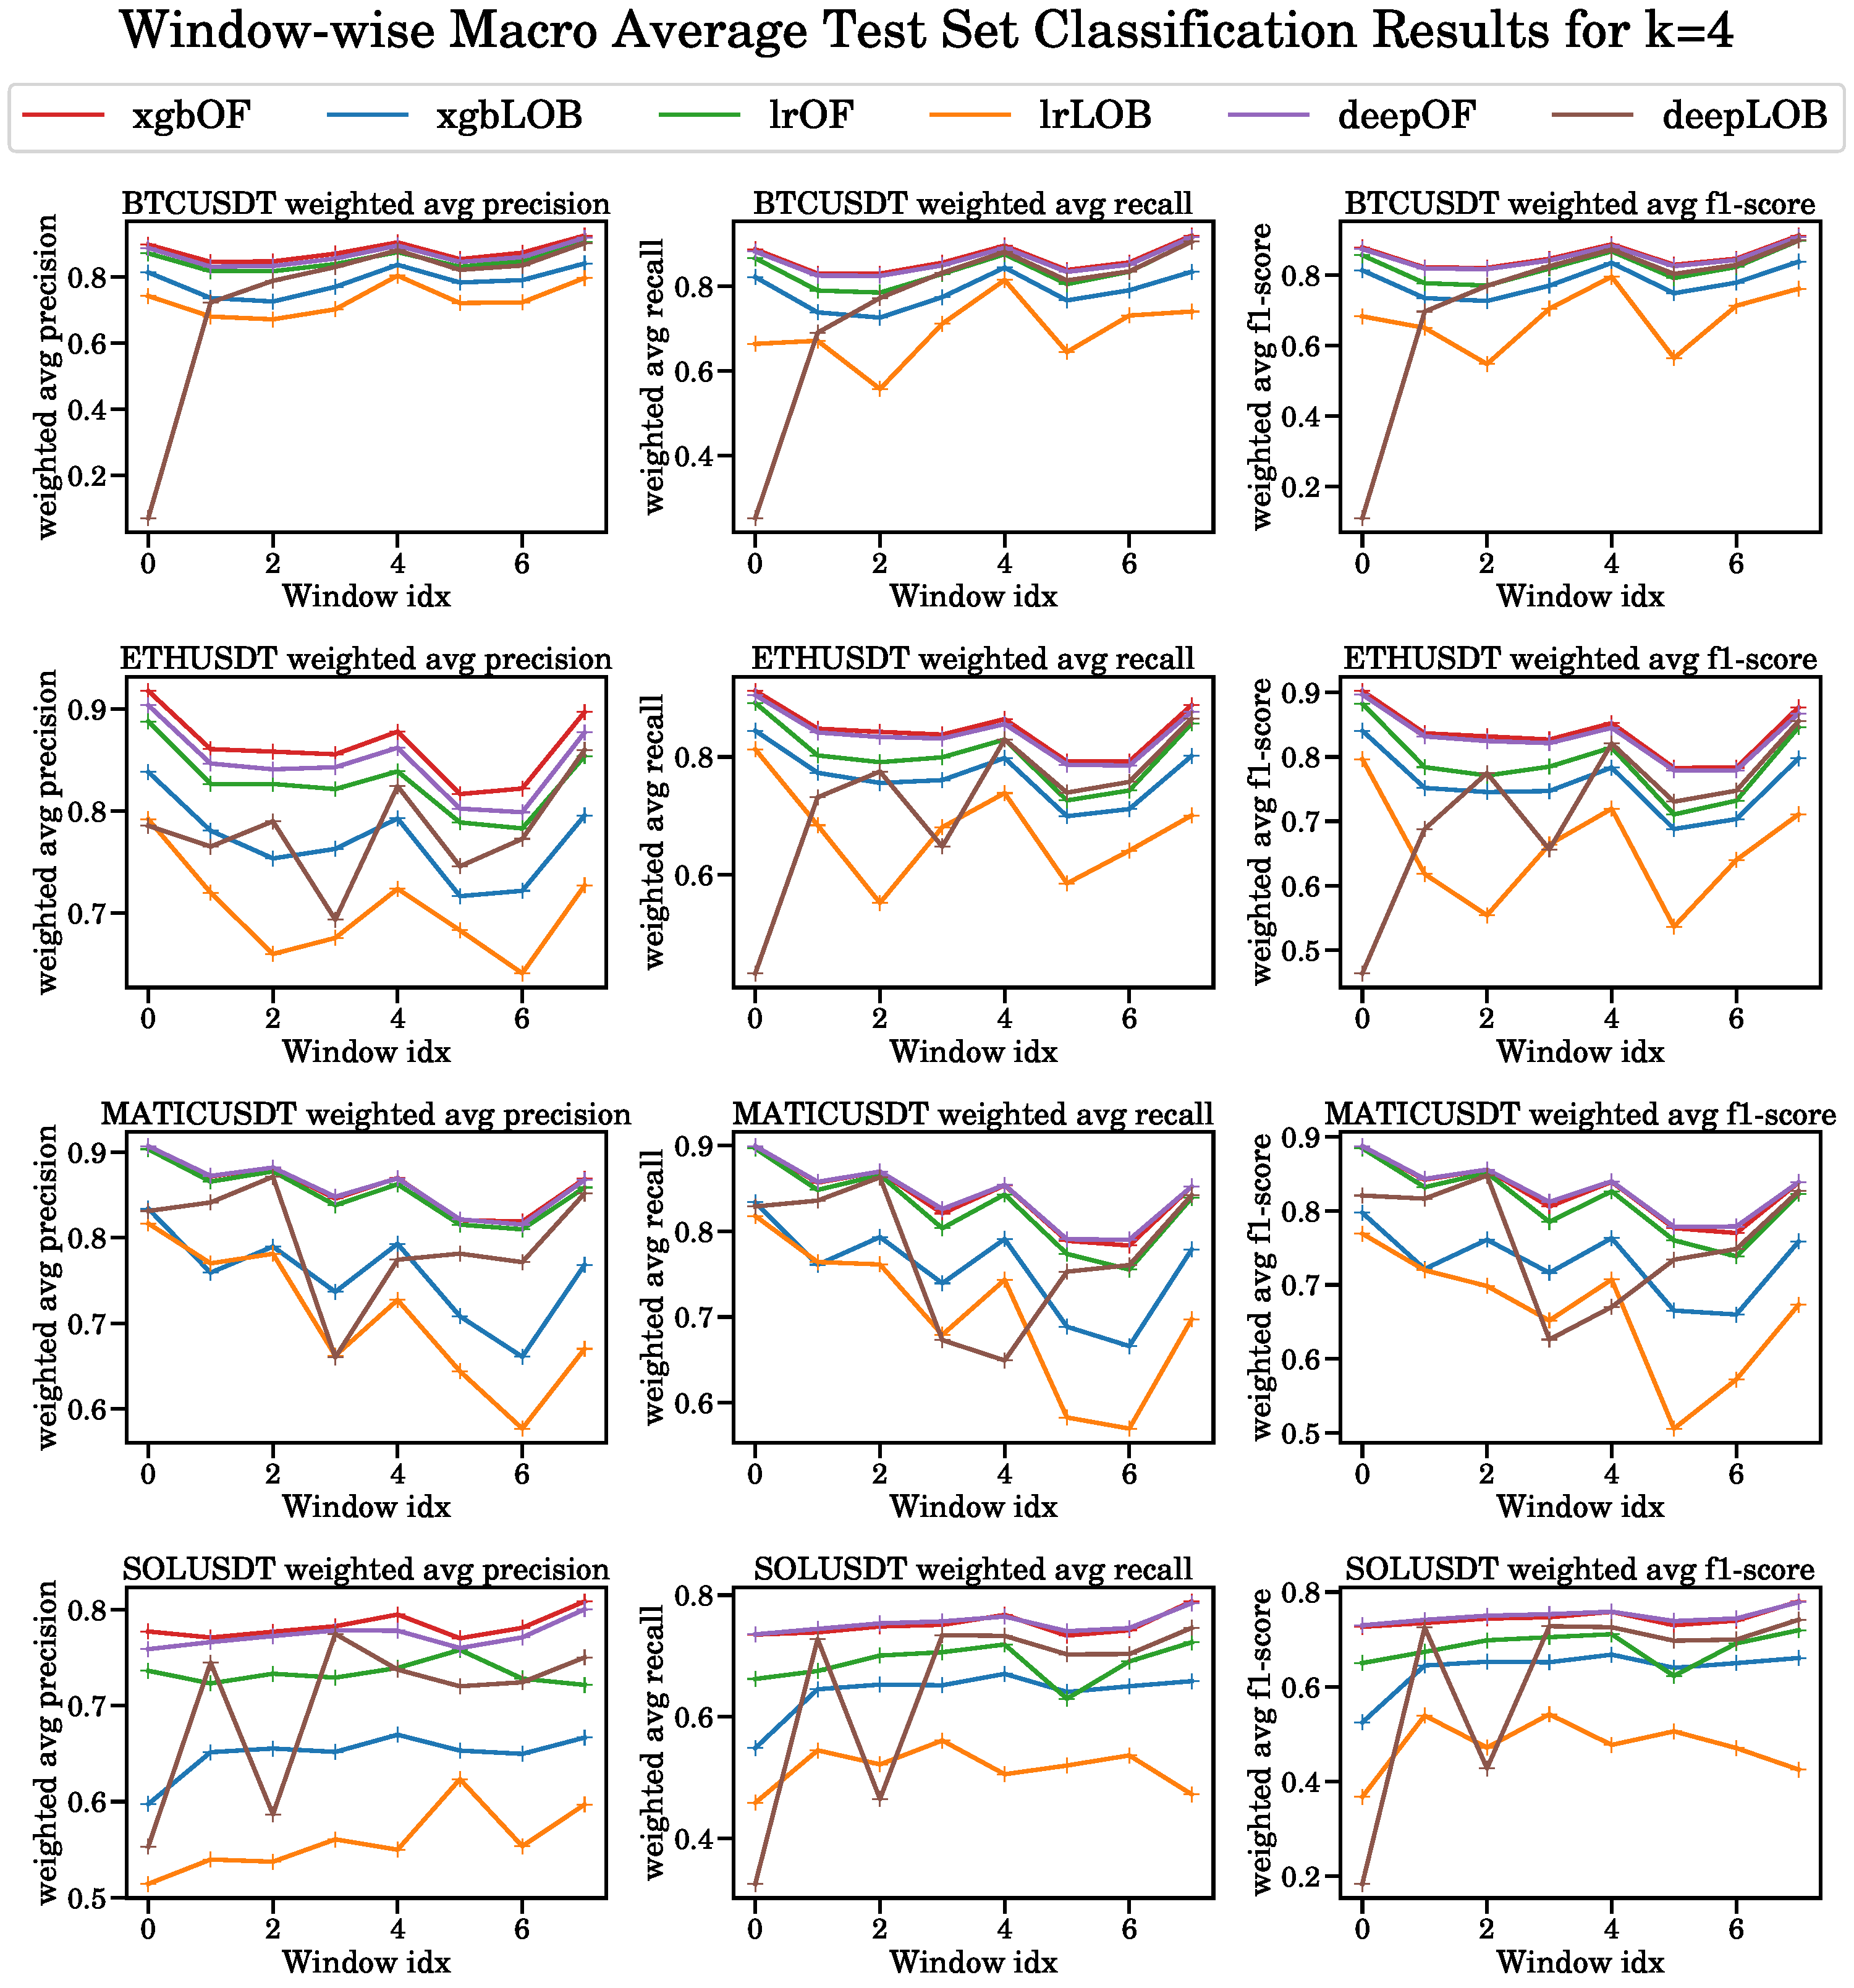
\includegraphics[width=0.93\textwidth]{./images/macro_results_k=4.pdf}
    \caption{Comparing the macro averaged precision, recall and F1 score on the unseen test set for each window, for each trading pair, for $k=4$.}
    \label{macro_plots_1}
\end{figure}

\begin{figure}[htpb!]
    \centering
    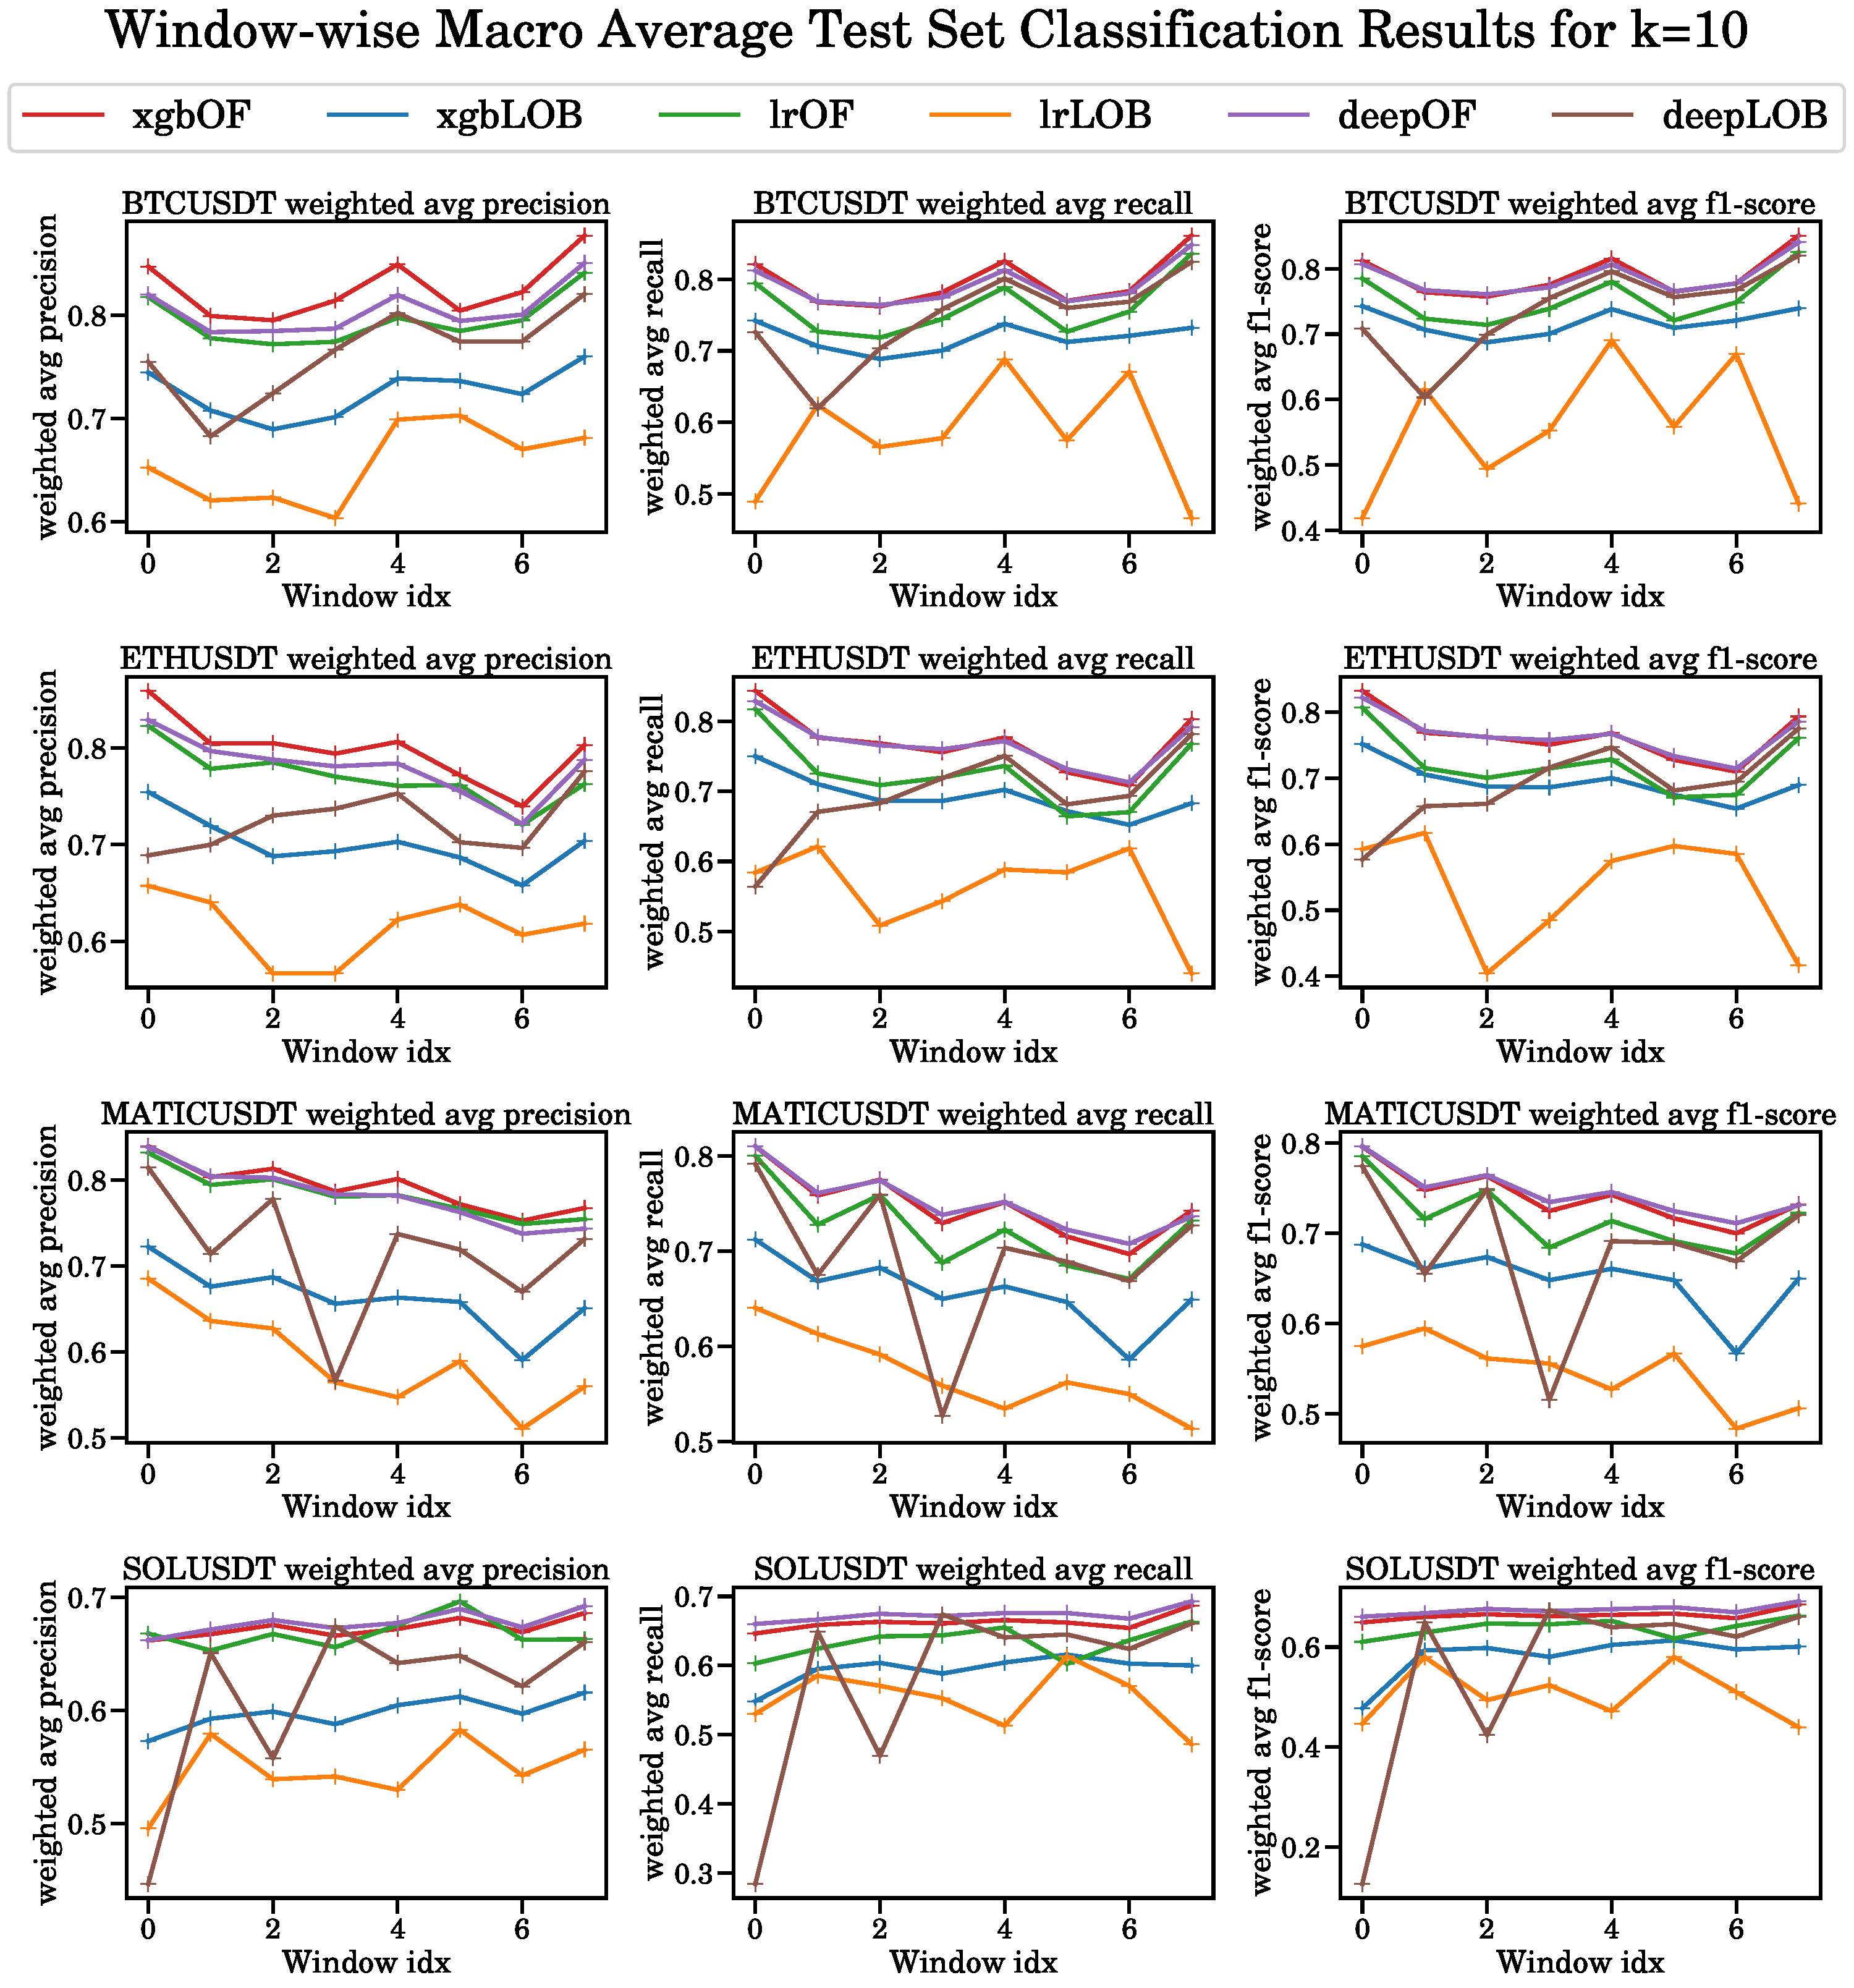
\includegraphics[width=1.0\textwidth]{./images/macro_results_k=10.pdf}
    \caption{Comparing the macro averaged precision, recall and F1 score on the unseen test set for each window, for each trading pair, for $k=10$.}
    \label{macro_plots_2}
\end{figure}

\begin{figure}[htpb!]
    \centering
    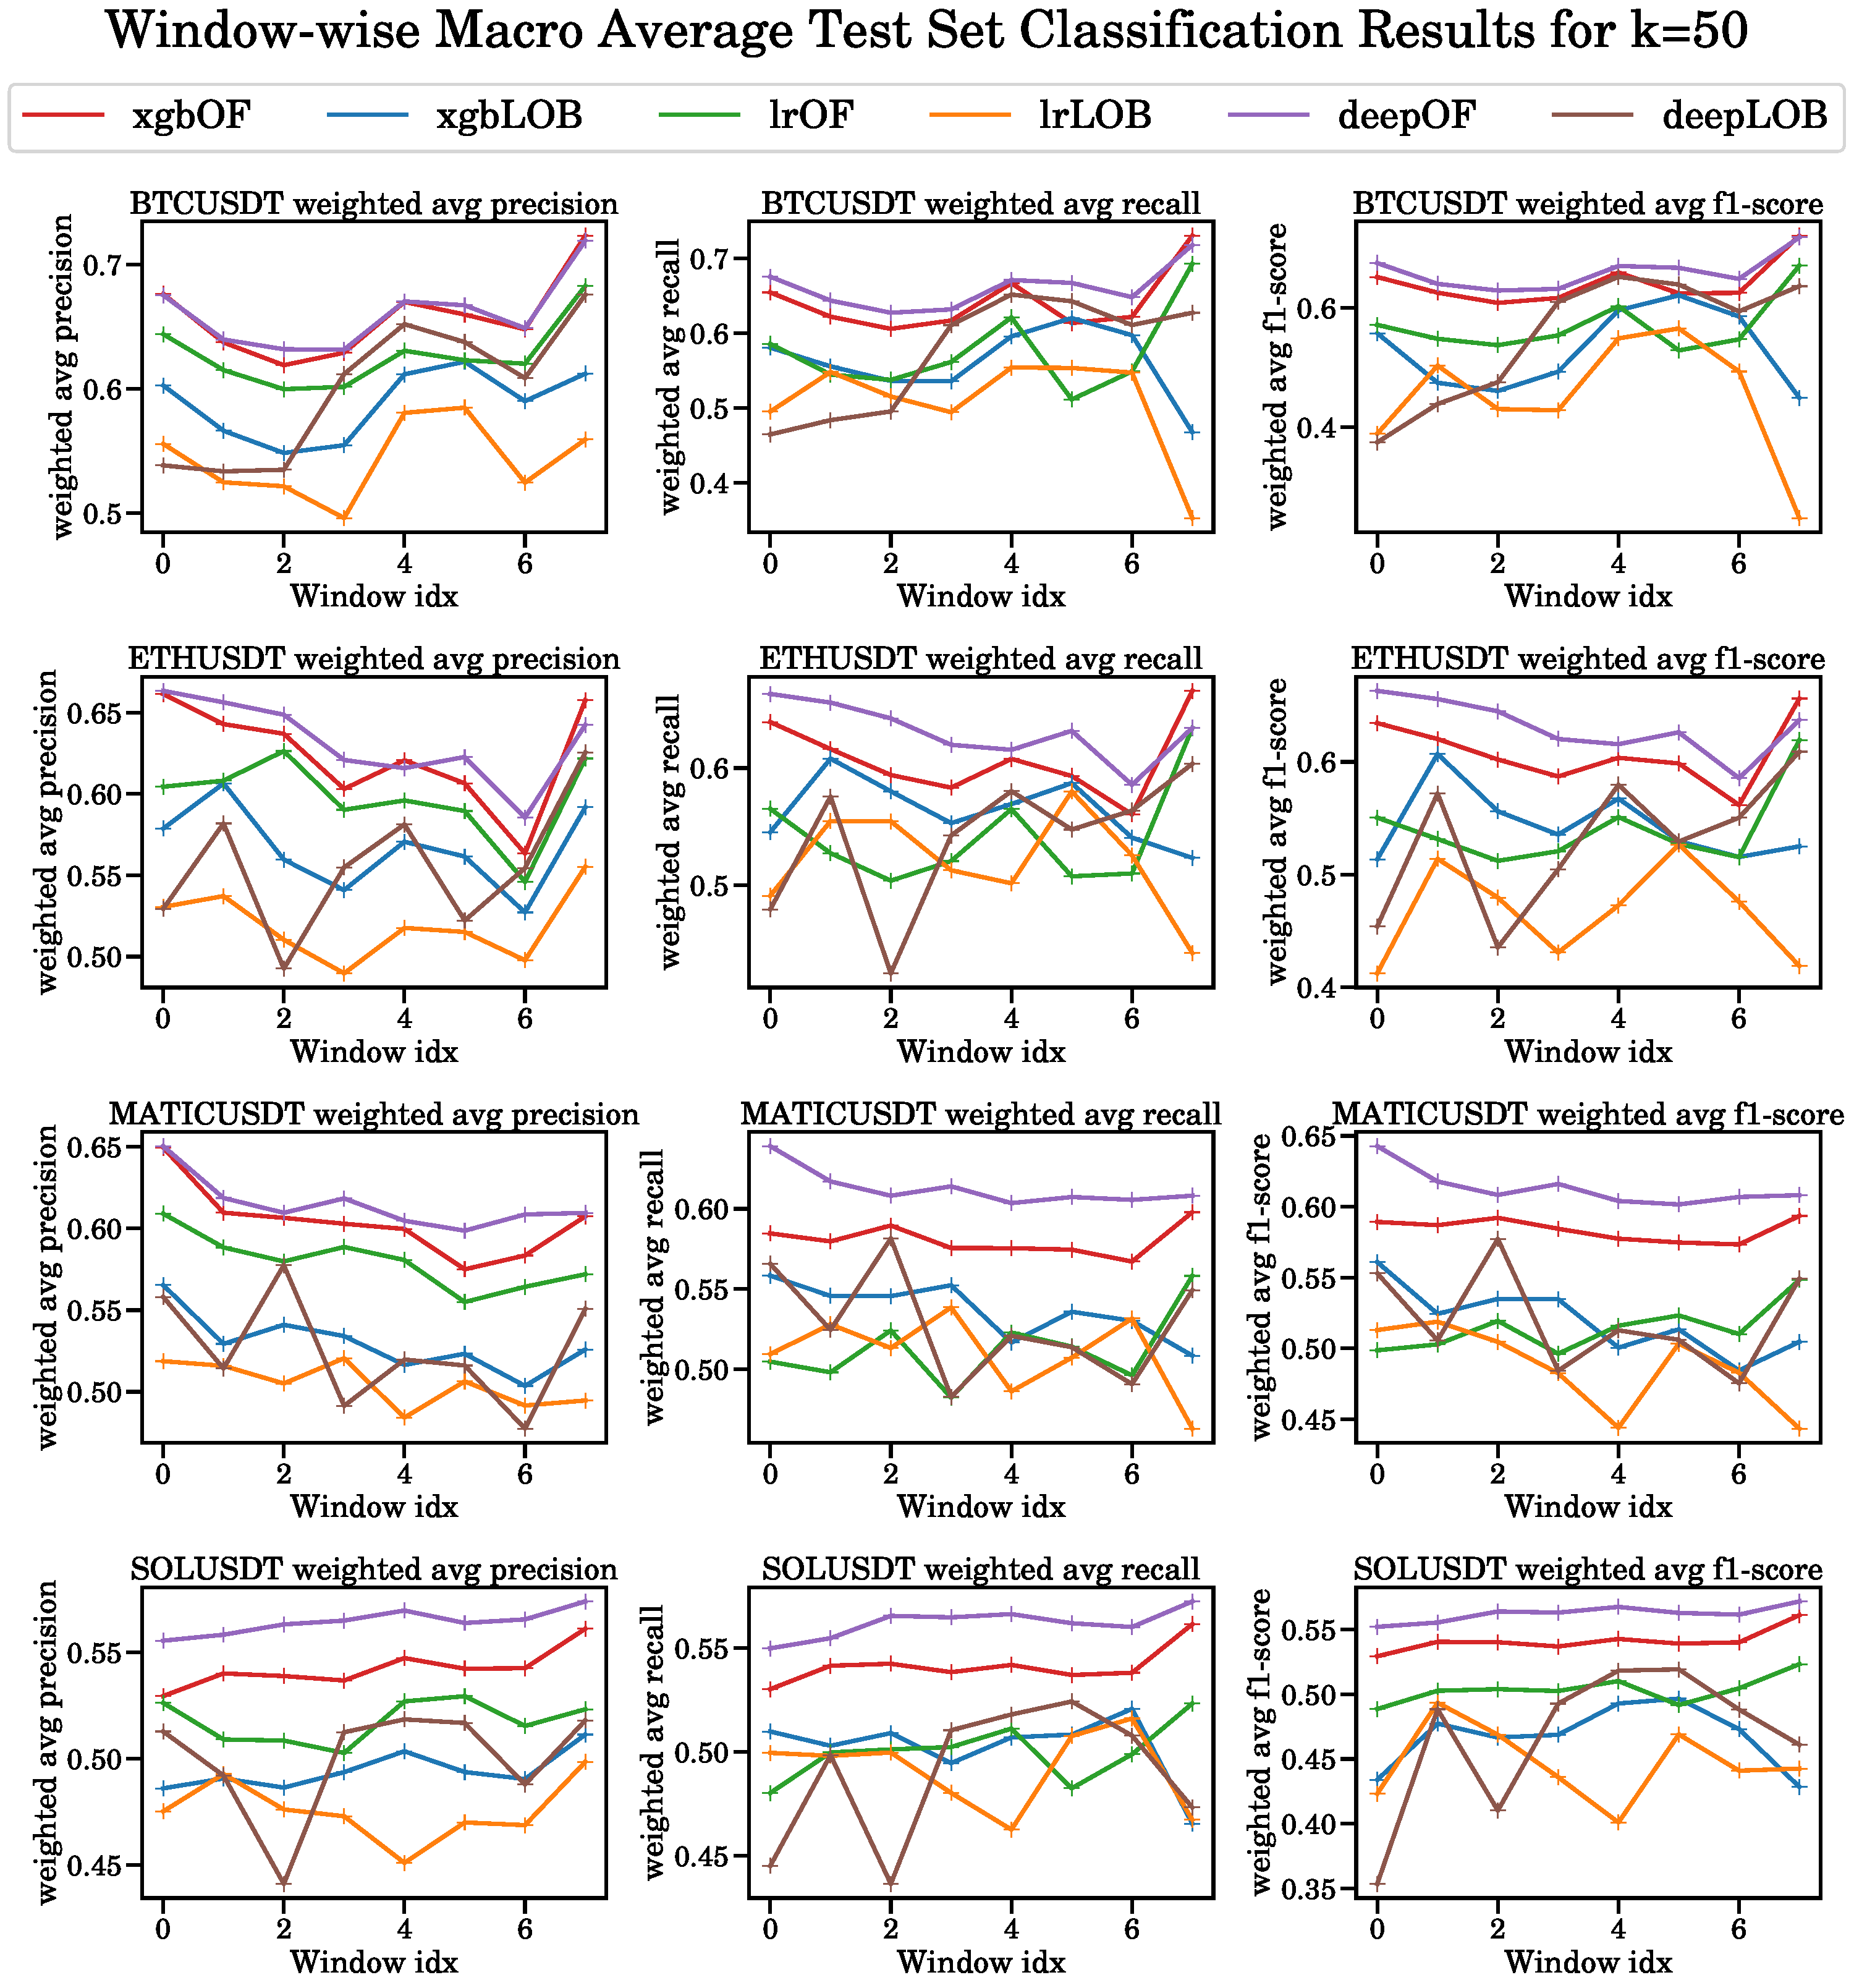
\includegraphics[width=1.0\textwidth]{./images/macro_results_k=50.pdf}
    \caption{Comparing the macro averaged precision, recall and F1 score on the unseen test set for each window, for each trading pair, for $k=50$.}
    \label{macro_plots_3}
\end{figure}

\begin{figure}[htpb!]
    \centering
    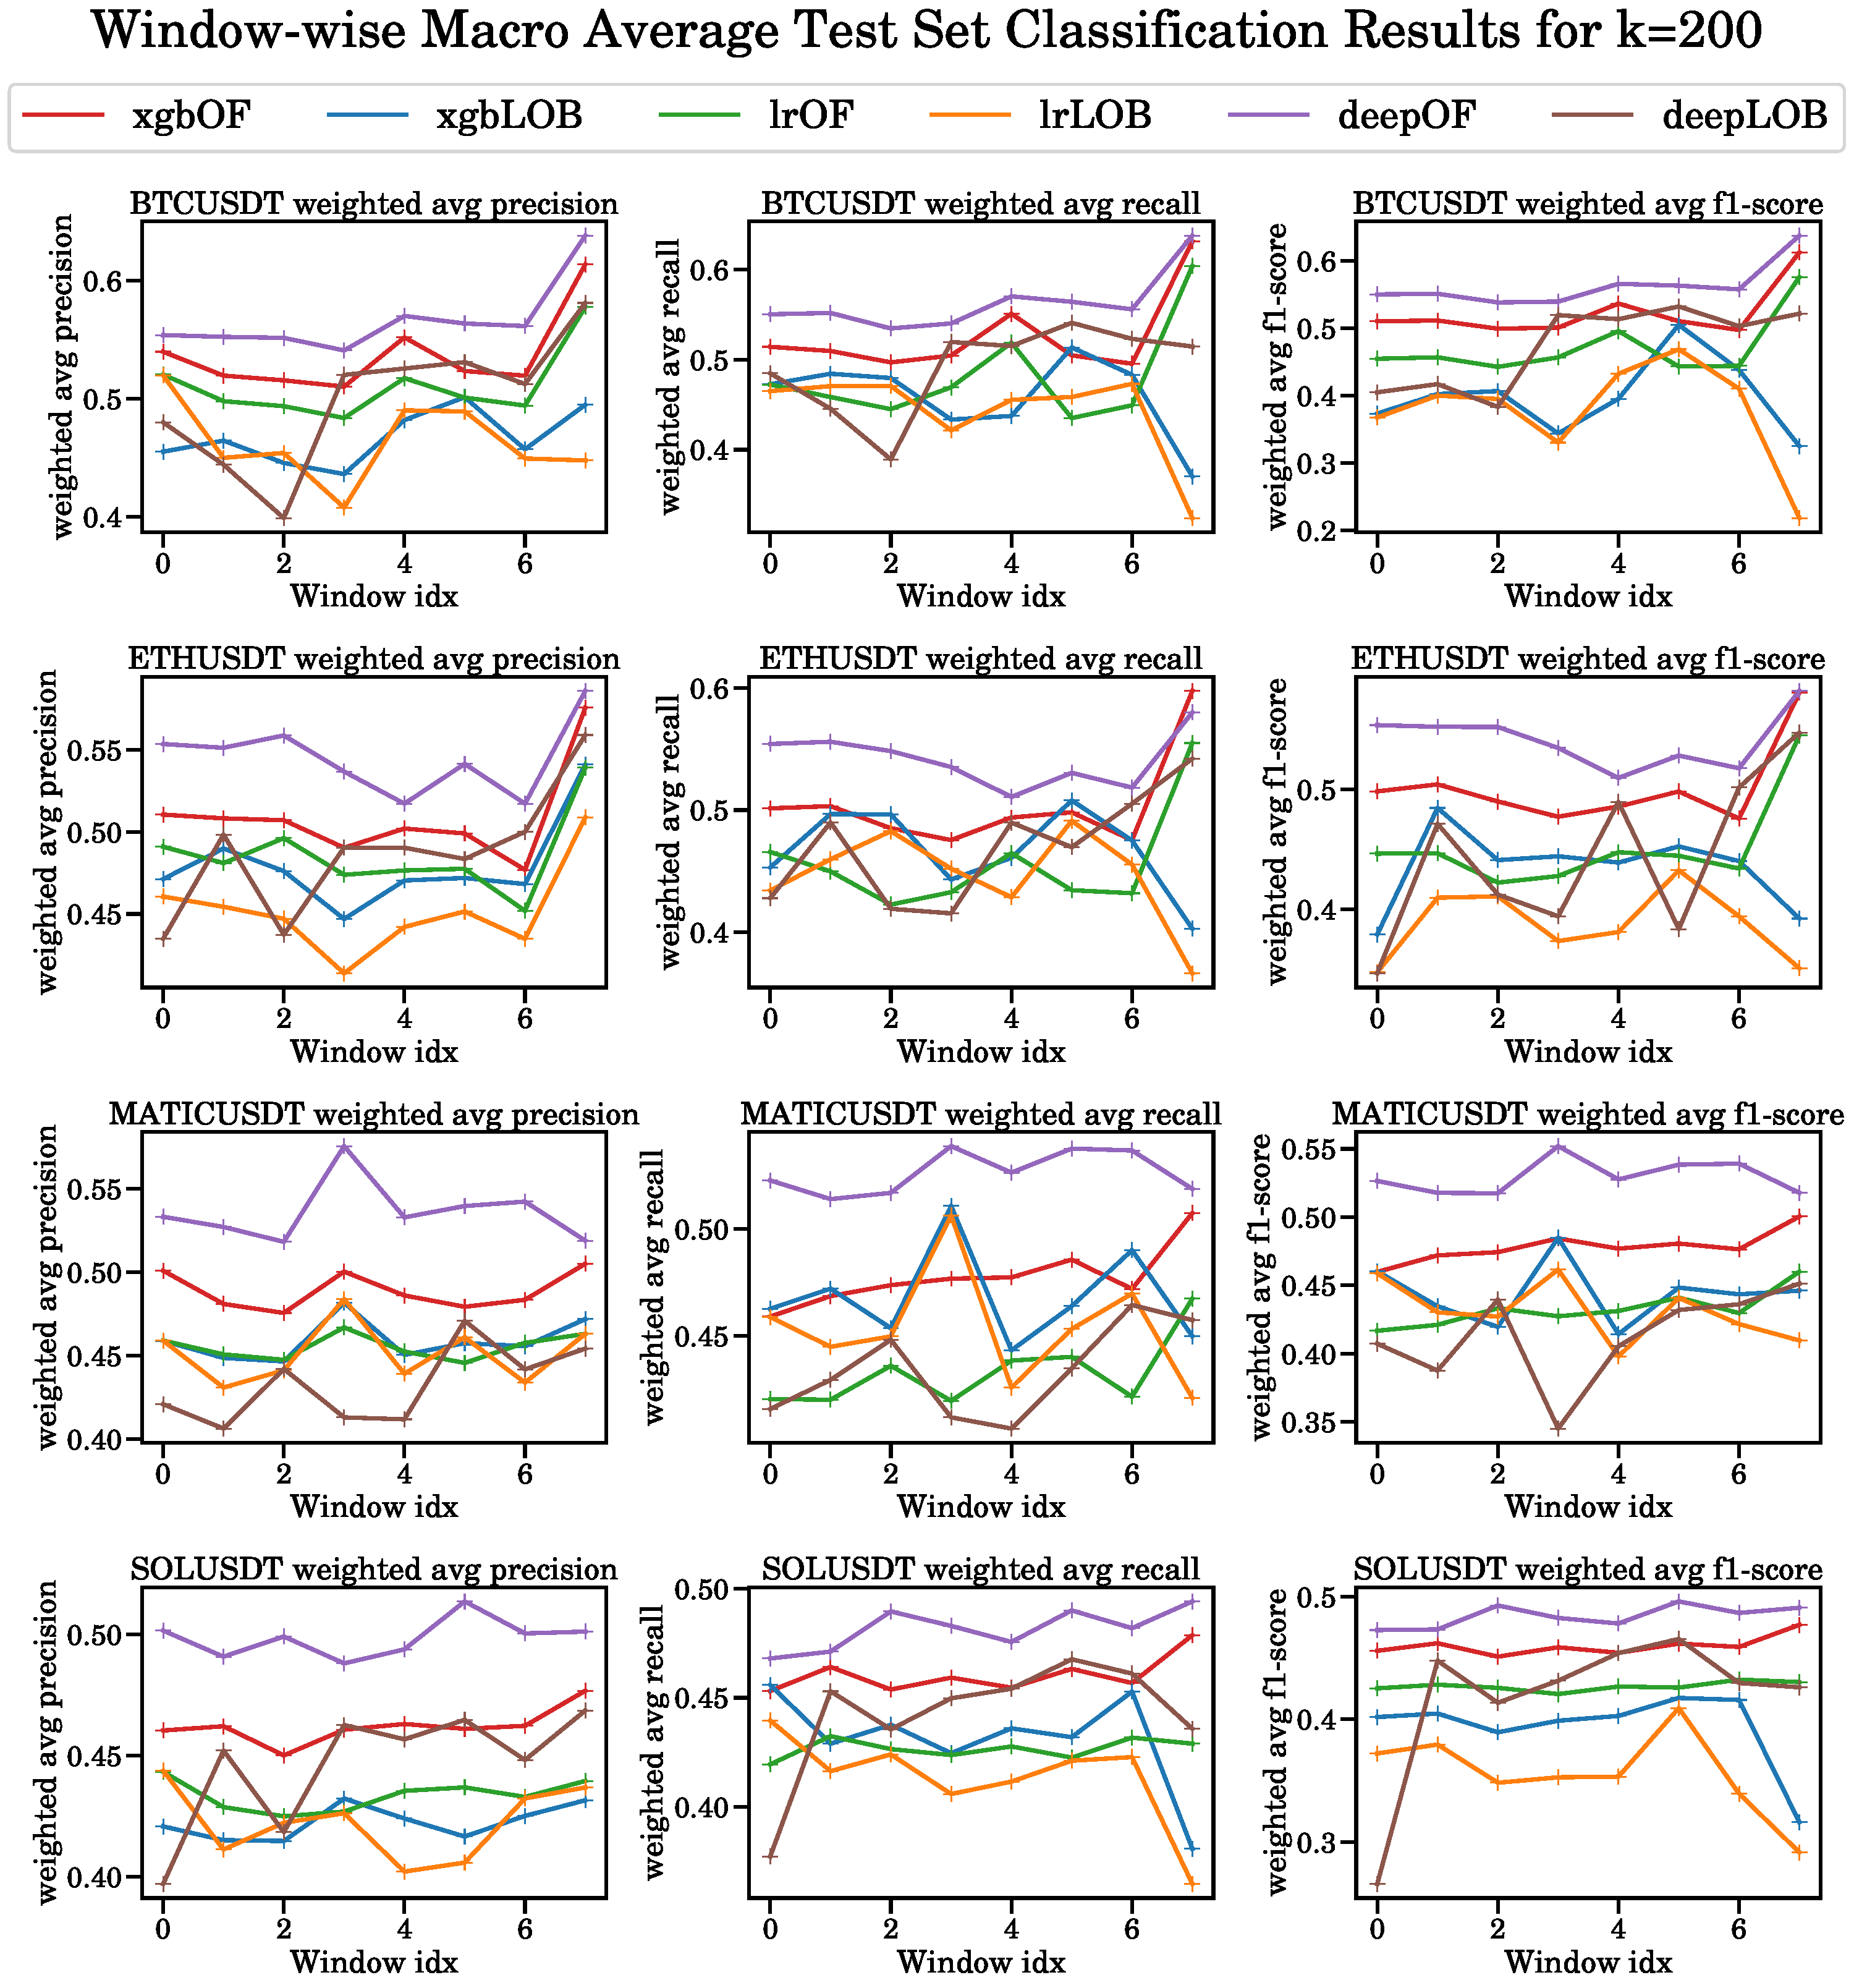
\includegraphics[width=1.0\textwidth]{./images/macro_results_k=200.pdf}
    \caption{Comparing the macro averaged precision, recall and F1 score on the unseen test set for each window, for each trading pair, for $k=200$.}
    \label{macro_plots_4}
\end{figure}

\begin{figure}[htpb!]
    \centering
    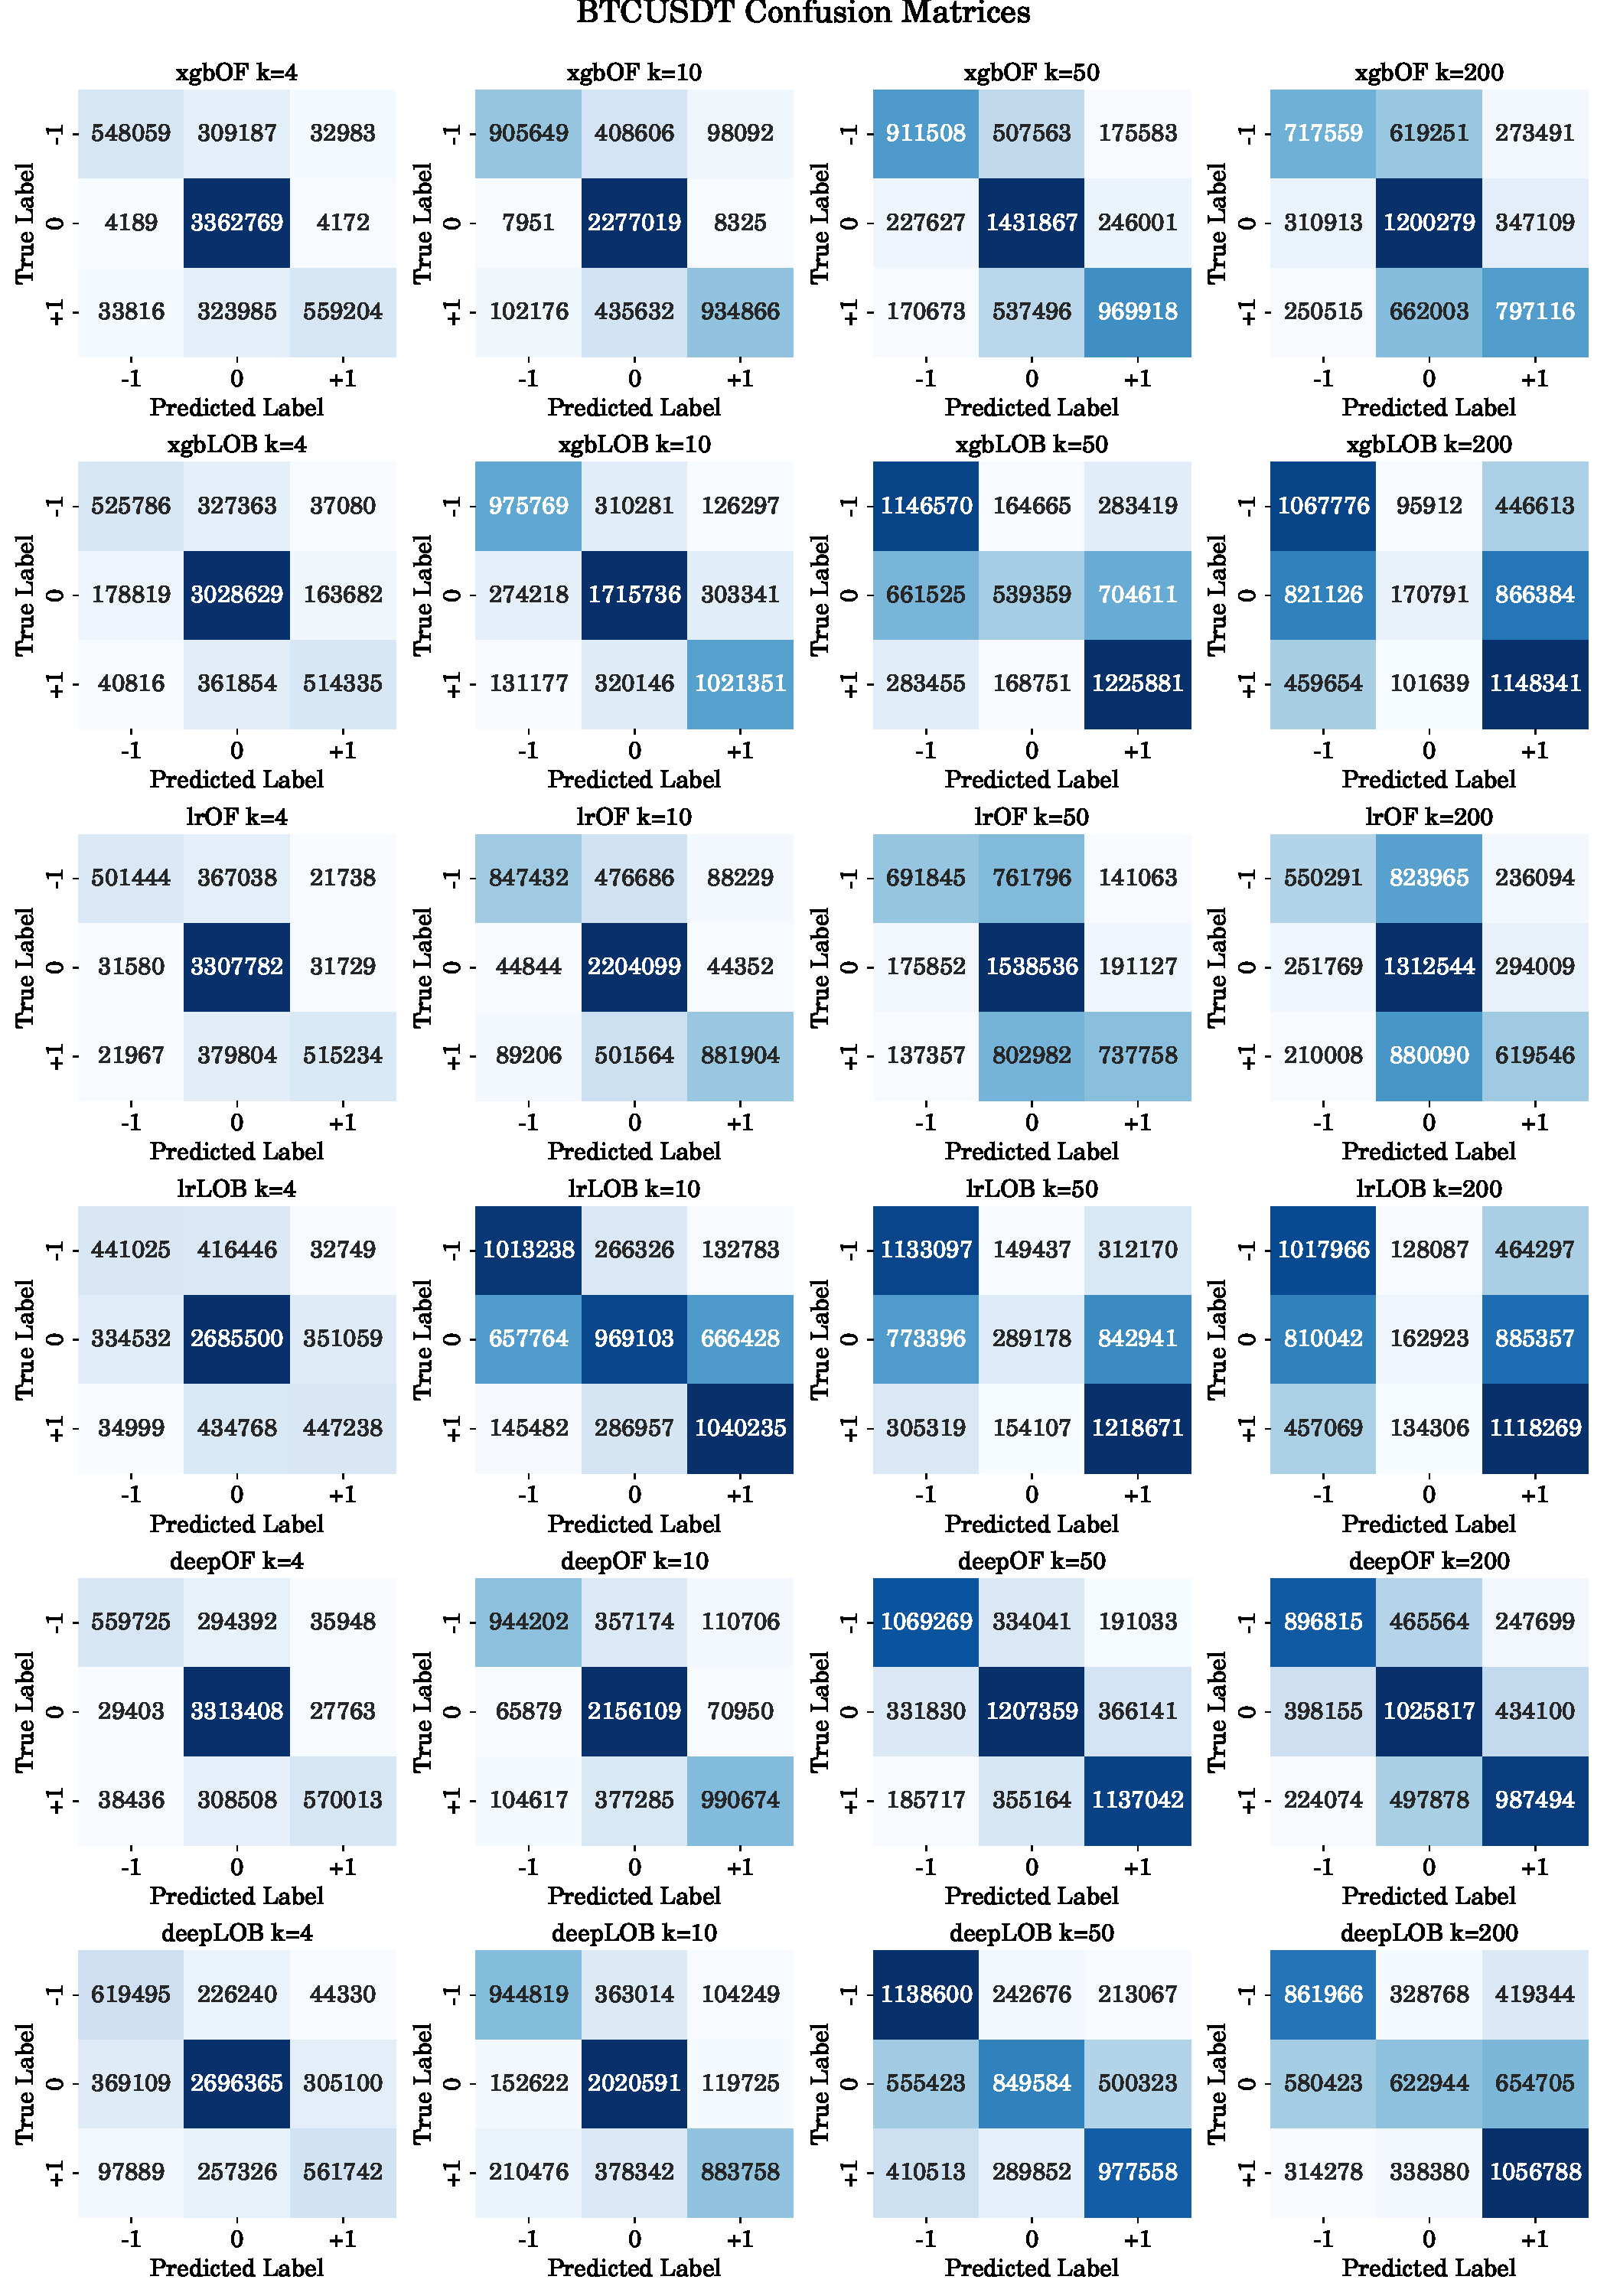
\includegraphics[width=1.0\textwidth]{./images/BTCUSDT_confusion_matrices.pdf}
    \caption{BTCUSDT confusion matrices. Note that counts are summed across windows.}
    \label{BTCUSDT_cm}
\end{figure}

\begin{figure}[htpb!]
    \centering
    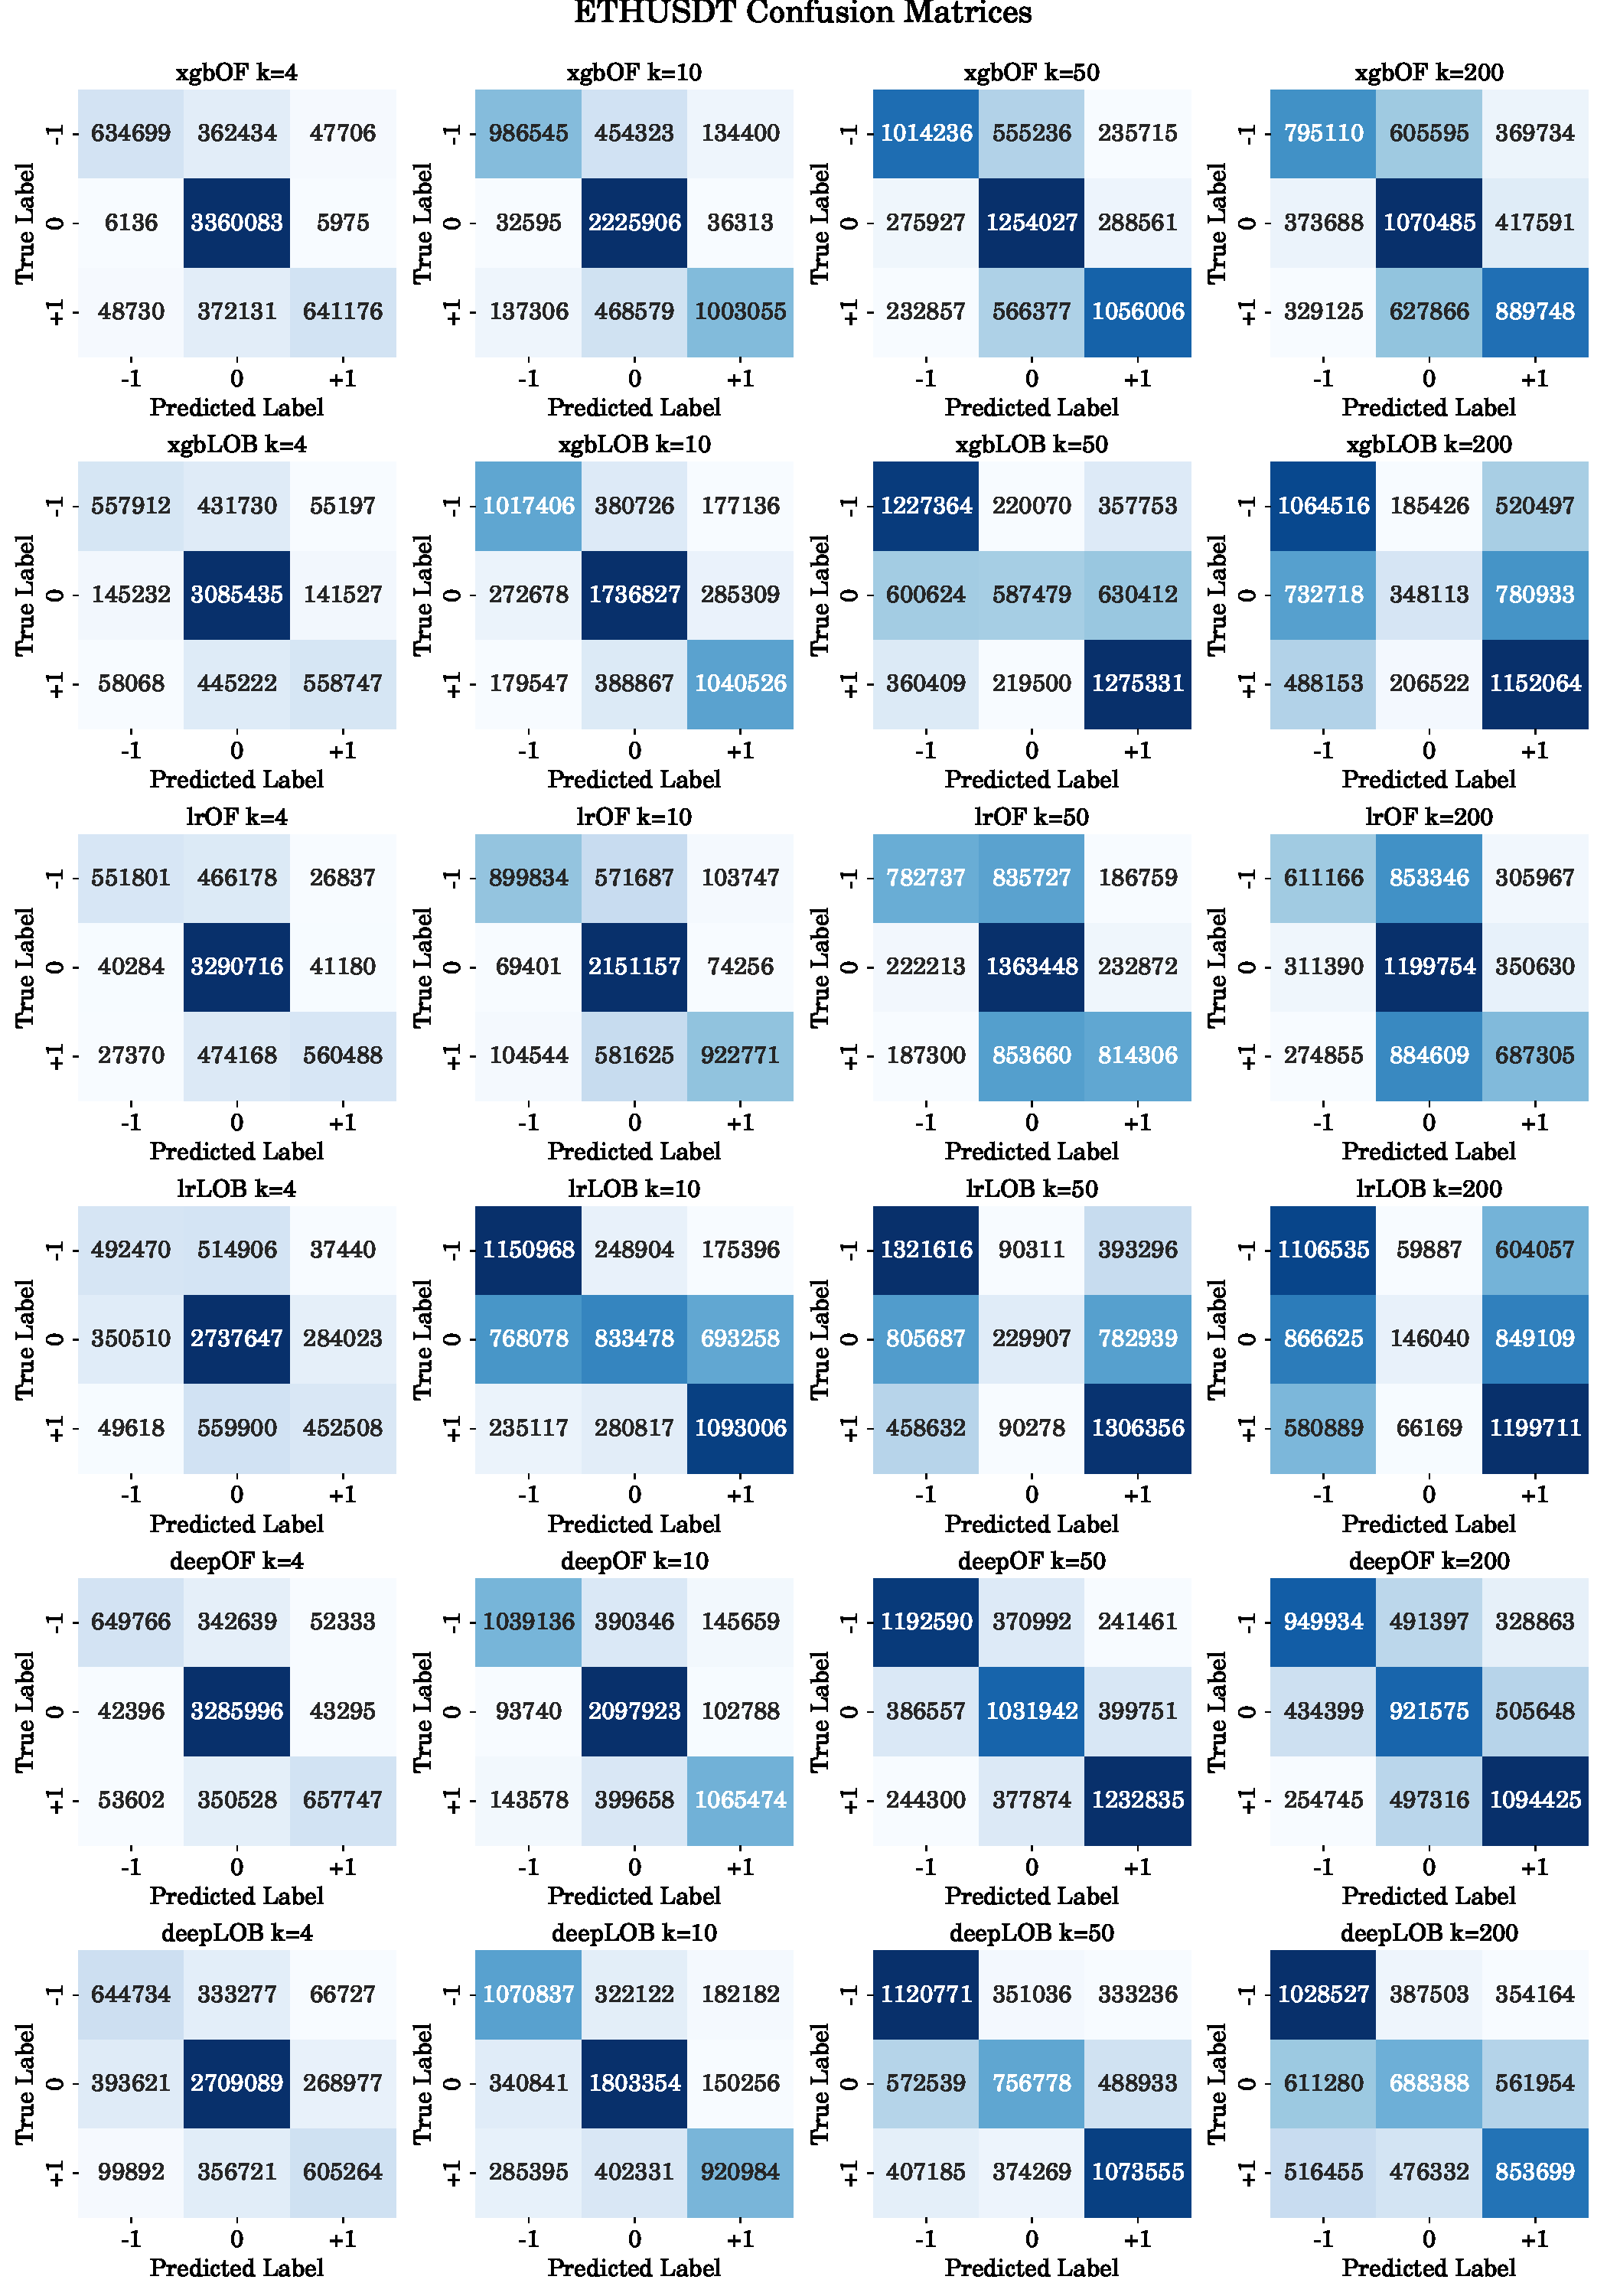
\includegraphics[width=1.0\textwidth]{./images/ETHUSDT_confusion_matrices.pdf}
    \caption{ETHUSDT confusion matrices. Note that counts are summed across windows.}
    \label{ETHUSDT_cm}
\end{figure}

\begin{figure}[htpb!]
    \centering
    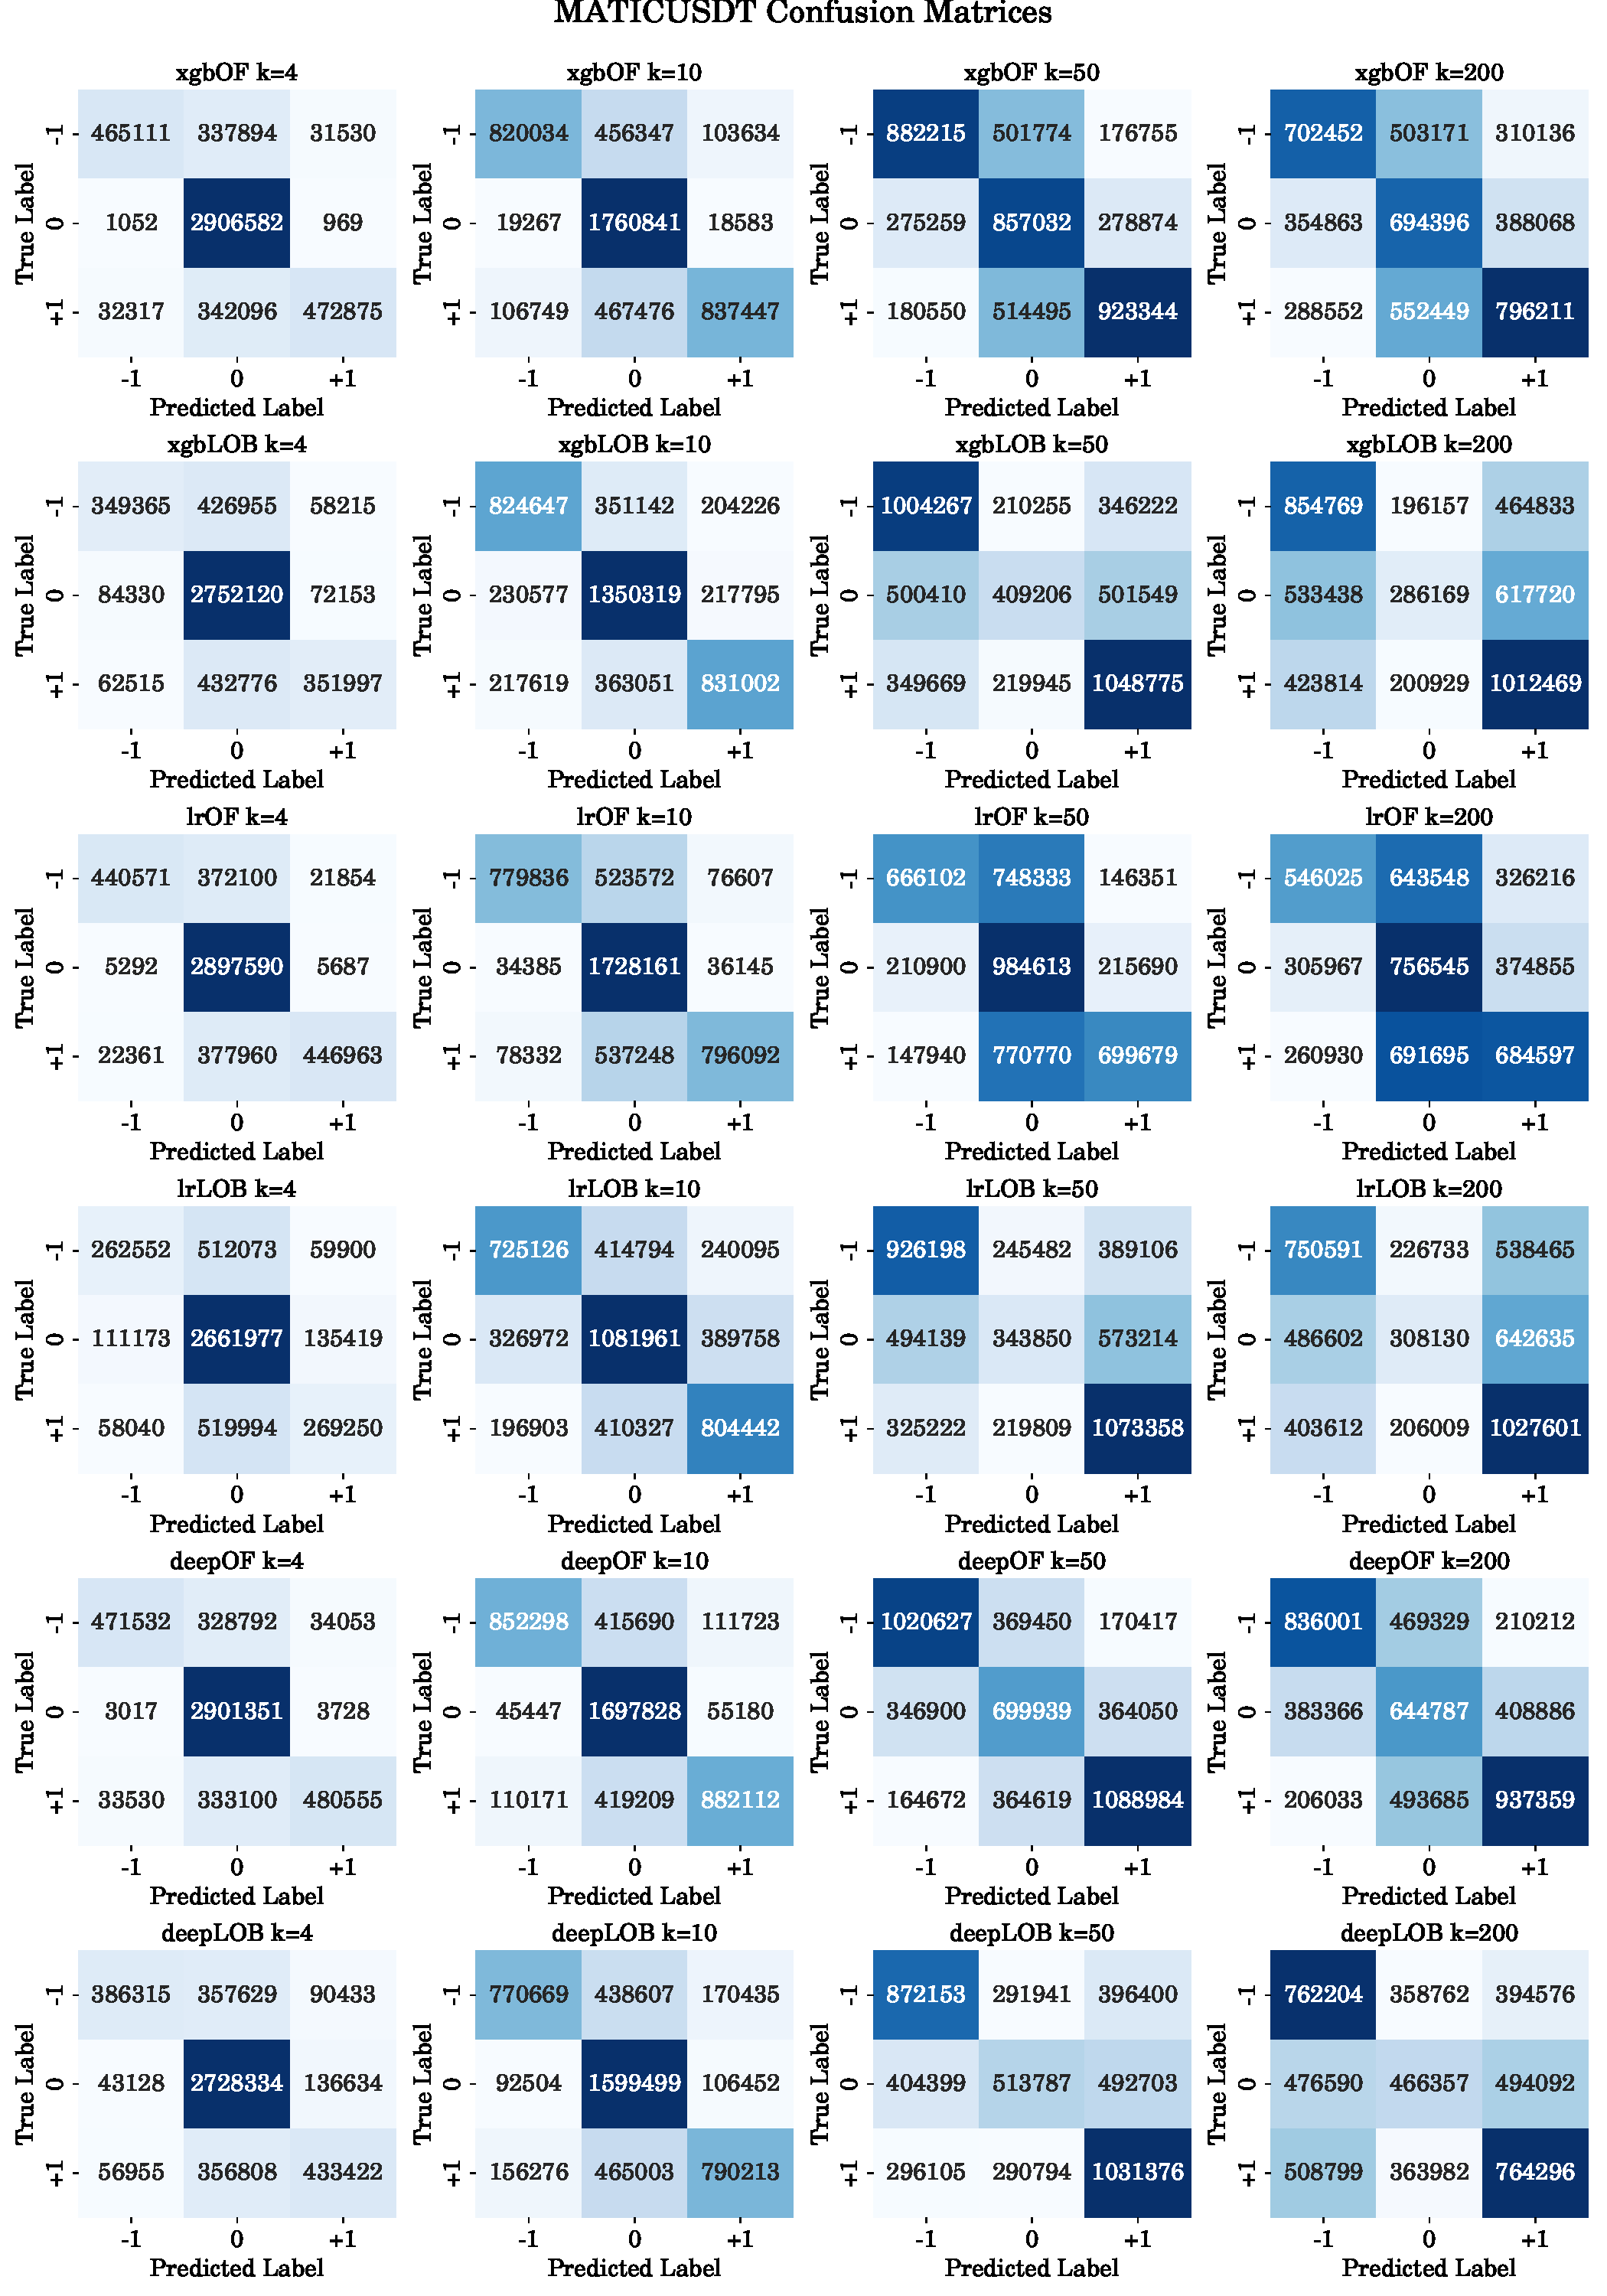
\includegraphics[width=1.0\textwidth]{./images/MATICUSDT_confusion_matrices.pdf}
    \caption{MATICUSDT confusion matrices. Note that counts are summed across windows.}
    \label{MATICUSDT_cm}
\end{figure}

\begin{figure}[htpb!]
    \centering
    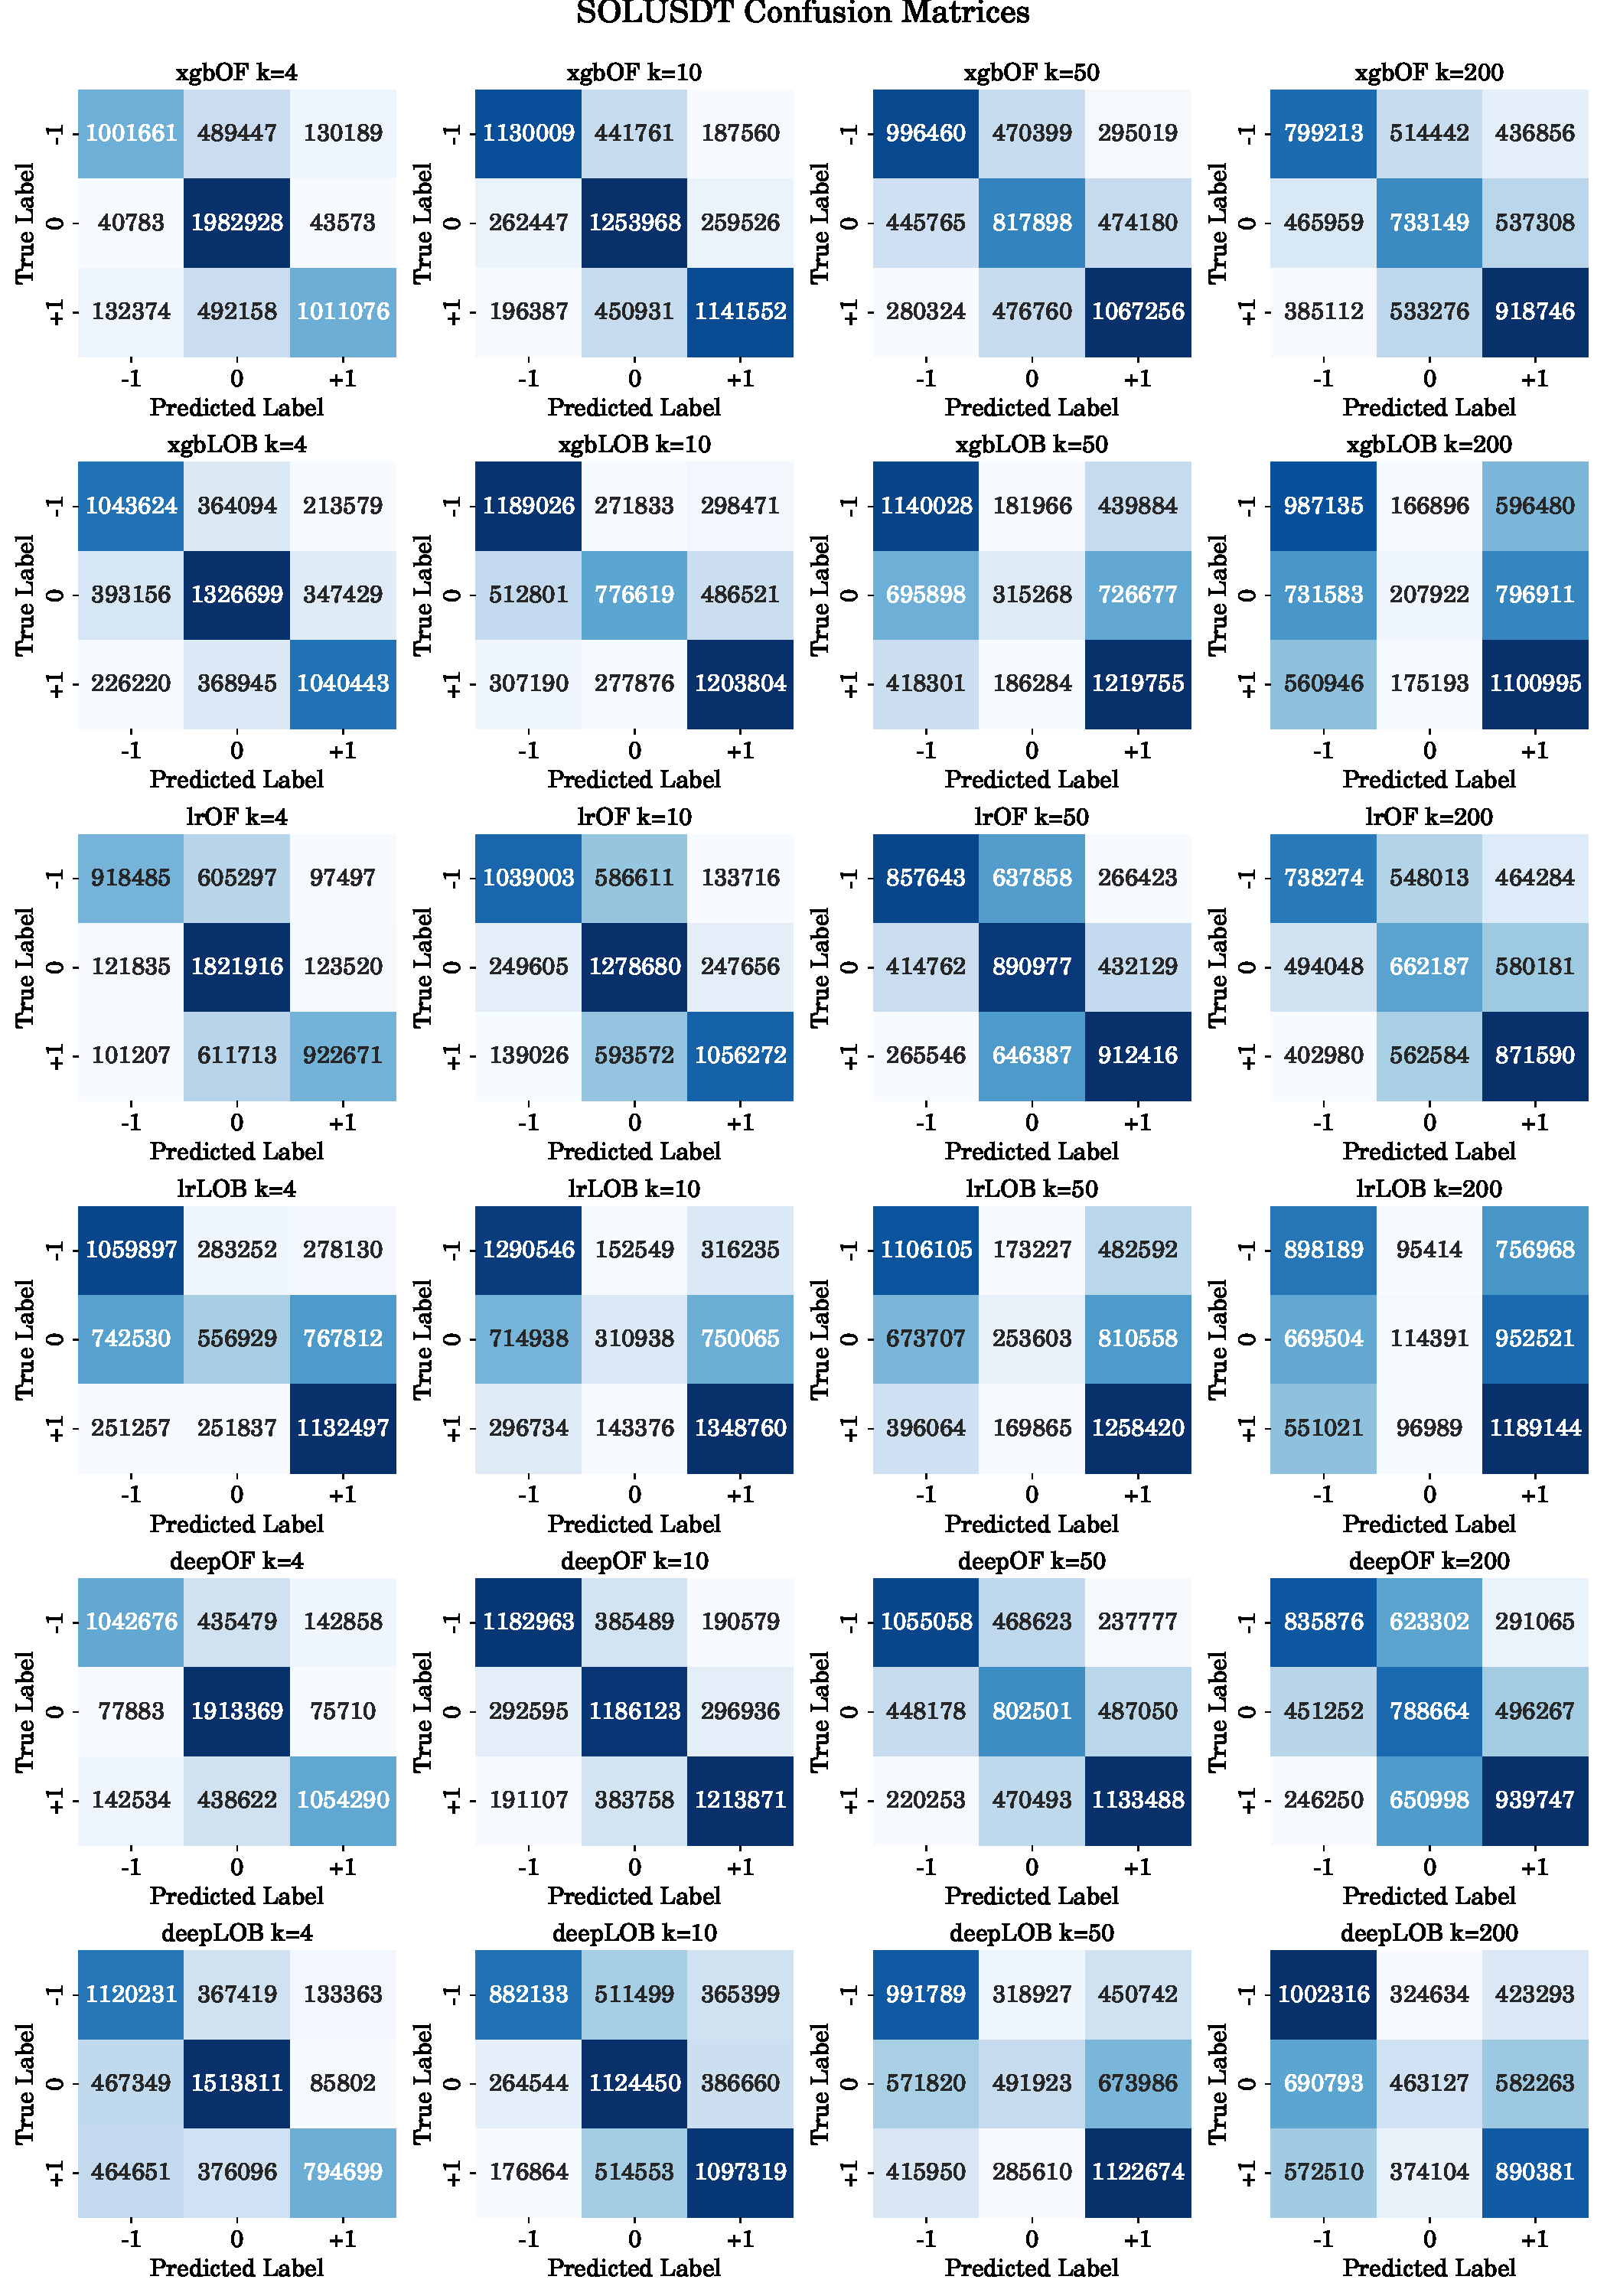
\includegraphics[width=1.0\textwidth]{./images/SOLUSDT_confusion_matrices.pdf}
    \caption{SOLUSDT confusion matrices. Note that counts are summed across windows.}
    \label{SOLUSDT_cm}
\end{figure}


\subsection{Feature Importances}
Another advantage of using a decision-tree-based model is that we get easily explainable
feature importances. During training, we split the tree at each level, using the feature
that gives us the best partition according to some metric. We can use this fact
to rank features based on the number of times a feature was used to split the tree. We
denote this count as the \textit{weight} of the feature.
More influential features will have a higher weight since they are the best discriminators
of the data.

We plot the top 10 LOB features for xgbLOB BTCUSDT in Figure \ref{top_10_lob_features} for different $k$, prediction horizons.
We see that for the LOB features, across all $k$, the highest weight features are 
the bid and ask quantities at the first level. This is very interesting,
and tells us that for the LOB model the top levels of the orderbook are the most relevant.
As we increase $k$, we start seeing larger lags being more important.  Recall that due to memory constraints
we set $T=\min(k, 20)$, so the maximum lag is 19. For $k > 20$ it seems
we would certainly benefit from a larger lookback.
Also a very important note; the majority of the top 10 features are quantity features. Recall
that the LOB features are both quantity and price. Clearly this shows that the model
is not using the price features effectively, and this demonstrates the need for a better
representation, such as orderflow.

We also plot the top 10 OF features for xgbOF BTCUSDT in Figure \ref{top_10_of_features}.
Again we see that the first level features are the most influential. This is good to see,
since it confirms the commonly shared idea that the top of the orderbook has the
most impact on price movement. Again we also see that, as we increase $k$, larger lag features
start to appear.

Next we examine the distribution of weights over all non-zero weighted features in Figures \ref{all_lob_features}
and \ref{all_of_features}. Instead of ordering the features by weight, we now order the features
by their index. Recall the LOB features are:
\begin{equation*}
    [\text{ask}\_\text{price}\_\ell\_\text{lag}\_p, \text{ask}\_\text{qty}\_\ell\_\text{lag}\_p, \text{bid}\_\text{price}\_\ell\_\text{lag}\_p, \text{bid}\_\text{qty}\_\ell\_\text{lag}\_p]_{\ell = 1, ..., 10, p = 0, ..., T}
\end{equation*}
And the OF features are:
\begin{equation*}
    [\text{ask}\_\text{orderflow}\_\ell\_\text{lag}\_p, \text{bid}\_\text{orderflow}\_\ell\_\text{lag}\_p]_{\ell = 1, ..., 10, p = 0, ..., T}
\end{equation*}
Where $\ell$ indexes the orderbook level, and $p$ indexes the lag.
Note that in Figures \ref{all_lob_features} and \ref{all_of_features} we distinguish different feature groups using different colors.
Each color represent a unique (feature type, lag) pair, where feature type is either quantity or price for LOB and orderflow for OF.
So for example, the first color represents all price features with lag 0. This allows us to compare feature weights
for price vs. quantity features and also for different lags. Also since features are ordered by index, we can compare
feature weights across levels, e.g. the first bar in a color group represents the first level for that feature type and lag.

Firstly we note that in \ref{all_lob_features} only every other bar has significant weight. These bars are quantity features and
the price features have very small, often zero, weight for most levels and lags.
This shows that the model is hardly using the price features, further confirming
the inefficiency of the LOB representation. For both the OF representation and LOB representation we see that for each color the feature weights
are decreasing as we increase the feature index. This shows that the features at the top levels have highest weight, and evidences
the idea that deeper levels are less relevant for mid-price prediction.
We also see that the first few levels all have similar weight across colors. This shows that the first few levels of the orderbook
are roughly equally important across lags. For example, ask\_qty\_1\_lag\_9 has similar importance to ask\_qty\_1\_lag\_0. So we see
that using auto-regressive (lagged) features is important, but using deeper levels of the orderbook is less important.

Note that we do not distinguish between ask and bid features because we find them to be equally important.

\begin{figure}[htpb!]
    \centering
    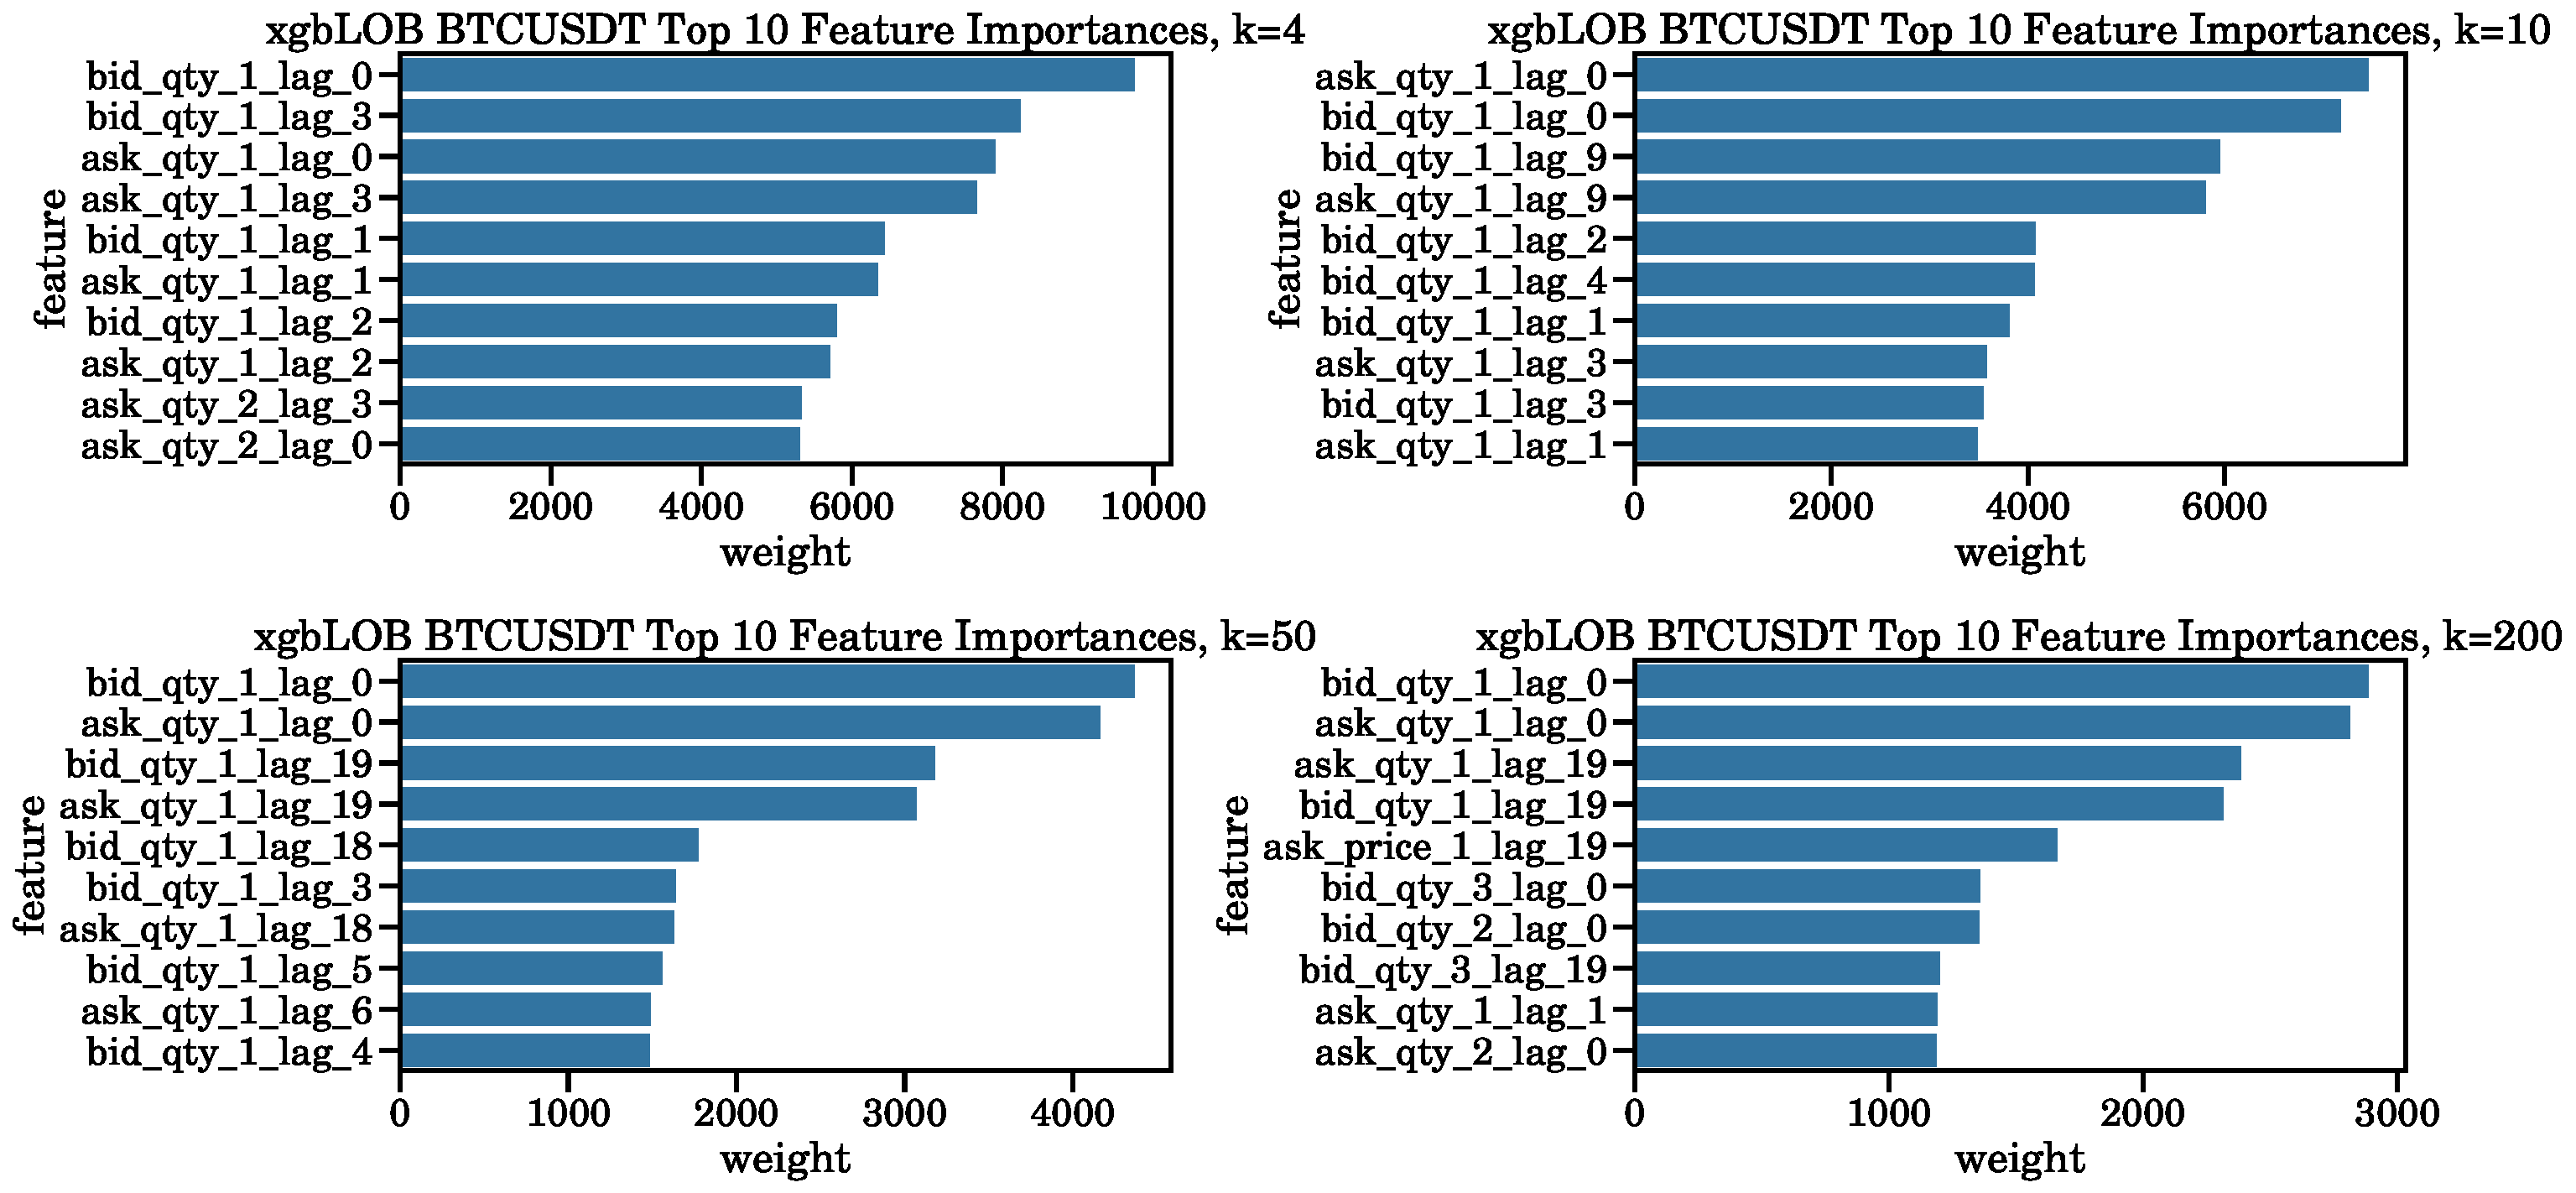
\includegraphics[width=1.0\textwidth]{./images/xgboost_LOB_BTCUSDT_top_10_feature_importances.pdf}
    \caption{Top 10 XGBoost LOB Feature Importances for BTCUSDT, measured by weight = number of times a feature was split on.}
    \label{top_10_lob_features}
\end{figure}
\begin{figure}[htpb!]
    \centering
    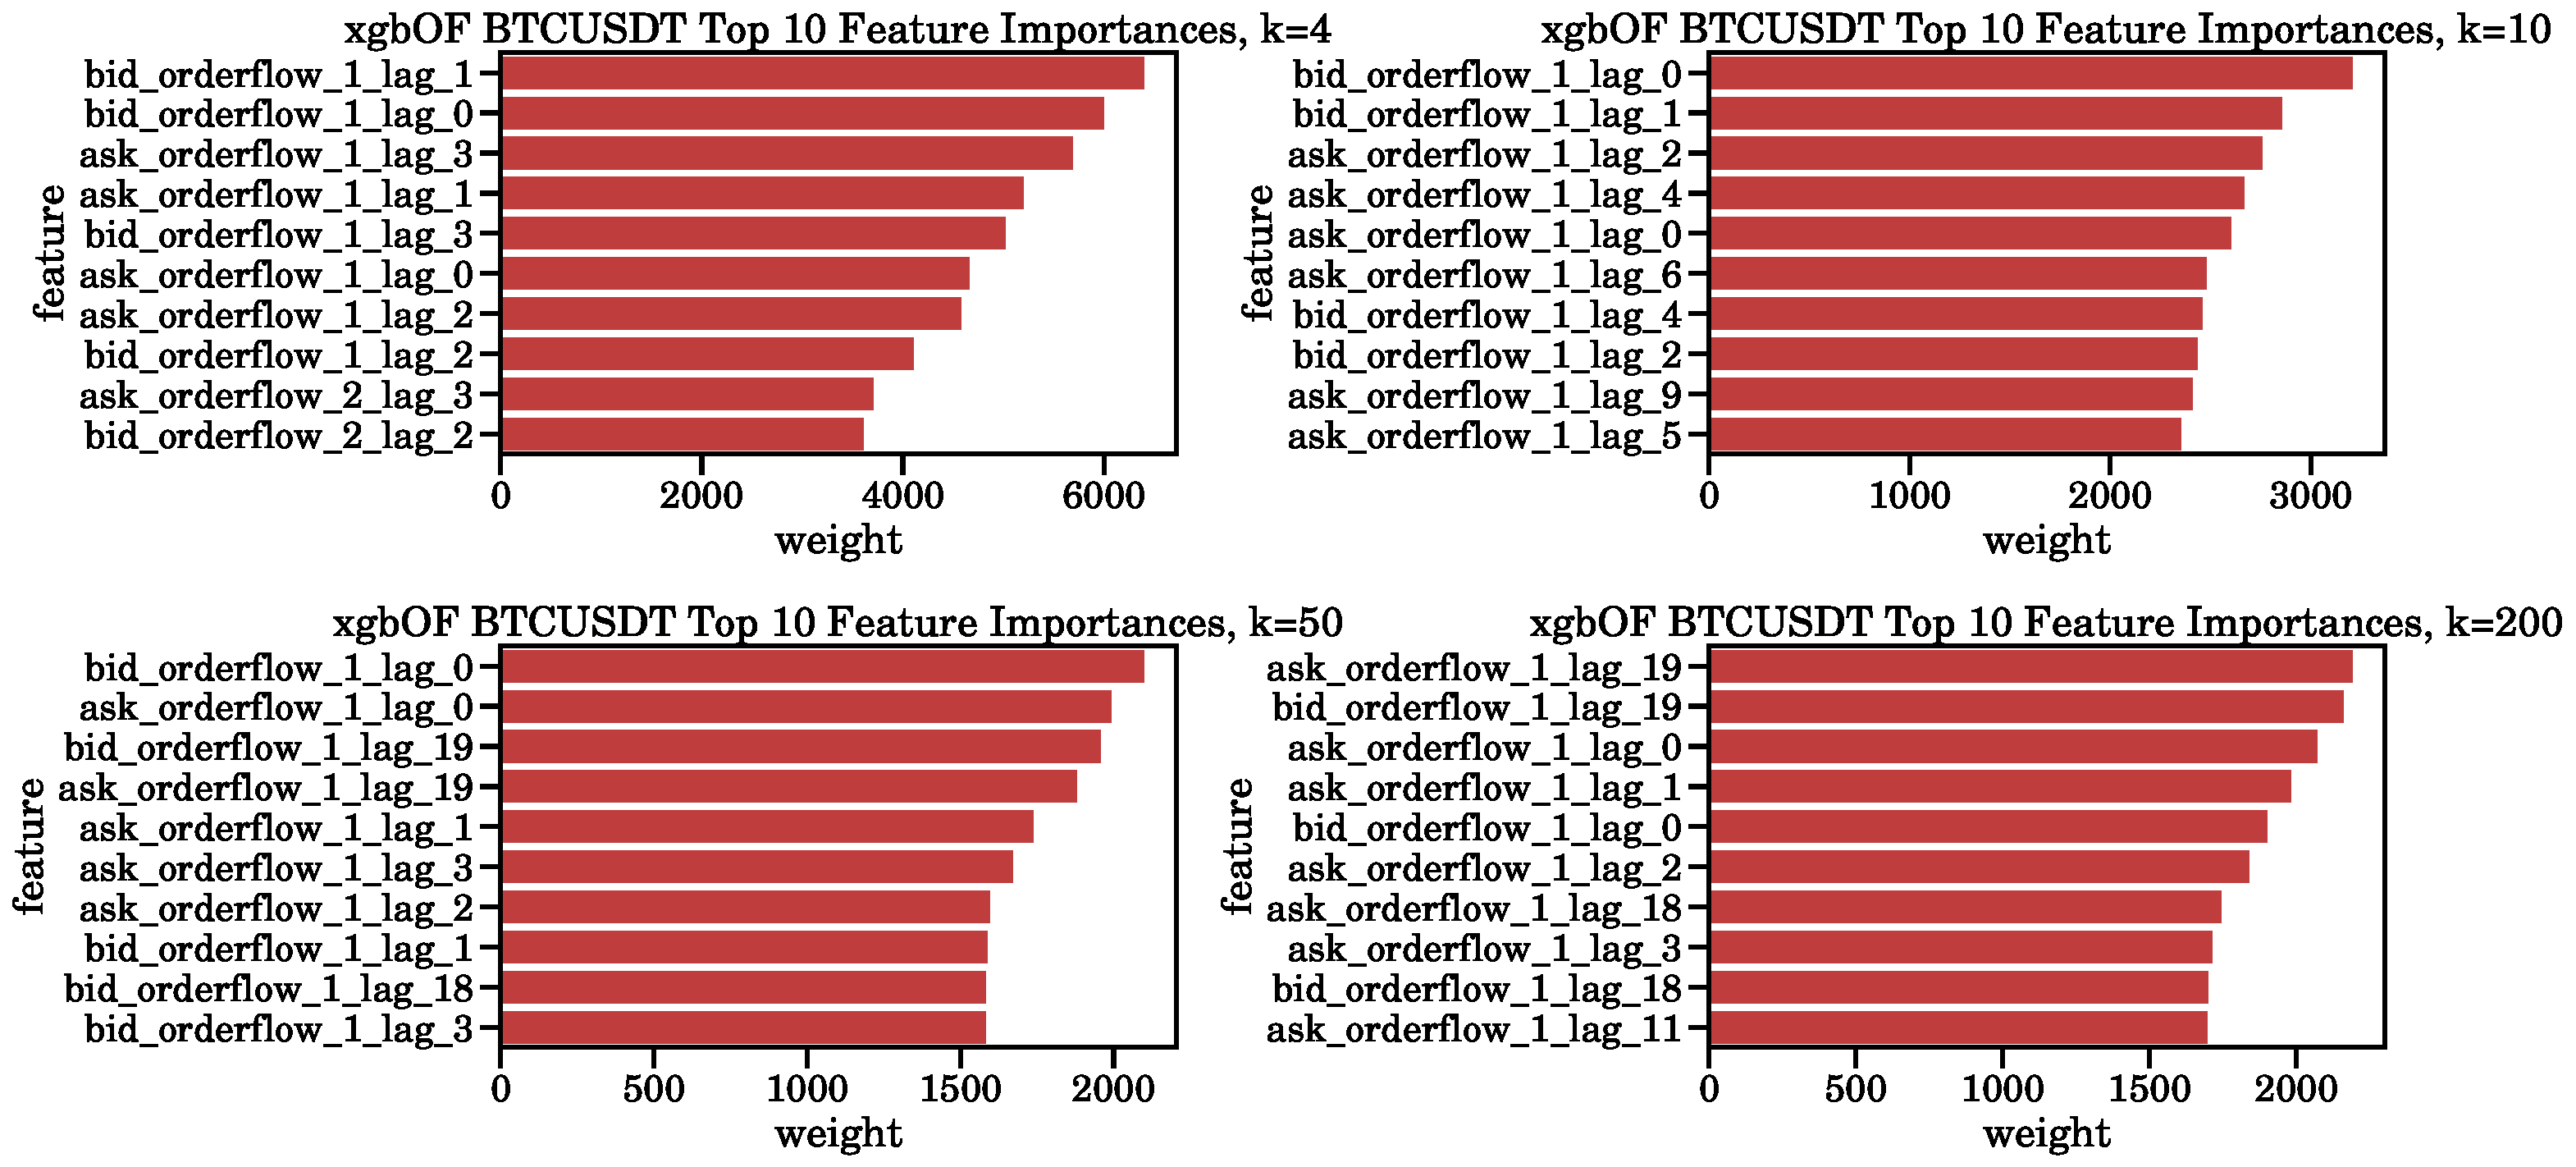
\includegraphics[width=1.0\textwidth]{./images/xgboost_OF_BTCUSDT_top_10_feature_importances.pdf}
    \caption{Top 10 XGBoost OF Feature Importances for BTCUSDT, measured by weight = number of times a feature was split on.}
    \label{top_10_of_features}
\end{figure}


\begin{figure}[htpb!]
    \centering
    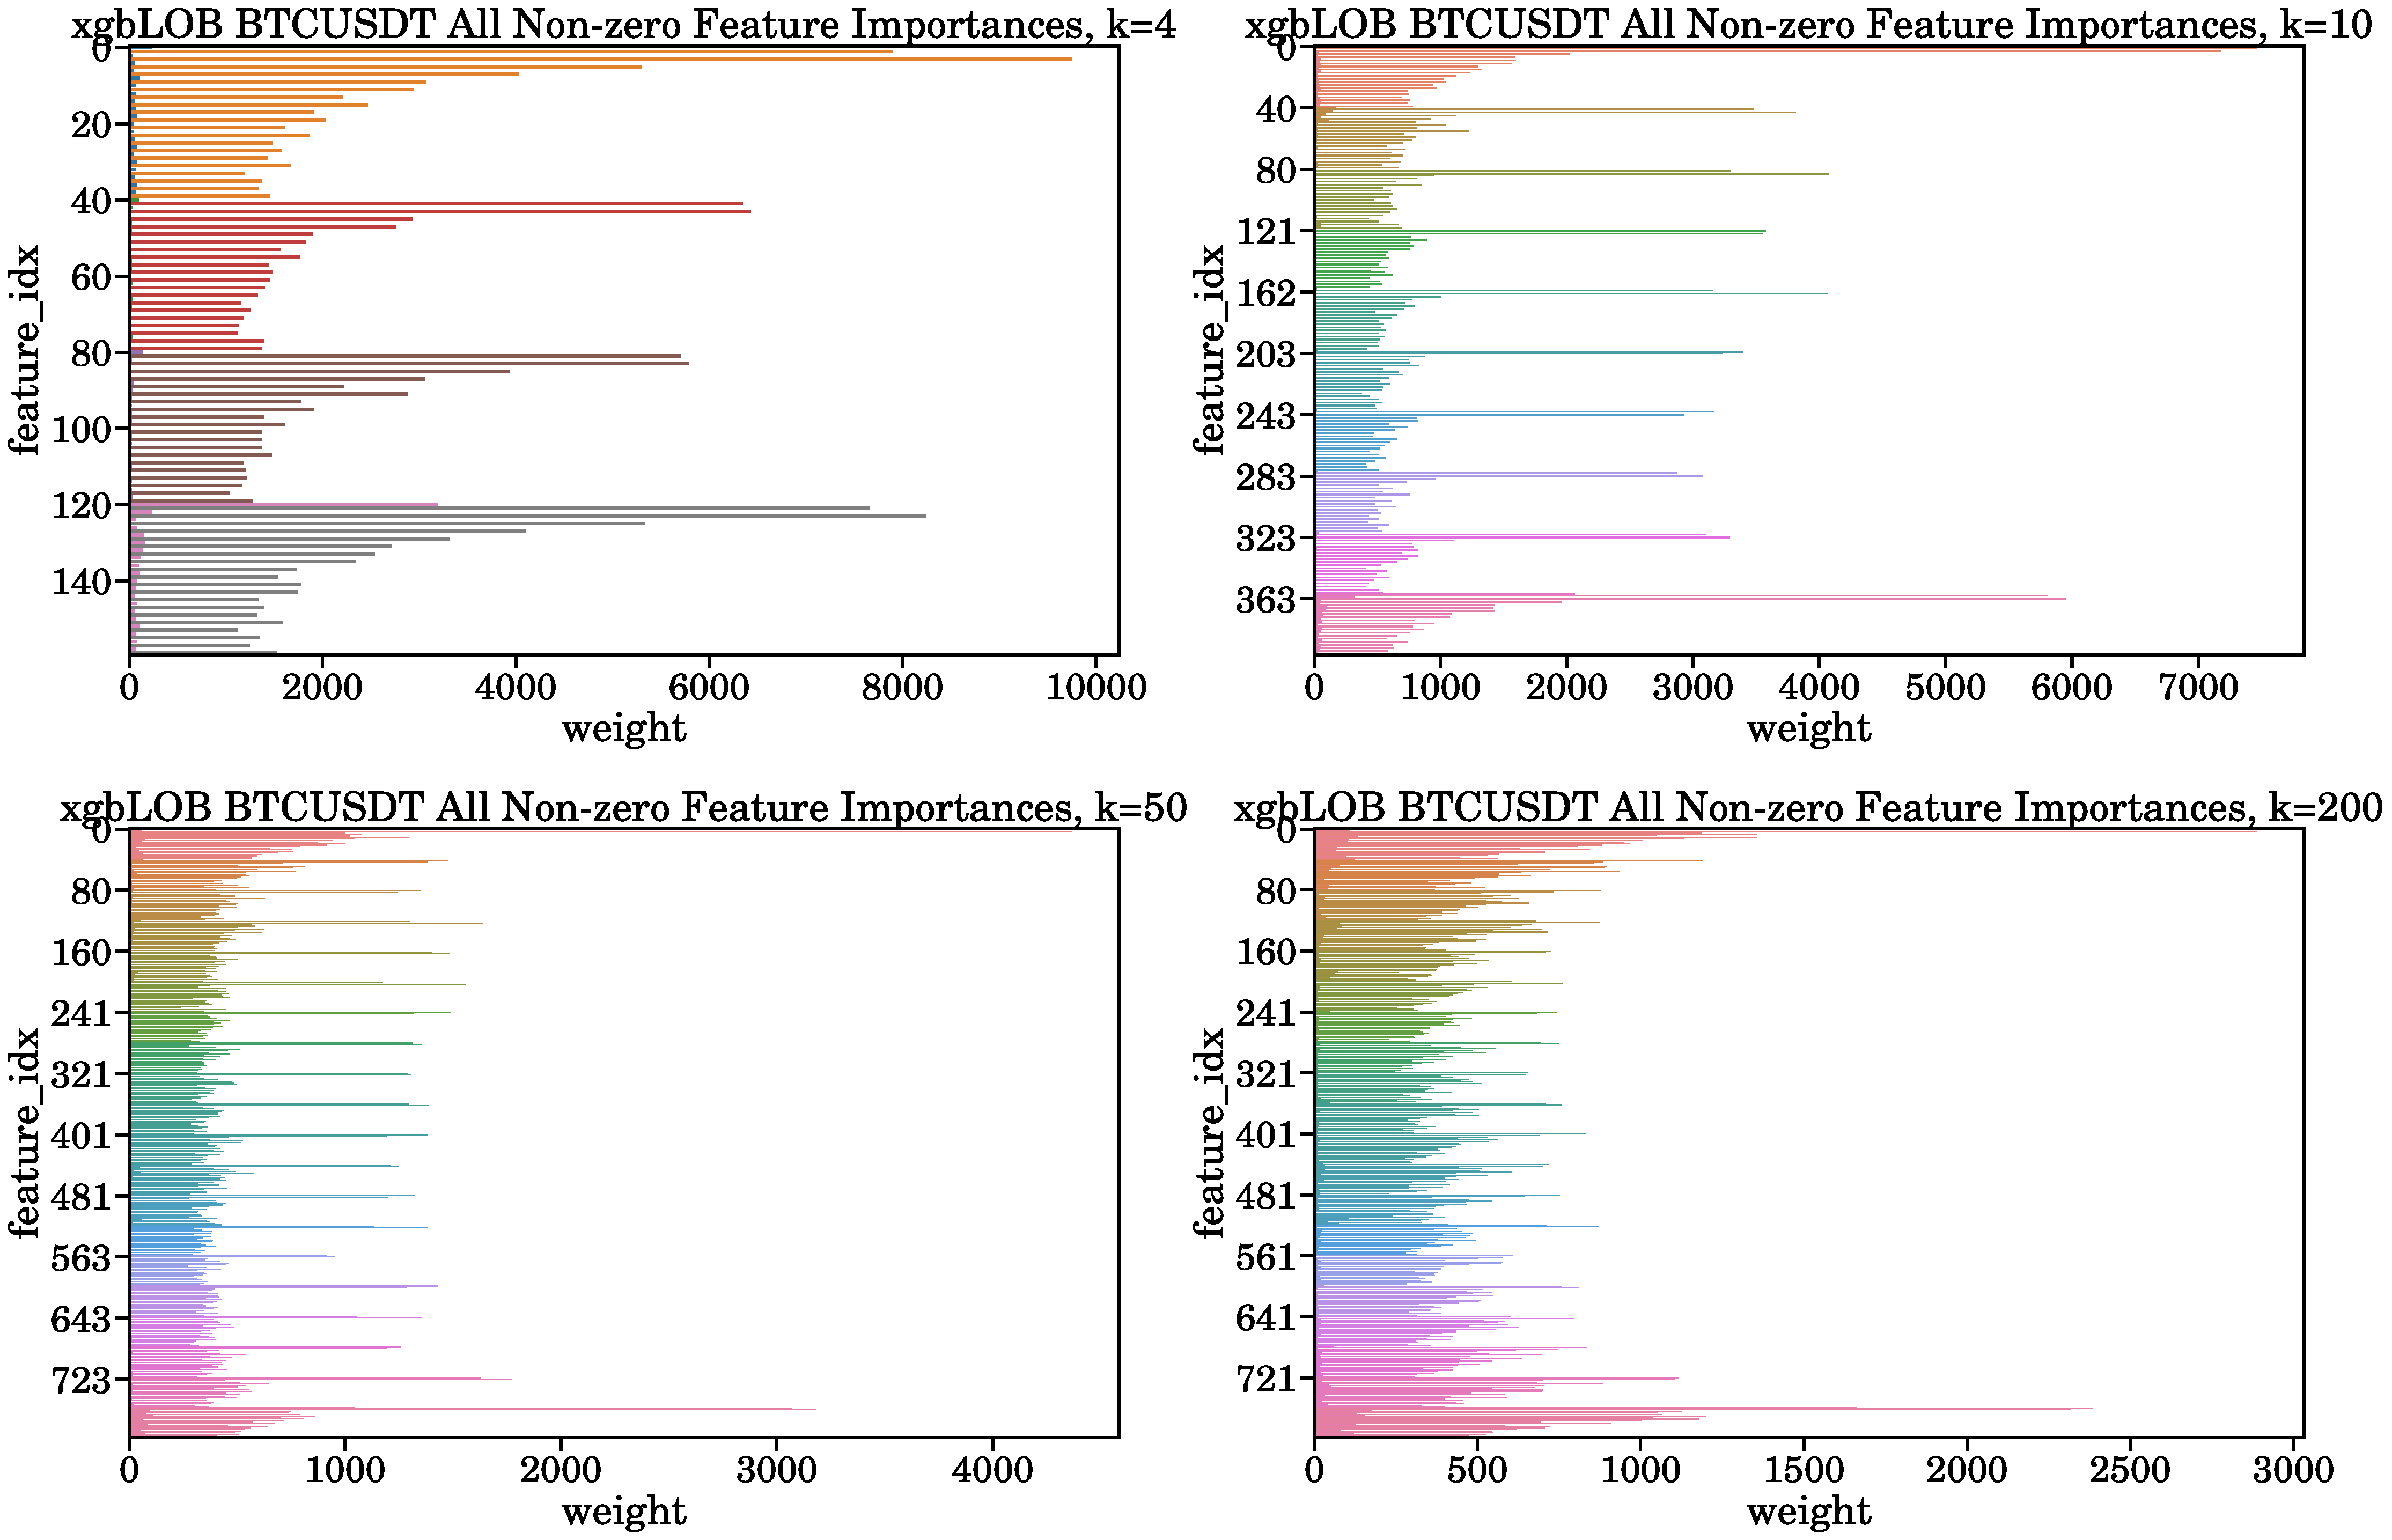
\includegraphics[width=0.9\textwidth]{./images/xgboost_LOB_BTCUSDT_all_feature_importances.pdf}
    \caption{All non-zero LOB feature importances for BTCUSDT, measured by weight = number of times a feature was split on.
    Note that the colors represent unique (feature type, lag) pairs, where feature type is either quantity or price and lag $\in \{0, ..., T\} $,
    e.g. the first color represents price features with lag 0.}
    \label{all_lob_features}
\end{figure}

\begin{figure}[htpb!]
    \centering
    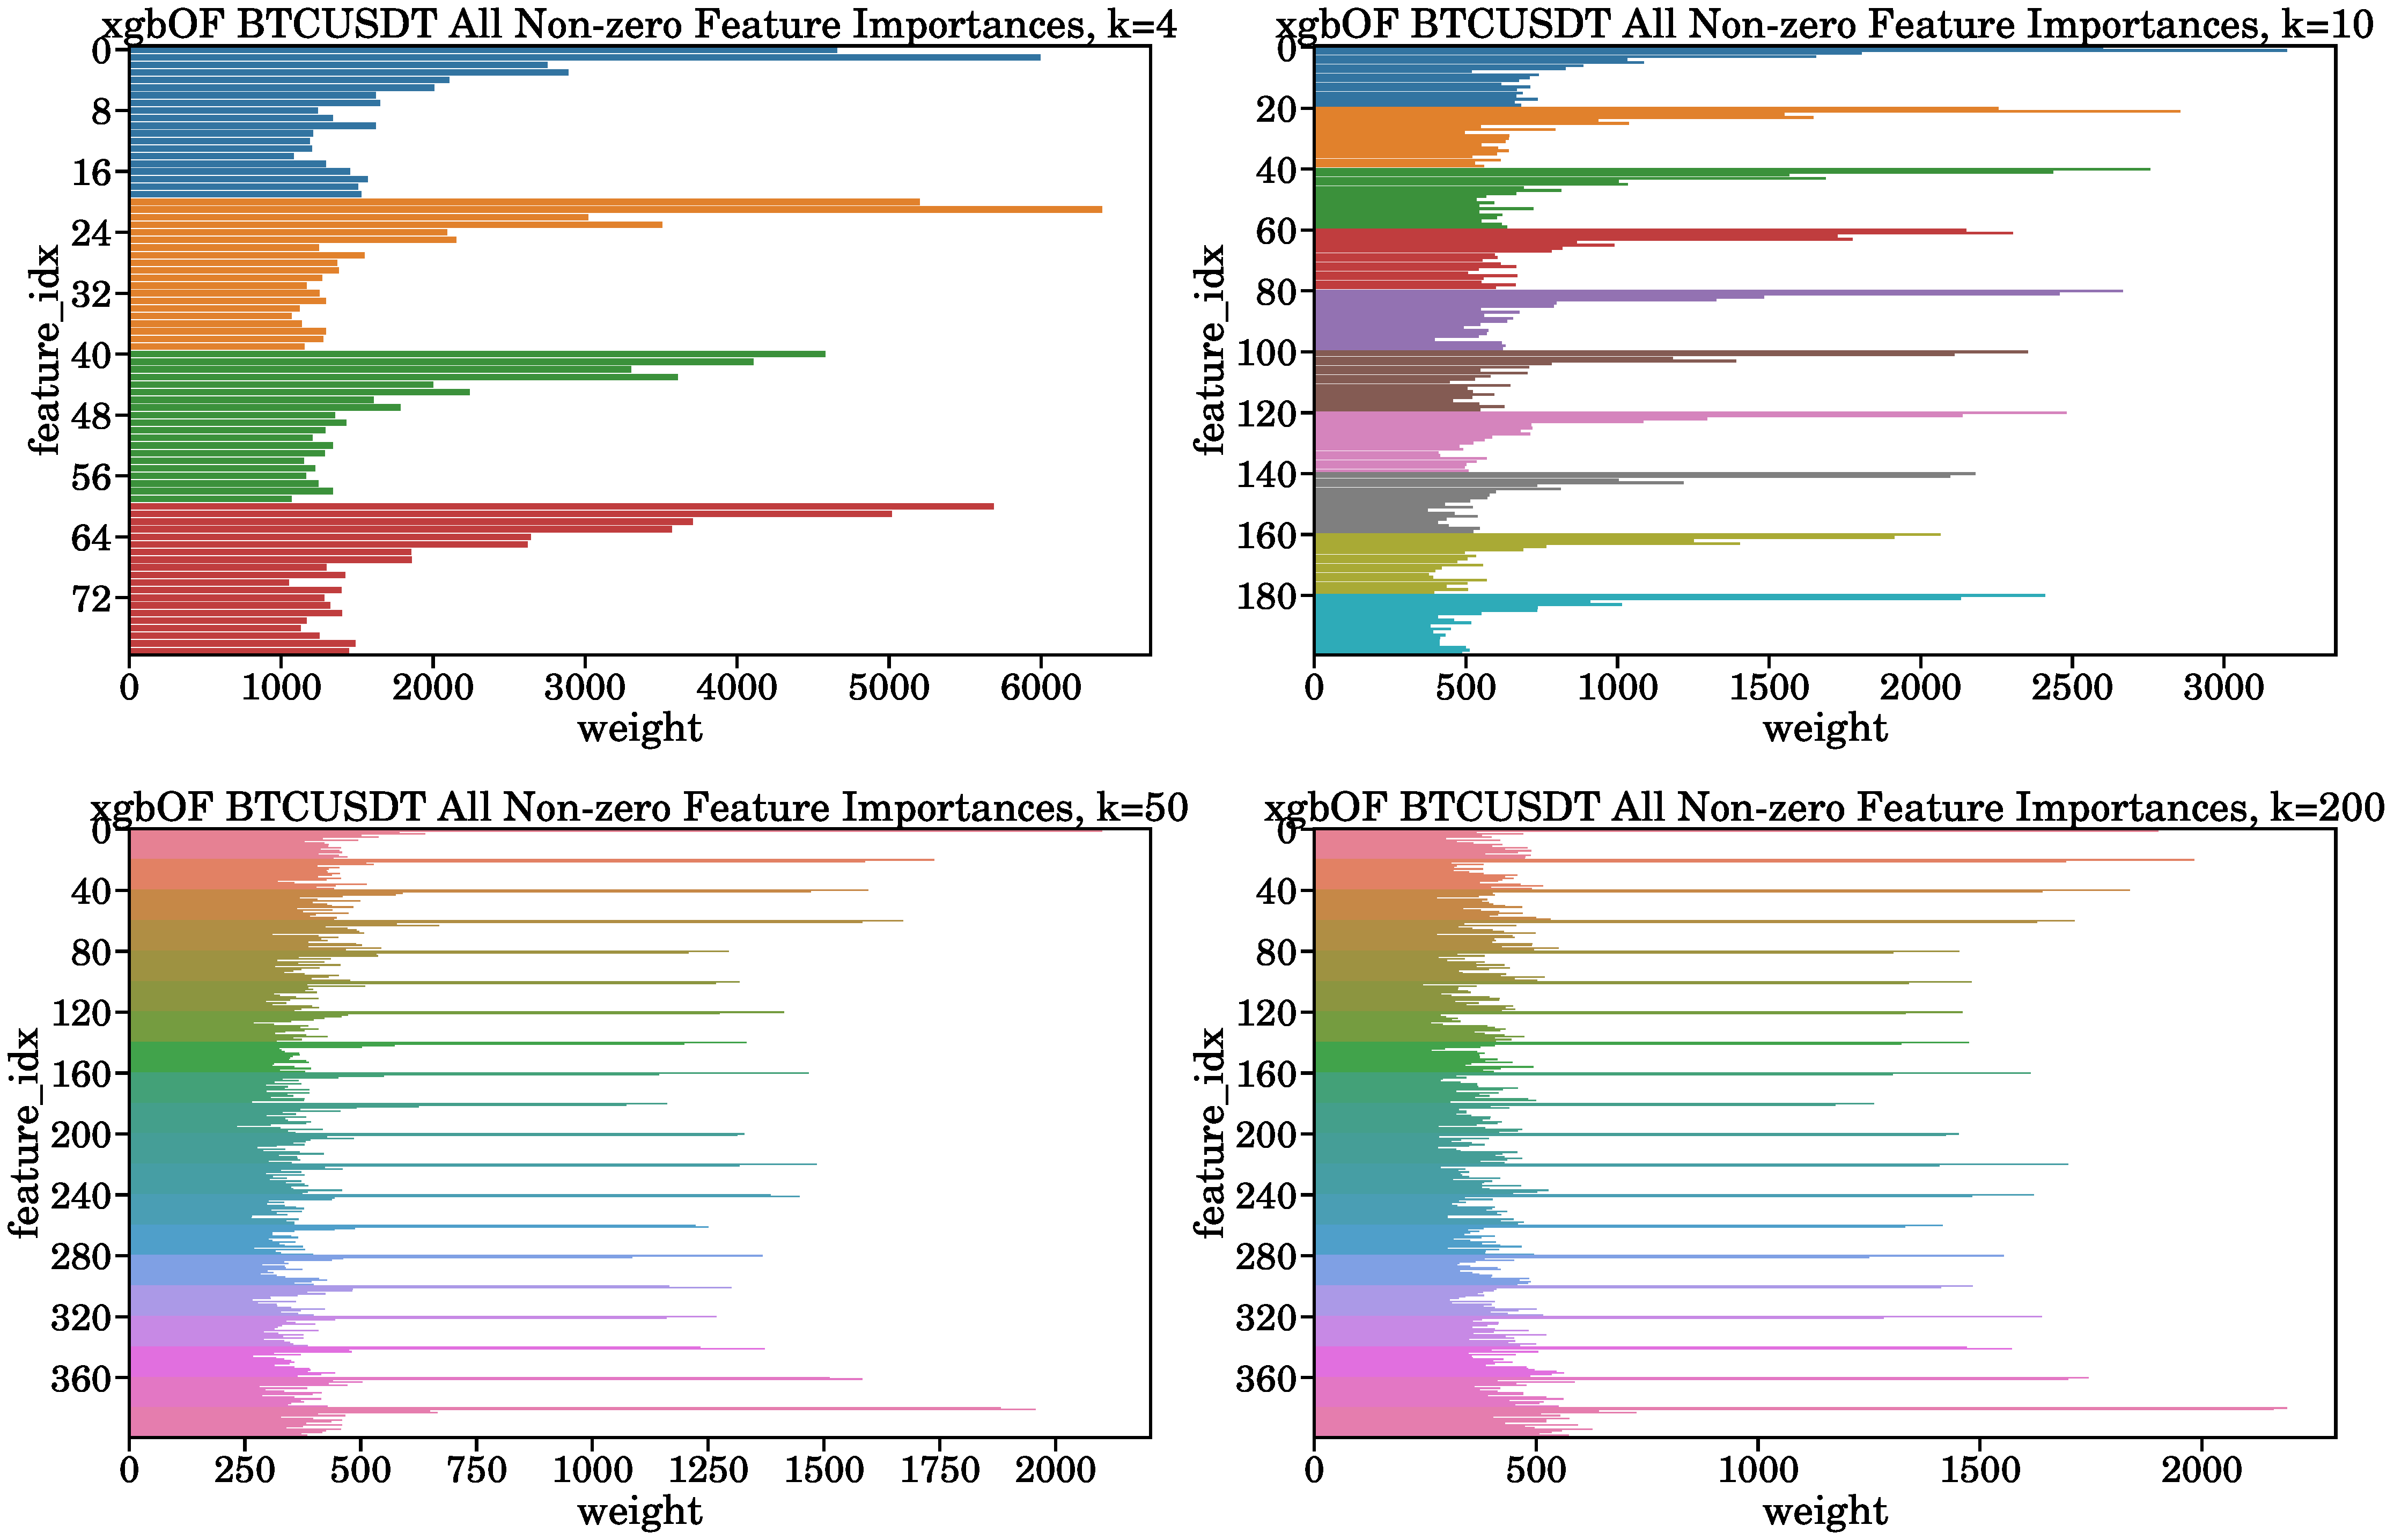
\includegraphics[width=0.9\textwidth]{./images/xgboost_OF_BTCUSDT_all_feature_importances.pdf}
    \caption{All non-zero OF feature importances for BTCUSDT, measured by weight = number of times a feature was split on.
    Note that the colors represent unique lags, where lag $\in \{0, ..., T\} $. 
    E.g. the first color represents all features with lag 0.}
    \label{all_of_features}
\end{figure}

\subsection{Modelling Recommendations}
To conclude, we recommend the xgbOF model for shorter time horizons due its superior performance,
ease of use, interpretability, scalability and lower training time.
This is interesting since, to our knowledge, XGBoost is not mentioned in the literature for high frequency orderbook mid-price prediction.
It would be interesting to see how the xgbOF model compares with the models presented in \cite{ZHANG2019}, \cite{KOLM2023} and \cite{LUCCHESE2024} when trained on their data.


For longer time horizons deepOF was the clear winner. Whether this was due to superior ability to capture long term
temporal dependencies or the fact that our xgbOF had a cap on lookback due to memory constraints remains to be seen
and we recommend anyone looking to predict mid-prices at longer time horizons to try both models.


\chapter{Conclusion}
\hrule
\vspace{40pt}

\section{Summary}
In this paper we explored various machine learning models for predicting high frequency returns
for four of the main cryptocurrency futures trading pairs, BTCUSDT, ETHUSDT, MATICUSDT and SOLUSDT. 
We constructed a novel data set from a live WebSocket stream from Binance, the worlds largest centralized cryptocurrency exchange.
Following \cite{CONT2013}, we defined a stationary transformation of the raw orderbook data called orderflow, 
and motivated its definition by showing that under a stylized model of the orderbook, orderflow can be used to measure linear price impact
of orderbook events. We then defined our modelling objective as a three-class classification problem, predicting the direction of the smoothed
mid-price returns for several prediction horizons. For this task, we introduced several traditional machine learning and also deep learning
models that use either the orderflow representation or the raw orderbook representation. Specifically, from traditional ML we introduced
Logistic Regression and XGBoost models. For our deep learning models, we used the deepLOB model from \cite{ZHANG2019} and the deepOF model
from \cite{KOLM2023} which use the raw orderbook/orderflow representations respectively.
We trained, validated and tested our models for each trading pair and multiple prediction horizons on 8 windows from 05-02-2024 to 25-02-2024.
We presented the results on the test set and also evaluated the feature importances for each XGBoost model.

\section{Conclusions}
From our results section we showed that we can predict the direction of smoothed mid-price returns at 
multiple short term time horizons for our Binance WebSocket data with good performance.
We also saw that the price features are not significantly used and we concluded that the orderflow representation is far superior
to the raw orderbook data representation for this task. This agrees with the findings of \cite{KOLM2023}.
We found that simpler traditional machine learning models have very competitive performance when compared with the much larger
and more complex deep learning models. This is a significant result, since it challenges the idea that we need a large and complicated
deep learning model to achieve state of the art performance for orderbook prediction. \cite{ZHANG2019}, \cite{KOLM2023}, \cite{LUCCHESE2024}.
This is very good news for practical application, since simpler models are much more explainable, which is a very important quality
for many quantitative applications.

\section{Future Work}
As previously mentioned, it would be interesting to see how our models compare with those found in \cite{ZHANG2019}, \cite{KOLM2023}, \cite{LUCCHESE2024} when applied to their data.

Also, in this paper we only explored 4 trading pairs, when in fact Binance has over two-hundred perpetual futures trading pairs available.
It would be interesting to apply the same methodology presented in this paper to a larger group of trading pairs and explore
the differences across pairs.

A major advantage of using the Binance WebSocket data is that it is freely available and live at any time. Our next steps
would be to adapt the models presented here to be, \textit{online}, i.e. continously learning and adapting in real time.
Then we could continuously test the models in real time for a longer period of time. This would show definitively
whether this methodology is practical for real world trading applications.





\appendix

\chapter{Extended Classification Results}
\hrule
Here we present the results for each symbol, for each $k$, for each model, averaged across windows.
We give standard deviations in parenthesis. For each metric we have an array of $3$ values, where the first
value represent the metric for class $-1$, the second class $0$ and the third class $+1$.
\begin{table}[htbp!] 
\resizebox{0.99\textwidth}{!}{
\begin{tabular}{llllll}
\toprule
accuracy & precision & recall & f1-score & support & model \\
\midrule
0.87(0.03) & [0.94 0.84 0.95]([0.03 0.04 0.03]) & [0.61 1.   0.6 ]([0.01 0.   0.02]) & [0.74 0.91 0.74]([0.01 0.03 0.01]) & [111278 421391 114625]([32887 38390 34515]) & xgbOF \\
0.79(0.04) & [0.71 0.81 0.72]([0.08 0.05 0.09]) & [0.59 0.89 0.56]([0.06 0.06 0.05]) & [0.64 0.85 0.62]([0.02 0.04 0.03]) & [111278 421391 114625]([32887 38390 34515]) & xgbLOB \\
0.84(0.04) & [0.9  0.82 0.9 ]([0.02 0.06 0.01]) & [0.57 0.98 0.56]([0.02 0.01 0.01]) & [0.69 0.89 0.69]([0.01 0.04 0.01]) & [111277 421386 114625]([32887 38390 34515]) & lrOF \\
0.69(0.07) & [0.61 0.78 0.6 ]([0.16 0.09 0.16]) & [0.51 0.8  0.5 ]([0.18 0.19 0.18]) & [0.5  0.76 0.5 ]([0.08 0.1  0.09]) & [111277 421386 114625]([32887 38390 34515]) & lrLOB \\
0.86(0.03) & [0.9  0.84 0.91]([0.03 0.04 0.02]) & [0.62 0.98 0.62]([0.02 0.01 0.02]) & [0.74 0.91 0.73]([0.01 0.02 0.01]) & [111258 421321 114619]([32882 38387 34517]) & deepOF \\
0.75(0.2) & [0.7  0.74 0.76]([0.2  0.28 0.21]) & [0.69 0.8  0.62]([0.11 0.31 0.11]) & [0.66 0.77 0.65]([0.09 0.3  0.11]) & [111258 421321 114619]([32882 38387 34517]) & deepLOB \\
\bottomrule
\end{tabular}

}\caption{Mean class-wise BTCUSDT test set classification results across windows for $k=4$. \\(Standard deviations are given in parenthesis) Note that the class ordering is [-1, 0, 1].}
\end{table}
\begin{table}[htbp!] 
\resizebox{0.99\textwidth}{!}{
\begin{tabular}{llllll}
\toprule
accuracy & precision & recall & f1-score & support & model \\
\midrule
0.8(0.03) & [0.9  0.72 0.91]([0.03 0.06 0.03]) & [0.64 0.99 0.63]([0.02 0.   0.02]) & [0.75 0.84 0.74]([0.01 0.04 0.  ]) & [176543 286661 184084]([41637 55324 43785]) & xgbOF \\
0.72(0.02) & [0.7  0.73 0.7 ]([0.06 0.07 0.06]) & [0.69 0.74 0.7 ]([0.04 0.07 0.03]) & [0.7  0.73 0.7 ]([0.02 0.05 0.02]) & [176543 286661 184084]([41637 55324 43785]) & xgbLOB \\
0.76(0.04) & [0.86 0.69 0.87]([0.02 0.08 0.02]) & [0.6  0.96 0.6 ]([0.01 0.01 0.01]) & [0.71 0.8  0.71]([0.01 0.05 0.01]) & [176543 286661 184084]([41637 55324 43785]) & lrOF \\
0.58(0.07) & [0.59 0.7  0.59]([0.13 0.12 0.13]) & [0.73 0.43 0.72]([0.14 0.26 0.14]) & [0.62 0.46 0.62]([0.06 0.18 0.07]) & [176543 286661 184084]([41637 55324 43785]) & lrLOB \\
0.79(0.03) & [0.85 0.74 0.85]([0.01 0.06 0.02]) & [0.67 0.94 0.67]([0.01 0.02 0.02]) & [0.75 0.83 0.75]([0.01 0.04 0.01]) & [176510 286617 184072]([41631 55319 43788]) & deepOF \\
0.74(0.06) & [0.77 0.73 0.8 ]([0.1  0.06 0.02]) & [0.66 0.87 0.61]([0.11 0.09 0.11]) & [0.69 0.79 0.68]([0.05 0.06 0.08]) & [176510 286617 184072]([41631 55319 43788]) & deepLOB \\
\bottomrule
\end{tabular}

}\caption{Mean class-wise BTCUSDT test set classification results across windows for $k=10$. \\(Standard deviations are given in parenthesis) Note that the class ordering is [-1, 0, 1].}
\end{table}
\begin{table}[htbp!] 
\resizebox{0.99\textwidth}{!}{
\begin{tabular}{llllll}
\toprule
accuracy & precision & recall & f1-score & support & model \\
\midrule
0.64(0.04) & [0.7  0.56 0.7 ]([0.02 0.1  0.03]) & [0.57 0.73 0.57]([0.03 0.07 0.03]) & [0.62 0.63 0.62]([0.02 0.09 0.03]) & [199331 238186 209760]([46599 66246 48099]) & xgbOF \\
0.56(0.04) & [0.55 0.6  0.55]([0.08 0.09 0.08]) & [0.72 0.27 0.73]([0.05 0.17 0.03]) & [0.62 0.34 0.62]([0.04 0.18 0.05]) & [199331 238186 209760]([46599 66246 48099]) & xgbLOB \\
0.57(0.05) & [0.68 0.49 0.69]([0.02 0.12 0.03]) & [0.43 0.79 0.44]([0.02 0.05 0.03]) & [0.53 0.6  0.53]([0.02 0.1  0.03]) & [199338 238189 209762]([46601 66248 48098]) & lrOF \\
0.51(0.06) & [0.51 0.53 0.52]([0.08 0.13 0.09]) & [0.72 0.16 0.74]([0.08 0.15 0.07]) & [0.59 0.2  0.6 ]([0.05 0.15 0.05]) & [199338 238189 209762]([46601 66248 48098]) & lrLOB \\
0.66(0.03) & [0.67 0.62 0.66]([0.02 0.09 0.03]) & [0.66 0.61 0.67]([0.04 0.1  0.04]) & [0.67 0.61 0.67]([0.03 0.09 0.03]) & [199292 238166 209740]([46608 66246 48091]) & deepOF \\
0.57(0.07) & [0.55 0.61 0.59]([0.08 0.1  0.08]) & [0.71 0.42 0.6 ]([0.07 0.21 0.18]) & [0.61 0.46 0.57]([0.04 0.19 0.11]) & [199292 238166 209740]([46608 66246 48091]) & deepLOB \\
\bottomrule
\end{tabular}

}\caption{Mean class-wise BTCUSDT test set classification results across windows for $k=50$. \\(Standard deviations are given in parenthesis) Note that the class ordering is [-1, 0, 1].}
\end{table}
\begin{table}[htbp!] 
\resizebox{0.99\textwidth}{!}{
\begin{tabular}{llllll}
\toprule
accuracy & precision & recall & f1-score & support & model \\
\midrule
0.52(0.04) & [0.56 0.46 0.56]([0.02 0.1  0.02]) & [0.44 0.62 0.45]([0.04 0.11 0.06]) & [0.49 0.53 0.5 ]([0.03 0.1  0.04]) & [201287 232287 213704]([42401 57709 43519]) & xgbOF \\
0.46(0.04) & [0.45 0.44 0.46]([0.06 0.09 0.06]) & [0.67 0.09 0.68]([0.04 0.09 0.03]) & [0.53 0.13 0.55]([0.04 0.11 0.04]) & [201287 232287 213704]([42401 57709 43519]) & xgbLOB \\
0.48(0.05) & [0.54 0.42 0.53]([0.04 0.11 0.04]) & [0.34 0.69 0.35]([0.03 0.07 0.04]) & [0.41 0.52 0.43]([0.02 0.1  0.03]) & [201293 232290 213705]([42398 57709 43520]) & lrOF \\
0.44(0.05) & [0.45 0.44 0.45]([0.06 0.11 0.06]) & [0.64 0.09 0.66]([0.08 0.13 0.07]) & [0.52 0.11 0.53]([0.04 0.13 0.04]) & [201293 232290 213705]([42398 57709 43520]) & lrLOB \\
0.56(0.03) & [0.59 0.49 0.59]([0.03 0.1  0.04]) & [0.55 0.53 0.57]([0.05 0.11 0.05]) & [0.56 0.51 0.58]([0.03 0.11 0.04]) & [201259 232259 213680]([42412 57703 43502]) & deepOF \\
0.49(0.05) & [0.48 0.47 0.5 ]([0.05 0.13 0.06]) & [0.54 0.32 0.62]([0.17 0.14 0.07]) & [0.5  0.36 0.55]([0.09 0.14 0.04]) & [201259 232259 213680]([42412 57703 43502]) & deepLOB \\
\bottomrule
\end{tabular}

}\caption{Mean class-wise BTCUSDT test set classification results across windows for $k=200$. \\(Standard deviations are given in parenthesis) Note that the class ordering is [-1, 0, 1].}
\end{table}
\begin{table}[htbp!] 
\resizebox{0.99\textwidth}{!}{
\begin{tabular}{llllll}
\toprule
accuracy & precision & recall & f1-score & support & model \\
\midrule
0.85(0.04) & [0.93 0.81 0.93]([0.03 0.05 0.02]) & [0.6 1.  0.6]([0.02 0.   0.02]) & [0.73 0.89 0.73]([0.01 0.04 0.01]) & [130604 421524 132754]([40090 64487 41206]) & xgbOF \\
0.77(0.04) & [0.72 0.77 0.73]([0.06 0.07 0.07]) & [0.53 0.91 0.53]([0.03 0.02 0.03]) & [0.61 0.84 0.61]([0.02 0.05 0.02]) & [130604 421524 132754]([40090 64487 41206]) & xgbLOB \\
0.8(0.05) & [0.88 0.78 0.89]([0.04 0.08 0.04]) & [0.53 0.98 0.53]([0.03 0.01 0.03]) & [0.66 0.86 0.66]([0.01 0.05 0.01]) & [130602 421522 132753]([40089 64486 41206]) & lrOF \\
0.67(0.08) & [0.61 0.73 0.64]([0.13 0.1  0.14]) & [0.47 0.81 0.42]([0.17 0.17 0.16]) & [0.49 0.75 0.47]([0.07 0.1  0.09]) & [130602 421522 132753]([40089 64486 41206]) & lrLOB \\
0.84(0.04) & [0.88 0.82 0.88]([0.02 0.06 0.02]) & [0.62 0.97 0.61]([0.02 0.01 0.02]) & [0.72 0.89 0.72]([0.01 0.04 0.01]) & [130592 421460 132734]([40081 64471 41202]) & deepOF \\
0.72(0.13) & [0.66 0.81 0.72]([0.2  0.08 0.19]) & [0.63 0.82 0.58]([0.15 0.22 0.13]) & [0.59 0.79 0.6 ]([0.12 0.13 0.11]) & [130592 421460 132734]([40081 64471 41202]) & deepLOB \\
\bottomrule
\end{tabular}

}\caption{Mean class-wise ETHUSDT test set classification results across windows for $k=4$. \\(Standard deviations are given in parenthesis) Note that the class ordering is [-1, 0, 1].}
\end{table}
\begin{table}[htbp!] 
\resizebox{0.99\textwidth}{!}{
\begin{tabular}{llllll}
\toprule
accuracy & precision & recall & f1-score & support & model \\
\midrule
0.77(0.04) & [0.86 0.69 0.86]([0.04 0.08 0.04]) & [0.62 0.97 0.62]([0.02 0.04 0.02]) & [0.72 0.81 0.72]([0.02 0.06 0.02]) & [196908 286851 201117]([50710 82788 52165]) & xgbOF \\
0.69(0.03) & [0.68 0.67 0.68]([0.06 0.09 0.07]) & [0.64 0.75 0.64]([0.03 0.07 0.02]) & [0.66 0.71 0.66]([0.03 0.07 0.04]) & [196908 286851 201117]([50710 82788 52165]) & xgbLOB \\
0.73(0.05) & [0.84 0.64 0.84]([0.05 0.11 0.06]) & [0.57 0.94 0.57]([0.02 0.05 0.02]) & [0.68 0.75 0.68]([0.02 0.08 0.02]) & [196908 286851 201117]([50710 82788 52165]) & lrOF \\
0.56(0.06) & [0.54 0.63 0.57]([0.11 0.13 0.12]) & [0.74 0.36 0.69]([0.09 0.23 0.11]) & [0.61 0.4  0.6 ]([0.06 0.19 0.06]) & [196908 286851 201117]([50710 82788 52165]) & lrLOB \\
0.77(0.03) & [0.81 0.71 0.81]([0.04 0.08 0.04]) & [0.66 0.91 0.66]([0.02 0.06 0.03]) & [0.73 0.79 0.72]([0.02 0.06 0.03]) & [196892 286806 201088]([50704 82777 52162]) & deepOF \\
0.69(0.06) & [0.67 0.7  0.76]([0.13 0.07 0.09]) & [0.68 0.79 0.56]([0.14 0.11 0.14]) & [0.65 0.74 0.62]([0.08 0.07 0.09]) & [196892 286806 201088]([50704 82777 52162]) & deepLOB \\
\bottomrule
\end{tabular}

}\caption{Mean class-wise ETHUSDT test set classification results across windows for $k=10$. \\(Standard deviations are given in parenthesis) Note that the class ordering is [-1, 0, 1].}
\end{table}
\begin{table}[htbp!] 
\resizebox{0.99\textwidth}{!}{
\begin{tabular}{llllll}
\toprule
accuracy & precision & recall & f1-score & support & model \\
\midrule
0.61(0.03) & [0.66 0.5  0.67]([0.04 0.1  0.04]) & [0.55 0.66 0.56]([0.04 0.13 0.05]) & [0.6  0.57 0.61]([0.03 0.11 0.04]) & [225648 227314 231905]([45683 69573 47079]) & xgbOF \\
0.56(0.03) & [0.55 0.54 0.56]([0.05 0.1  0.06]) & [0.68 0.29 0.69]([0.04 0.15 0.04]) & [0.61 0.36 0.62]([0.04 0.16 0.04]) & [225648 227314 231905]([45683 69573 47079]) & xgbLOB \\
0.54(0.04) & [0.66 0.44 0.66]([0.04 0.12 0.05]) & [0.43 0.73 0.43]([0.03 0.09 0.04]) & [0.52 0.54 0.52]([0.03 0.1  0.03]) & [225652 227316 231908]([45685 69572 47077]) & lrOF \\
0.52(0.04) & [0.5  0.47 0.52]([0.06 0.14 0.07]) & [0.73 0.1  0.71]([0.03 0.09 0.03]) & [0.59 0.16 0.6 ]([0.04 0.13 0.04]) & [225652 227316 231908]([45685 69572 47077]) & lrLOB \\
0.63(0.02) & [0.65 0.55 0.65]([0.04 0.1  0.05]) & [0.65 0.54 0.66]([0.04 0.1  0.03]) & [0.65 0.55 0.65]([0.04 0.1  0.04]) & [225630 227281 231876]([45698 69573 47066]) & deepOF \\
0.54(0.06) & [0.55 0.5  0.57]([0.06 0.15 0.05]) & [0.62 0.38 0.58]([0.15 0.17 0.11]) & [0.56 0.41 0.57]([0.06 0.15 0.06]) & [225630 227281 231876]([45698 69573 47066]) & deepLOB \\
\bottomrule
\end{tabular}

}\caption{Mean class-wise ETHUSDT test set classification results across windows for $k=50$. \\(Standard deviations are given in parenthesis) Note that the class ordering is [-1, 0, 1].}
\end{table}
\begin{table}[htbp!] 
\resizebox{0.99\textwidth}{!}{
\begin{tabular}{llllll}
\toprule
accuracy & precision & recall & f1-score & support & model \\
\midrule
0.5(0.04) & [0.52 0.44 0.52]([0.03 0.1  0.03]) & [0.44 0.54 0.47]([0.06 0.13 0.07]) & [0.48 0.48 0.49]([0.05 0.11 0.05]) & [221304 232720 230842]([43833 66856 45862]) & xgbOF \\
0.47(0.03) & [0.46 0.46 0.46]([0.06 0.1  0.06]) & [0.6  0.17 0.62]([0.06 0.12 0.07]) & [0.52 0.22 0.53]([0.04 0.13 0.05]) & [221304 232720 230842]([43833 66856 45862]) & xgbLOB \\
0.46(0.04) & [0.51 0.4  0.51]([0.05 0.11 0.05]) & [0.34 0.63 0.37]([0.04 0.09 0.05]) & [0.41 0.48 0.42]([0.03 0.1  0.04]) & [221309 232721 230846]([43831 66855 45863]) & lrOF \\
0.45(0.03) & [0.43 0.42 0.44]([0.06 0.11 0.05]) & [0.63 0.06 0.64]([0.07 0.07 0.07]) & [0.51 0.1  0.52]([0.04 0.1  0.05]) & [221309 232721 230846]([43831 66855 45863]) & lrLOB \\
0.54(0.02) & [0.57 0.46 0.56]([0.05 0.1  0.05]) & [0.53 0.47 0.58]([0.05 0.1  0.08]) & [0.55 0.46 0.57]([0.04 0.1  0.06]) & [221274 232702 230810]([43849 66862 45856]) & deepOF \\
0.47(0.04) & [0.48 0.43 0.5 ]([0.04 0.12 0.08]) & [0.56 0.33 0.48]([0.16 0.22 0.2 ]) & [0.51 0.33 0.45]([0.06 0.2  0.1 ]) & [221274 232702 230810]([43849 66862 45856]) & deepLOB \\
\bottomrule
\end{tabular}

}\caption{Mean class-wise ETHUSDT test set classification results across windows for $k=200$. \\(Standard deviations are given in parenthesis) Note that the class ordering is [-1, 0, 1].}
\end{table}

\clearpage
\begin{table}[htbp!] 
\resizebox{0.99\textwidth}{!}{
\begin{tabular}{llllll}
\toprule
accuracy & precision & recall & f1-score & support & model \\
\midrule
0.84(0.04) & [0.94 0.81 0.94]([0.02 0.05 0.02]) & [0.55 1.   0.55]([0.01 0.   0.01]) & [0.7  0.89 0.7 ]([0.01 0.03 0.01]) & [104316 363575 105911]([35348 30026 35555]) & xgbOF \\
0.76(0.05) & [0.74 0.76 0.76]([0.06 0.05 0.06]) & [0.4  0.94 0.39]([0.08 0.06 0.08]) & [0.5  0.84 0.51]([0.06 0.05 0.06]) & [104316 363575 105911]([35348 30026 35555]) & xgbLOB \\
0.83(0.05) & [0.94 0.8  0.94]([0.01 0.06 0.01]) & [0.53 1.   0.53]([0.01 0.   0.02]) & [0.68 0.88 0.68]([0.01 0.04 0.01]) & [104315 363571 105910]([35346 30024 35555]) & lrOF \\
0.7(0.08) & [0.68 0.72 0.68]([0.11 0.07 0.14]) & [0.3  0.91 0.3 ]([0.1  0.12 0.12]) & [0.4  0.8  0.38]([0.07 0.08 0.08]) & [104315 363571 105910]([35346 30024 35555]) & lrLOB \\
0.84(0.04) & [0.94 0.81 0.94]([0.02 0.05 0.02]) & [0.56 1.   0.56]([0.02 0.   0.02]) & [0.7 0.9 0.7]([0.01 0.03 0.01]) & [104297 363512 105898]([35349 30020 35550]) & deepOF \\
0.78(0.08) & [0.8  0.8  0.76]([0.15 0.07 0.19]) & [0.46 0.94 0.51]([0.1  0.09 0.12]) & [0.58 0.86 0.58]([0.11 0.05 0.11]) & [104297 363512 105898]([35349 30020 35550]) & deepLOB \\
\bottomrule
\end{tabular}

}\caption{Mean class-wise MATICUSDT test set classification results across windows for $k=4$. \\(Standard deviations are given in parenthesis) Note that the class ordering is [-1, 0, 1].}
\end{table}
\begin{table}[htbp!] 
\resizebox{0.99\textwidth}{!}{
\begin{tabular}{llllll}
\toprule
accuracy & precision & recall & f1-score & support & model \\
\midrule
0.75(0.03) & [0.87 0.65 0.88]([0.03 0.07 0.04]) & [0.59 0.98 0.59]([0.02 0.03 0.02]) & [0.7  0.78 0.7 ]([0.01 0.06 0.01]) & [172501 224836 176459]([44068 43019 44986]) & xgbOF \\
0.66(0.03) & [0.66 0.64 0.68]([0.06 0.05 0.05]) & [0.58 0.73 0.57]([0.08 0.19 0.08]) & [0.61 0.67 0.62]([0.03 0.12 0.03]) & [172501 224836 176459]([44068 43019 44986]) & xgbLOB \\
0.72(0.04) & [0.88 0.62 0.88]([0.04 0.09 0.03]) & [0.56 0.96 0.56]([0.02 0.04 0.02]) & [0.68 0.74 0.68]([0.01 0.07 0.01]) & [172501 224836 176459]([44068 43019 44986]) & lrOF \\
0.57(0.04) & [0.62 0.55 0.6 ]([0.09 0.09 0.11]) & [0.5  0.57 0.54]([0.16 0.3  0.18]) & [0.52 0.52 0.53]([0.08 0.2  0.09]) & [172501 224836 176459]([44068 43019 44986]) & lrLOB \\
0.75(0.03) & [0.86 0.66 0.85]([0.05 0.07 0.05]) & [0.61 0.94 0.62]([0.03 0.06 0.03]) & [0.71 0.78 0.71]([0.01 0.06 0.01]) & [172463 224806 176436]([44070 43012 44979]) & deepOF \\
0.69(0.07) & [0.77 0.63 0.77]([0.06 0.09 0.1 ]) & [0.56 0.88 0.55]([0.09 0.12 0.09]) & [0.64 0.73 0.63]([0.07 0.09 0.07]) & [172463 224806 176436]([44070 43012 44979]) & deepLOB \\
\bottomrule
\end{tabular}

}\caption{Mean class-wise MATICUSDT test set classification results across windows for $k=10$. \\(Standard deviations are given in parenthesis) Note that the class ordering is [-1, 0, 1].}
\end{table}
\begin{table}[htbp!] 
\resizebox{0.99\textwidth}{!}{
\begin{tabular}{llllll}
\toprule
accuracy & precision & recall & f1-score & support & model \\
\midrule
0.58(0.01) & [0.66 0.45 0.68]([0.03 0.06 0.03]) & [0.56 0.6  0.56]([0.04 0.11 0.05]) & [0.6  0.51 0.61]([0.02 0.08 0.02]) & [195093 176395 202298]([30848 30669 32032]) & xgbOF \\
0.54(0.02) & [0.54 0.47 0.56]([0.04 0.06 0.04]) & [0.64 0.28 0.64]([0.03 0.12 0.05]) & [0.59 0.34 0.59]([0.02 0.11 0.03]) & [195093 176395 202298]([30848 30669 32032]) & xgbLOB \\
0.51(0.02) & [0.65 0.39 0.66]([0.03 0.07 0.03]) & [0.42 0.7  0.43]([0.04 0.08 0.04]) & [0.51 0.5  0.52]([0.02 0.07 0.02]) & [195098 176400 202298]([30848 30671 32032]) & lrOF \\
0.51(0.02) & [0.53 0.43 0.53]([0.05 0.07 0.05]) & [0.59 0.24 0.66]([0.07 0.13 0.07]) & [0.56 0.28 0.58]([0.03 0.12 0.03]) & [195098 176400 202298]([30848 30671 32032]) & lrLOB \\
0.61(0.01) & [0.67 0.48 0.67]([0.04 0.06 0.02]) & [0.65 0.49 0.67]([0.02 0.08 0.03]) & [0.66 0.48 0.67]([0.02 0.07 0.02]) & [195061 176361 202284]([30844 30654 32028]) & deepOF \\
0.53(0.03) & [0.56 0.46 0.54]([0.03 0.08 0.04]) & [0.57 0.35 0.64]([0.08 0.1  0.04]) & [0.56 0.39 0.58]([0.04 0.09 0.03]) & [195061 176361 202284]([30844 30654 32028]) & deepLOB \\
\bottomrule
\end{tabular}

}\caption{Mean class-wise MATICUSDT test set classification results across windows for $k=50$. \\(Standard deviations are given in parenthesis) Note that the class ordering is [-1, 0, 1].}
\end{table}
\begin{table}[htbp!] 
\resizebox{0.99\textwidth}{!}{
\begin{tabular}{llllll}
\toprule
accuracy & precision & recall & f1-score & support & model \\
\midrule
0.48(0.01) & [0.52 0.39 0.53]([0.03 0.07 0.02]) & [0.46 0.47 0.48]([0.05 0.11 0.06]) & [0.49 0.42 0.5 ]([0.03 0.08 0.04]) & [189469 179665 204651]([32165 33834 33109]) & xgbOF \\
0.47(0.02) & [0.47 0.4  0.48]([0.04 0.07 0.03]) & [0.56 0.19 0.61]([0.05 0.1  0.06]) & [0.51 0.25 0.54]([0.03 0.09 0.03]) & [189469 179665 204651]([32165 33834 33109]) & xgbLOB \\
0.43(0.02) & [0.49 0.36 0.49]([0.04 0.07 0.02]) & [0.36 0.52 0.41]([0.04 0.08 0.06]) & [0.41 0.42 0.44]([0.02 0.07 0.04]) & [189473 179670 204652]([32162 33833 33110]) & lrOF \\
0.45(0.03) & [0.46 0.41 0.46]([0.05 0.07 0.04]) & [0.5  0.21 0.62]([0.08 0.11 0.07]) & [0.47 0.26 0.53]([0.04 0.1  0.04]) & [189473 179670 204652]([32162 33833 33110]) & lrLOB \\
0.53(0.01) & [0.58 0.39 0.6 ]([0.04 0.07 0.04]) & [0.55 0.44 0.57]([0.05 0.06 0.03]) & [0.56 0.41 0.58]([0.04 0.06 0.03]) & [189442 179629 204634]([32186 33839 33094]) & deepOF \\
0.43(0.02) & [0.45 0.37 0.46]([0.05 0.06 0.03]) & [0.5  0.3  0.46]([0.16 0.19 0.16]) & [0.45 0.31 0.45]([0.06 0.13 0.09]) & [189442 179629 204634]([32186 33839 33094]) & deepLOB \\
\bottomrule
\end{tabular}

}\caption{Mean class-wise MATICUSDT test set classification results across windows for $k=200$. \\(Standard deviations are given in parenthesis) Note that the class ordering is [-1, 0, 1].}
\end{table}

\clearpage

\begin{table}[htbp!] 
\resizebox{0.99\textwidth}{!}{
\begin{tabular}{llllll}
\toprule
accuracy & precision & recall & f1-score & support & model \\
\midrule
0.75(0.02) & [0.86 0.67 0.86]([0.02 0.04 0.01]) & [0.62 0.96 0.62]([0.02 0.01 0.02]) & [0.71 0.79 0.72]([0.01 0.03 0.01]) & [202662 258410 204451]([25577 31919 27918]) & xgbOF \\
0.64(0.03) & [0.64 0.65 0.65]([0.06 0.06 0.05]) & [0.64 0.64 0.64]([0.06 0.15 0.04]) & [0.64 0.63 0.64]([0.02 0.09 0.02]) & [202662 258410 204451]([25577 31919 27918]) & xgbLOB \\
0.69(0.03) & [0.81 0.6  0.81]([0.05 0.07 0.05]) & [0.57 0.88 0.56]([0.06 0.05 0.06]) & [0.66 0.71 0.66]([0.03 0.04 0.03]) & [202659 258408 204448]([25577 31918 27918]) & lrOF \\
0.52(0.03) & [0.54 0.57 0.53]([0.1  0.1  0.08]) & [0.66 0.28 0.7 ]([0.15 0.22 0.1 ]) & [0.57 0.31 0.59]([0.07 0.14 0.03]) & [202659 258408 204448]([25577 31918 27918]) & lrLOB \\
0.75(0.02) & [0.82 0.68 0.83]([0.01 0.03 0.02]) & [0.64 0.93 0.64]([0.02 0.01 0.02]) & [0.72 0.79 0.72]([0.01 0.03 0.01]) & [202626 258370 204430]([25573 31914 27919]) & deepOF \\
0.64(0.15) & [0.66 0.67 0.76]([0.19 0.05 0.07]) & [0.69 0.73 0.48]([0.14 0.31 0.22]) & [0.64 0.64 0.56]([0.08 0.26 0.22]) & [202626 258370 204430]([25573 31914 27919]) & deepLOB \\
\bottomrule
\end{tabular}

}\caption{Mean class-wise SOLUSDT test set classification results across windows for $k=4$. \\(Standard deviations are given in parenthesis) Note that the class ordering is [-1, 0, 1].}
\end{table}
\begin{table}[htbp!] 
\resizebox{0.99\textwidth}{!}{
\begin{tabular}{llllll}
\toprule
accuracy & precision & recall & f1-score & support & model \\
\midrule
0.66(0.01) & [0.71 0.58 0.72]([0.02 0.06 0.02]) & [0.64 0.7  0.64]([0.02 0.03 0.02]) & [0.67 0.63 0.67]([0.02 0.05 0.02]) & [219916 221992 223608]([29850 45009 31685]) & xgbOF \\
0.6(0.02) & [0.59 0.58 0.6 ]([0.03 0.06 0.03]) & [0.67 0.42 0.67]([0.05 0.15 0.03]) & [0.63 0.46 0.64]([0.02 0.15 0.02]) & [219916 221992 223608]([29850 45009 31685]) & xgbLOB \\
0.63(0.02) & [0.73 0.52 0.73]([0.04 0.08 0.04]) & [0.59 0.72 0.59]([0.03 0.05 0.04]) & [0.65 0.6  0.65]([0.02 0.05 0.02]) & [219916 221992 223608]([29850 45009 31685]) & lrOF \\
0.55(0.04) & [0.56 0.49 0.56]([0.06 0.09 0.06]) & [0.73 0.17 0.75]([0.06 0.11 0.03]) & [0.63 0.23 0.64]([0.03 0.13 0.04]) & [219916 221992 223608]([29850 45009 31685]) & lrLOB \\
0.67(0.01) & [0.71 0.6  0.71]([0.02 0.05 0.02]) & [0.67 0.66 0.68]([0.02 0.04 0.02]) & [0.69 0.63 0.69]([0.01 0.05 0.02]) & [219878 221956 223592]([29848 45001 31686]) & deepOF \\
0.58(0.13) & [0.7  0.57 0.55]([0.11 0.12 0.22]) & [0.51 0.63 0.6 ]([0.24 0.18 0.24]) & [0.53 0.57 0.57]([0.23 0.1  0.22]) & [219878 221956 223592]([29848 45001 31686]) & deepLOB \\
\bottomrule
\end{tabular}

}\caption{Mean class-wise SOLUSDT test set classification results across windows for $k=10$. \\(Standard deviations are given in parenthesis) Note that the class ordering is [-1, 0, 1].}
\end{table}
\begin{table}[htbp!] 
\resizebox{0.99\textwidth}{!}{
\begin{tabular}{llllll}
\toprule
accuracy & precision & recall & f1-score & support & model \\
\midrule
0.54(0.01) & [0.58 0.45 0.58]([0.02 0.06 0.02]) & [0.56 0.46 0.58]([0.03 0.07 0.03]) & [0.57 0.46 0.58]([0.02 0.06 0.02]) & [220234 217230 228042]([24357 36028 26024]) & xgbOF \\
0.5(0.01) & [0.51 0.45 0.51]([0.03 0.07 0.03]) & [0.65 0.17 0.67]([0.04 0.09 0.02]) & [0.57 0.24 0.58]([0.02 0.1  0.02]) & [220234 217230 228042]([24357 36028 26024]) & xgbLOB \\
0.5(0.01) & [0.56 0.41 0.57]([0.03 0.07 0.03]) & [0.49 0.51 0.5 ]([0.03 0.06 0.03]) & [0.52 0.45 0.53]([0.02 0.05 0.02]) & [220240 217233 228043]([24357 36026 26024]) & lrOF \\
0.49(0.02) & [0.51 0.41 0.49]([0.04 0.07 0.03]) & [0.63 0.14 0.69]([0.06 0.1  0.04]) & [0.56 0.18 0.58]([0.02 0.12 0.02]) & [220240 217233 228043]([24357 36026 26024]) & lrLOB \\
0.56(0.01) & [0.61 0.45 0.61]([0.02 0.07 0.03]) & [0.6  0.46 0.62]([0.03 0.05 0.03]) & [0.6  0.46 0.61]([0.02 0.06 0.02]) & [220182 217216 228029]([24360 36026 26021]) & deepOF \\
0.49(0.03) & [0.51 0.46 0.51]([0.04 0.09 0.05]) & [0.56 0.27 0.62]([0.17 0.13 0.13]) & [0.52 0.32 0.54]([0.07 0.13 0.06]) & [220182 217216 228029]([24360 36026 26021]) & deepLOB \\
\bottomrule
\end{tabular}

}\caption{Mean class-wise SOLUSDT test set classification results across windows for $k=50$. \\(Standard deviations are given in parenthesis) Note that the class ordering is [-1, 0, 1].}
\end{table}
\begin{table}[htbp!] 
\resizebox{0.99\textwidth}{!}{
\begin{tabular}{llllll}
\toprule
accuracy & precision & recall & f1-score & support & model \\
\midrule
0.46(0.01) & [0.48 0.4  0.48]([0.03 0.06 0.02]) & [0.45 0.41 0.5 ]([0.04 0.07 0.05]) & [0.47 0.4  0.49]([0.03 0.06 0.03]) & [218813 217052 229641]([24225 37077 23982]) & xgbOF \\
0.43(0.02) & [0.43 0.37 0.44]([0.03 0.06 0.03]) & [0.57 0.12 0.6 ]([0.05 0.05 0.04]) & [0.49 0.17 0.51]([0.02 0.06 0.02]) & [218813 217052 229641]([24225 37077 23982]) & xgbLOB \\
0.43(0.0) & [0.45 0.37 0.45]([0.04 0.06 0.03]) & [0.42 0.38 0.47]([0.04 0.06 0.04]) & [0.44 0.37 0.46]([0.02 0.04 0.02]) & [218821 217052 229644]([24224 37077 23982]) & lrOF \\
0.41(0.02) & [0.43 0.41 0.42]([0.04 0.06 0.04]) & [0.52 0.06 0.65]([0.12 0.06 0.12]) & [0.46 0.1  0.5 ]([0.04 0.07 0.03]) & [218821 217052 229644]([24224 37077 23982]) & lrLOB \\
0.48(0.01) & [0.55 0.38 0.54]([0.05 0.07 0.02]) & [0.48 0.45 0.51]([0.08 0.04 0.05]) & [0.51 0.41 0.52]([0.03 0.05 0.03]) & [218780 217022 229624]([24236 37085 23972]) & deepOF \\
0.44(0.03) & [0.45 0.39 0.47]([0.05 0.08 0.03]) & [0.57 0.26 0.48]([0.14 0.09 0.2 ]) & [0.49 0.31 0.44]([0.03 0.07 0.17]) & [218780 217022 229624]([24236 37085 23972]) & deepLOB \\
\bottomrule
\end{tabular}

}\caption{Mean class-wise SOLUSDT test set classification results across windows for $k=200$. \\(Standard deviations are given in parenthesis) Note that the class ordering is [-1, 0, 1].}
\end{table}



\chapter{Extended PanelOLS Results}
\hrule
\vspace{2em}
Here we display the OFI price impact PanelOLS results for all trading pairs.
\begin{table}[htbp!]
\textbf{BTCUSDT PanelOLS Results for h = 1000ms}
\begin{center}
\begin{tabular}{lclc}
\hline
\textbf{Dep. Variable:}    &         $\Delta p_{\delta}$         & \textbf{  R-squared:         }   &      0.3590      \\
\textbf{Estimator:}        &      PanelOLS      & \textbf{  R-squared (Between):}  &     -0.3865      \\
\textbf{No. Observations:} &      12891080      & \textbf{  R-squared (Within):}   &      0.3590      \\
\textbf{Date:}             &  Tue, Mar 26 2024  & \textbf{  R-squared (Overall):}  &      0.3585      \\
\textbf{Time:}             &      16:15:04      & \textbf{  Log-likelihood     }   &    -6.11e+07     \\
\textbf{Cov. Estimator:}   &     Clustered      & \textbf{                     }   &                  \\
\textbf{}                  &                    & \textbf{  F-statistic:       }   &    7.218e+06     \\
\textbf{Entities:}         &        956         & \textbf{  P-value            }   &      0.0000      \\
\textbf{Avg Obs:}          &     1.348e+04      & \textbf{  Distribution:      }   &  F(1,12890123)   \\
\textbf{Min Obs:}          &       953.00       & \textbf{                     }   &                  \\
\textbf{Max Obs:}          &     1.676e+04      & \textbf{  F-statistic (robust):} &      4743.2      \\
\textbf{}                  &                    & \textbf{  P-value            }   &      0.0000      \\
\textbf{Time periods:}     &       16761        & \textbf{  Distribution:      }   &  F(1,12890123)   \\
\textbf{Avg Obs:}          &       769.11       & \textbf{                     }   &                  \\
\textbf{Min Obs:}          &       1.0000       & \textbf{                     }   &                  \\
\textbf{Max Obs:}          &       956.00       & \textbf{                     }   &                  \\
\textbf{}                  &                    & \textbf{                     }   &                  \\
\hline
\end{tabular}
\begin{tabular}{lcccccc}
             & \textbf{Parameter} & \textbf{Std. Err.} & \textbf{T-stat} & \textbf{P-value} & \textbf{Lower CI} & \textbf{Upper CI}  \\
\hline
\textbf{OFI} &       1.1829       &       0.0172       &      68.871     &      0.0000      &       1.1492      &       1.2166       \\
\hline
\end{tabular}
%\caption{PanelOLS Estimation Summary}
\end{center}
F-test for Poolability: 19.309, \\
Distribution: F(955,12890123),\\
Included effects: Entity.
\end{table}

\begin{figure}[htpb!]
    \centering
    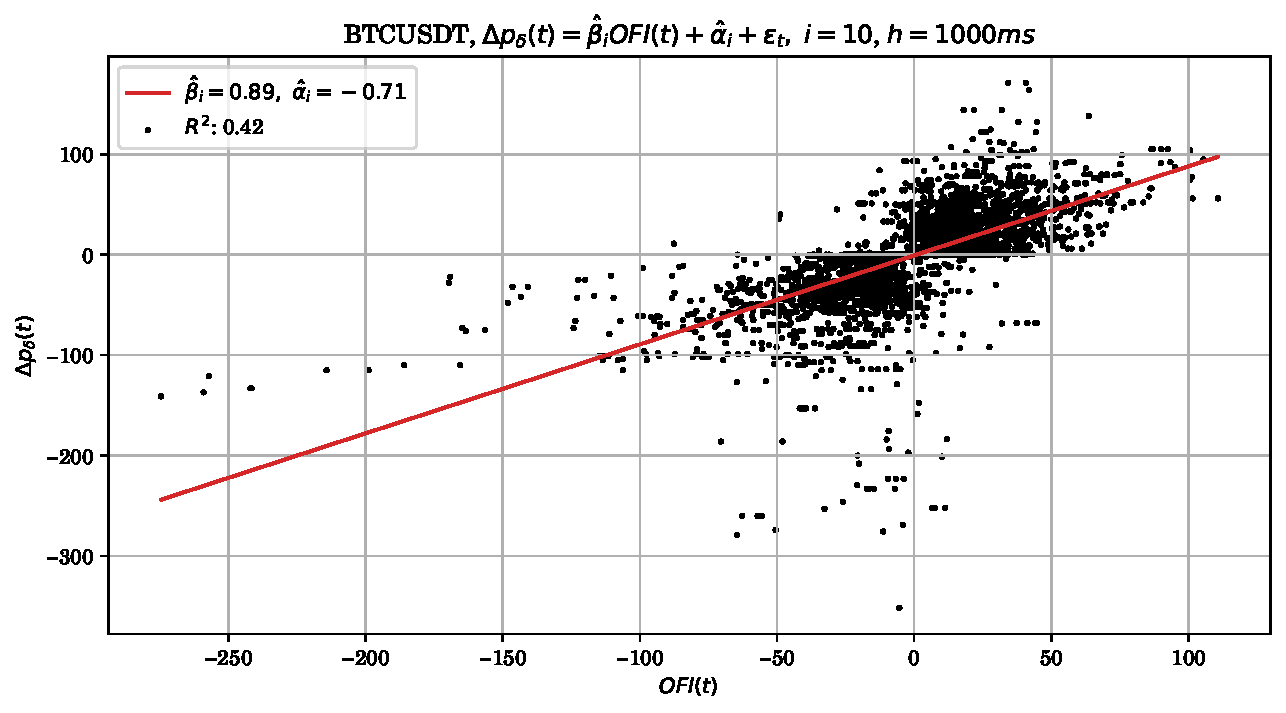
\includegraphics[width=0.8\textwidth]{./images/btcusdt_h=1000ms_contemp_OFI.pdf}
    \caption{OFI contemporaneous regression for an example half-hour window for BTCUSDT.}
\end{figure}

\clearpage




\begin{table*}
\textbf{ETHUSDT PanelOLS Results for h = 1000ms}
\begin{center}
\begin{tabular}{lclc}
\hline
\textbf{Dep. Variable:}    &         $\Delta p_{\delta}$         & \textbf{  R-squared:         }   &      0.3407      \\
\textbf{Estimator:}        &      PanelOLS      & \textbf{  R-squared (Between):}  &     -0.5821      \\
\textbf{No. Observations:} &      13612890      & \textbf{  R-squared (Within):}   &      0.3407      \\
\textbf{Date:}             &  Tue, Mar 26 2024  & \textbf{  R-squared (Overall):}  &      0.3401      \\
\textbf{Time:}             &      16:18:43      & \textbf{  Log-likelihood     }   &    -5.922e+07    \\
\textbf{Cov. Estimator:}   &     Clustered      & \textbf{                     }   &                  \\
\textbf{}                  &                    & \textbf{  F-statistic:       }   &    7.034e+06     \\
\textbf{Entities:}         &        956         & \textbf{  P-value            }   &      0.0000      \\
\textbf{Avg Obs:}          &     1.424e+04      & \textbf{  Distribution:      }   &  F(1,13611933)   \\
\textbf{Min Obs:}          &     1.058e+04      & \textbf{                     }   &                  \\
\textbf{Max Obs:}          &     1.654e+04      & \textbf{  F-statistic (robust):} &      4554.0      \\
\textbf{}                  &                    & \textbf{  P-value            }   &      0.0000      \\
\textbf{Time periods:}     &       16538        & \textbf{  Distribution:      }   &  F(1,13611933)   \\
\textbf{Avg Obs:}          &       823.13       & \textbf{                     }   &                  \\
\textbf{Min Obs:}          &       1.0000       & \textbf{                     }   &                  \\
\textbf{Max Obs:}          &       956.00       & \textbf{                     }   &                  \\
\textbf{}                  &                    & \textbf{                     }   &                  \\
\hline
\end{tabular}
\begin{tabular}{lcccccc}
             & \textbf{Parameter} & \textbf{Std. Err.} & \textbf{T-stat} & \textbf{P-value} & \textbf{Lower CI} & \textbf{Upper CI}  \\
\hline
\textbf{OFI} &       0.0891       &       0.0013       &      67.483     &      0.0000      &       0.0866      &       0.0917       \\
\hline
\end{tabular}
%\caption{PanelOLS Estimation Summary}
\end{center}
F-test for Poolability: 21.726, \\
Distribution: F(955,13611933), \\
Included effects: Entity.
\end{table*}

\begin{figure*}[htpb]
    \centering
    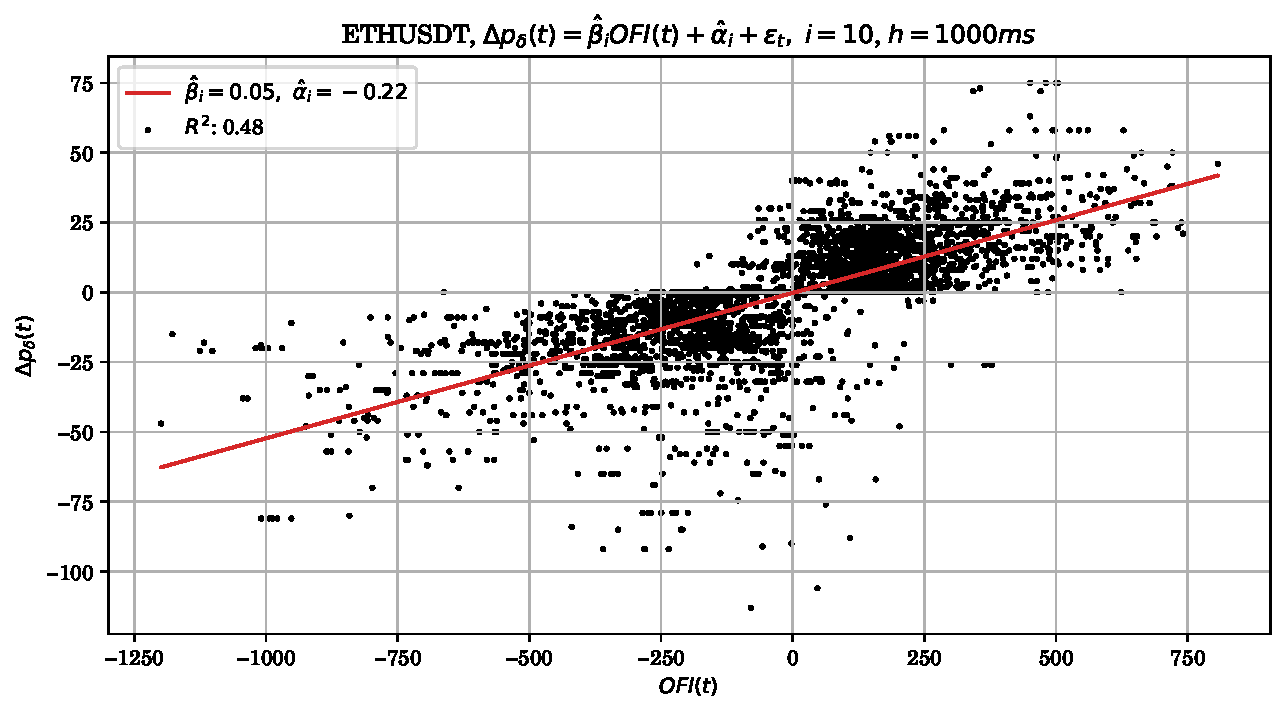
\includegraphics[width=0.8\textwidth]{./images/ethusdt_h=1000ms_contemp_OFI.pdf}
    \caption{OFI contemporaneous regression for an example half-hour window for ETHUSDT.}
\end{figure*}
\clearpage




\begin{table*}
\textbf{SOLUSDT PanelOLS Results for h = 1000ms}
\begin{center}
\begin{tabular}{lclc}
\hline
\textbf{Dep. Variable:}    &         $\Delta p_{\delta}$         & \textbf{  R-squared:         }   &      0.2828      \\
\textbf{Estimator:}        &      PanelOLS      & \textbf{  R-squared (Between):}  &     -0.3992      \\
\textbf{No. Observations:} &      13334051      & \textbf{  R-squared (Within):}   &      0.2828      \\
\textbf{Date:}             &  Tue, Mar 26 2024  & \textbf{  R-squared (Overall):}  &      0.2824      \\
\textbf{Time:}             &      16:21:12      & \textbf{  Log-likelihood     }   &    -5.176e+07    \\
\textbf{Cov. Estimator:}   &     Clustered      & \textbf{                     }   &                  \\
\textbf{}                  &                    & \textbf{  F-statistic:       }   &    5.258e+06     \\
\textbf{Entities:}         &        957         & \textbf{  P-value            }   &      0.0000      \\
\textbf{Avg Obs:}          &     1.393e+04      & \textbf{  Distribution:      }   &  F(1,13333093)   \\
\textbf{Min Obs:}          &       7478.0       & \textbf{                     }   &                  \\
\textbf{Max Obs:}          &     1.647e+04      & \textbf{  F-statistic (robust):} &      428.29      \\
\textbf{}                  &                    & \textbf{  P-value            }   &      0.0000      \\
\textbf{Time periods:}     &       16473        & \textbf{  Distribution:      }   &  F(1,13333093)   \\
\textbf{Avg Obs:}          &       809.45       & \textbf{                     }   &                  \\
\textbf{Min Obs:}          &       1.0000       & \textbf{                     }   &                  \\
\textbf{Max Obs:}          &       957.00       & \textbf{                     }   &                  \\
\textbf{}                  &                    & \textbf{                     }   &                  \\
\hline
\end{tabular}
\begin{tabular}{lcccccc}
             & \textbf{Parameter} & \textbf{Std. Err.} & \textbf{T-stat} & \textbf{P-value} & \textbf{Lower CI} & \textbf{Upper CI}  \\
\hline
\textbf{OFI} &       0.0128       &       0.0006       &      20.695     &      0.0000      &       0.0116      &       0.0140       \\
\hline
\end{tabular}
%\caption{PanelOLS Estimation Summary}
\end{center}
F-test for Poolability: 15.871, \\
Distribution: F(956,13333093), \\
Included effects: Entity.
\end{table*}

\begin{figure*}[htpb]
    \centering
    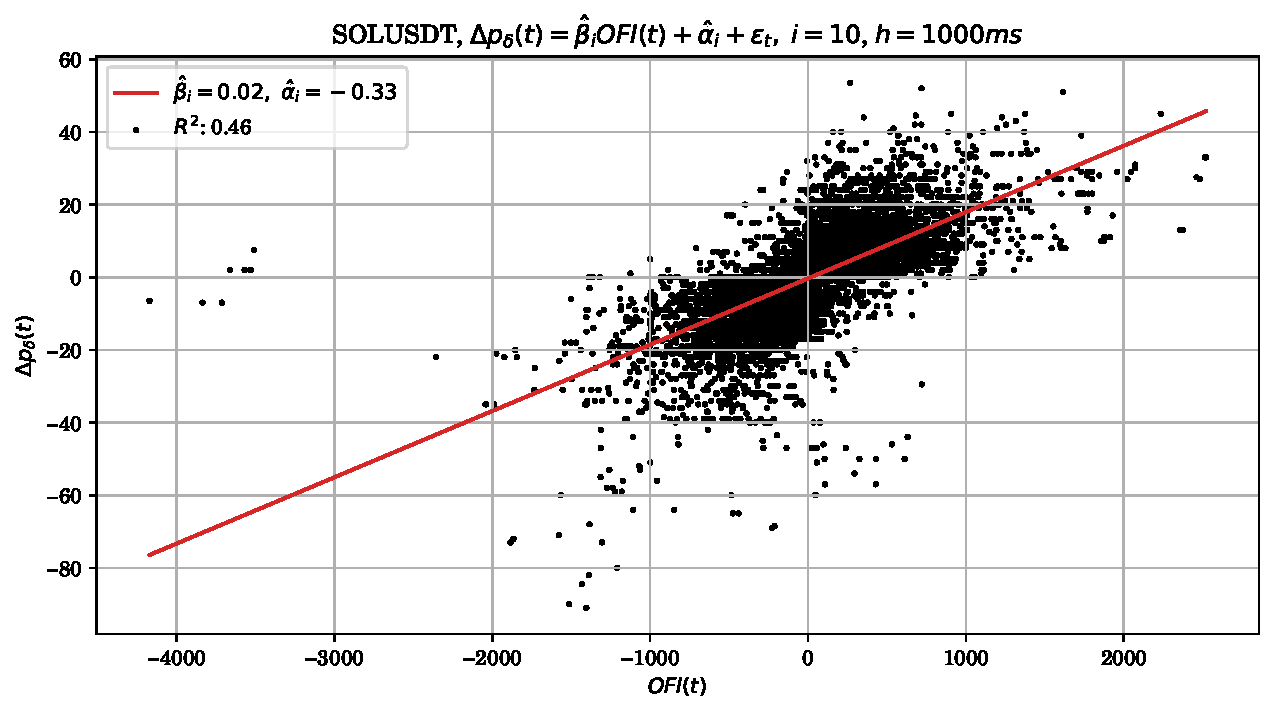
\includegraphics[width=0.8\textwidth]{./images/solusdt_h=1000ms_contemp_OFI.pdf}
    \caption{OFI contemporaneous regression for an example half-hour window for SOLUSDT.}
\end{figure*}

\clearpage




\begin{table*}
\textbf{MATICUSDT PanelOLS Results for h = 1000ms}
\begin{center}
\begin{tabular}{lclc}
\hline
\textbf{Dep. Variable:}    &         $\Delta p_{\delta}$         & \textbf{  R-squared:         }   &      0.4133      \\
\textbf{Estimator:}        &      PanelOLS      & \textbf{  R-squared (Between):}  &     -0.0188      \\
\textbf{No. Observations:} &      11294487      & \textbf{  R-squared (Within):}   &      0.4133      \\
\textbf{Date:}             &  Tue, Mar 26 2024  & \textbf{  R-squared (Overall):}  &      0.4130      \\
\textbf{Time:}             &      16:23:26      & \textbf{  Log-likelihood     }   &    -1.58e+07     \\
\textbf{Cov. Estimator:}   &     Clustered      & \textbf{                     }   &                  \\
\textbf{}                  &                    & \textbf{  F-statistic:       }   &    7.955e+06     \\
\textbf{Entities:}         &        956         & \textbf{  P-value            }   &      0.0000      \\
\textbf{Avg Obs:}          &     1.181e+04      & \textbf{  Distribution:      }   &  F(1,11293530)   \\
\textbf{Min Obs:}          &       5754.0       & \textbf{                     }   &                  \\
\textbf{Max Obs:}          &     1.639e+04      & \textbf{  F-statistic (robust):} &      2882.6      \\
\textbf{}                  &                    & \textbf{  P-value            }   &      0.0000      \\
\textbf{Time periods:}     &       16388        & \textbf{  Distribution:      }   &  F(1,11293530)   \\
\textbf{Avg Obs:}          &       689.19       & \textbf{                     }   &                  \\
\textbf{Min Obs:}          &       1.0000       & \textbf{                     }   &                  \\
\textbf{Max Obs:}          &       956.00       & \textbf{                     }   &                  \\
\textbf{}                  &                    & \textbf{                     }   &                  \\
\hline
\end{tabular}
\begin{tabular}{lcccccc}
             & \textbf{Parameter} & \textbf{Std. Err.} & \textbf{T-stat} & \textbf{P-value} & \textbf{Lower CI} & \textbf{Upper CI}  \\
\hline
\textbf{OFI} &     3.108e-05      &     5.789e-07      &      53.690     &      0.0000      &     2.995e-05     &     3.222e-05      \\
\hline
\end{tabular}
%\caption{PanelOLS Estimation Summary}
\end{center}
F-test for Poolability: 15.992, \\
Distribution: F(955,11293530), \\
Included effects: Entity.
\end{table*}

\begin{figure*}[htpb]
    \centering
    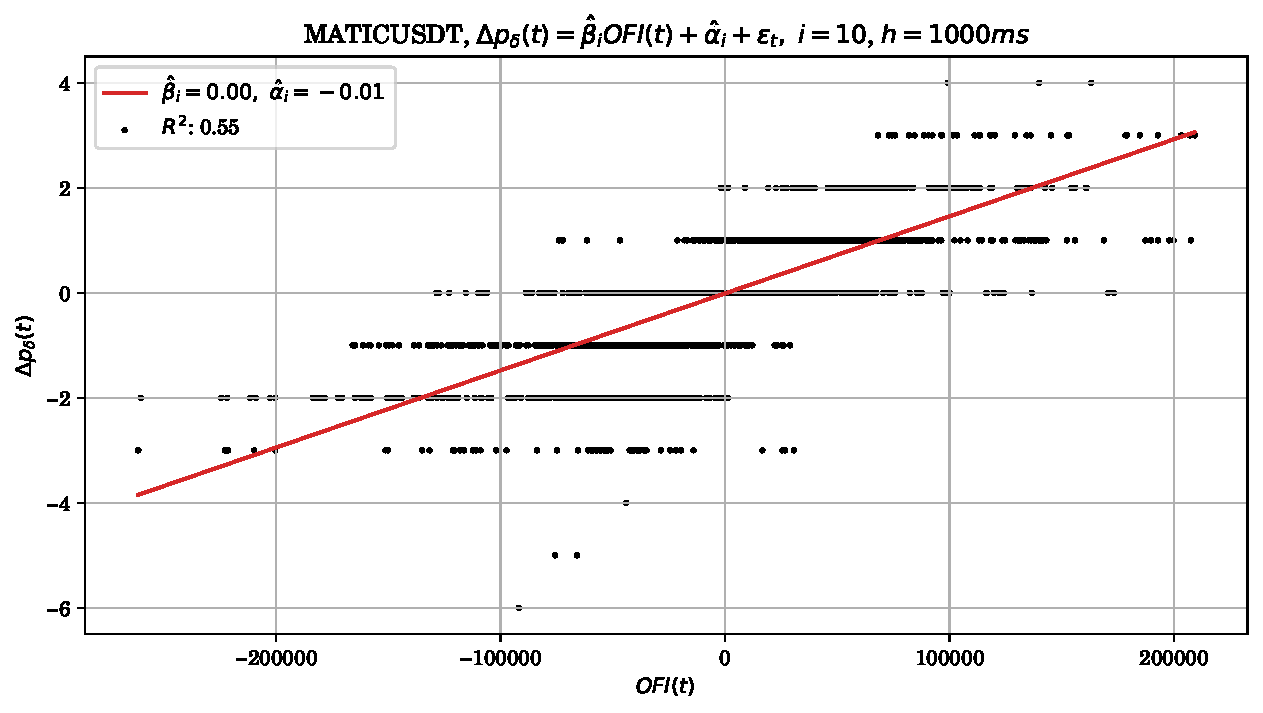
\includegraphics[width=0.8\textwidth]{./images/maticusdt_h=1000ms_contemp_OFI.pdf}
    \caption{OFI contemporaneous regression for an example half-hour window for MATICUSDT.}
    \label{fig:contemp_OFI_maticusdt}
\end{figure*}


\chapter{Websocket Data Summary Statistics}
\hrule
\vspace{2em}
We present the summary statistics for the entire dataset for each trading pair here.
For each trading pair we have approximately 13 million observations ranging from 2024-02-05 13:07:53.664 to 2024-02-25 11:18:50.866.

\begin{table}[ht] 
\resizebox{0.99\textwidth}{!}{
\begin{tabular}{lrrrrrrrrrr}
\toprule
 & ask\_qty\_1 & ask\_qty\_2 & ask\_qty\_3 & ask\_qty\_4 & ask\_qty\_5 & ask\_qty\_6 & ask\_qty\_7 & ask\_qty\_8 & ask\_qty\_9 & ask\_qty\_10 \\
\midrule
count & 12891081.00 & 12891081.00 & 12891081.00 & 12891081.00 & 12891081.00 & 12891081.00 & 12891081.00 & 12891081.00 & 12891081.00 & 12891081.00 \\
mean & 6.20 & 0.34 & 0.31 & 0.33 & 0.34 & 0.33 & 0.32 & 0.32 & 0.32 & 0.31 \\
std & 8.37 & 2.04 & 1.57 & 1.81 & 2.24 & 2.23 & 2.38 & 2.25 & 2.61 & 2.38 \\
min & 0.00 & 0.00 & 0.00 & 0.00 & 0.00 & 0.00 & 0.00 & 0.00 & 0.00 & 0.00 \\
25\% & 1.93 & 0.00 & 0.01 & 0.01 & 0.01 & 0.01 & 0.01 & 0.01 & 0.01 & 0.01 \\
50\% & 4.66 & 0.01 & 0.05 & 0.05 & 0.05 & 0.05 & 0.05 & 0.05 & 0.05 & 0.05 \\
75\% & 8.41 & 0.18 & 0.21 & 0.24 & 0.24 & 0.24 & 0.24 & 0.24 & 0.24 & 0.24 \\
max & 859.16 & 559.55 & 802.35 & 796.21 & 499.30 & 989.40 & 558.80 & 584.51 & 680.40 & 584.51 \\
\bottomrule
\end{tabular}
}

\resizebox{0.99\textwidth}{!}{
\begin{tabular}{lrrrrrrrrrr}
\toprule
 & bid\_qty\_1 & bid\_qty\_2 & bid\_qty\_3 & bid\_qty\_4 & bid\_qty\_5 & bid\_qty\_6 & bid\_qty\_7 & bid\_qty\_8 & bid\_qty\_9 & bid\_qty\_10 \\
\midrule
count & 12891081.00 & 12891081.00 & 12891081.00 & 12891081.00 & 12891081.00 & 12891081.00 & 12891081.00 & 12891081.00 & 12891081.00 & 12891081.00 \\
mean & 6.23 & 0.38 & 0.31 & 0.34 & 0.34 & 0.32 & 0.32 & 0.31 & 0.31 & 0.30 \\
std & 10.27 & 2.63 & 1.77 & 2.66 & 2.53 & 2.01 & 2.25 & 2.21 & 2.37 & 2.19 \\
min & 0.00 & 0.00 & 0.00 & 0.00 & 0.00 & 0.00 & 0.00 & 0.00 & 0.00 & 0.00 \\
25\% & 1.98 & 0.00 & 0.01 & 0.01 & 0.01 & 0.01 & 0.01 & 0.01 & 0.01 & 0.01 \\
50\% & 4.63 & 0.02 & 0.05 & 0.05 & 0.05 & 0.05 & 0.05 & 0.05 & 0.05 & 0.05 \\
75\% & 8.40 & 0.21 & 0.22 & 0.24 & 0.24 & 0.24 & 0.23 & 0.23 & 0.23 & 0.23 \\
max & 1008.05 & 861.61 & 777.20 & 781.40 & 781.40 & 781.40 & 997.10 & 997.10 & 997.41 & 767.82 \\
\bottomrule
\end{tabular}
}

\resizebox{0.99\textwidth}{!}{
\begin{tabular}{lrrrrrrrrrr}
\toprule
 & ask\_price\_1 & ask\_price\_2 & ask\_price\_3 & ask\_price\_4 & ask\_price\_5 & ask\_price\_6 & ask\_price\_7 & ask\_price\_8 & ask\_price\_9 & ask\_price\_10 \\
\midrule
count & 12891081.00 & 12891081.00 & 12891081.00 & 12891081.00 & 12891081.00 & 12891081.00 & 12891081.00 & 12891081.00 & 12891081.00 & 12891081.00 \\
mean & 49385.06 & 49385.19 & 49385.45 & 49385.68 & 49385.90 & 49386.10 & 49386.30 & 49386.48 & 49386.66 & 49386.83 \\
std & 3107.13 & 3107.13 & 3107.15 & 3107.16 & 3107.17 & 3107.18 & 3107.19 & 3107.19 & 3107.20 & 3107.21 \\
min & 42311.30 & 42311.40 & 42312.00 & 42312.10 & 42312.60 & 42313.10 & 42313.40 & 42313.60 & 42313.80 & 42313.90 \\
25\% & 47454.30 & 47454.40 & 47454.60 & 47454.90 & 47455.20 & 47455.50 & 47455.70 & 47455.90 & 47456.00 & 47456.20 \\
50\% & 51086.00 & 51086.20 & 51086.30 & 51086.50 & 51086.80 & 51087.00 & 51087.20 & 51087.40 & 51087.60 & 51087.80 \\
75\% & 51790.00 & 51790.10 & 51790.40 & 51790.60 & 51790.80 & 51791.00 & 51791.20 & 51791.50 & 51791.80 & 51791.90 \\
max & 53087.70 & 53087.90 & 53088.70 & 53089.80 & 53090.00 & 53090.20 & 53090.50 & 53090.80 & 53090.90 & 53091.00 \\
\bottomrule
\end{tabular}
}

\resizebox{0.99\textwidth}{!}{
\begin{tabular}{lrrrrrrrrrr}
\toprule
 & bid\_price\_1 & bid\_price\_2 & bid\_price\_3 & bid\_price\_4 & bid\_price\_5 & bid\_price\_6 & bid\_price\_7 & bid\_price\_8 & bid\_price\_9 & bid\_price\_10 \\
\midrule
count & 12891081.00 & 12891081.00 & 12891081.00 & 12891081.00 & 12891081.00 & 12891081.00 & 12891081.00 & 12891081.00 & 12891081.00 & 12891081.00 \\
mean & 49384.96 & 49384.83 & 49384.57 & 49384.34 & 49384.12 & 49383.92 & 49383.72 & 49383.54 & 49383.36 & 49383.19 \\
std & 3107.13 & 3107.13 & 3107.12 & 3107.10 & 3107.09 & 3107.08 & 3107.08 & 3107.07 & 3107.06 & 3107.06 \\
min & 42311.20 & 42311.10 & 42311.00 & 42310.90 & 42310.80 & 42310.70 & 42310.60 & 42310.50 & 42310.40 & 42310.30 \\
25\% & 47454.20 & 47454.10 & 47453.80 & 47453.60 & 47453.40 & 47453.20 & 47453.00 & 47452.90 & 47452.60 & 47452.50 \\
50\% & 51085.90 & 51085.70 & 51085.40 & 51085.20 & 51085.00 & 51084.90 & 51084.70 & 51084.50 & 51084.40 & 51084.20 \\
75\% & 51789.90 & 51789.80 & 51789.50 & 51789.30 & 51789.00 & 51788.80 & 51788.50 & 51788.40 & 51788.20 & 51788.00 \\
max & 53087.30 & 53086.80 & 53086.70 & 53085.90 & 53084.30 & 53081.90 & 53080.00 & 53079.00 & 53078.70 & 53078.10 \\
\bottomrule
\end{tabular}
}

\caption{Summary statistics for BTCUSDT websocket data.}
\end{table}


\begin{table}[ht] 
\resizebox{0.99\textwidth}{!}{
\begin{tabular}{lrrrrrrrrrr}
\toprule
 & ask\_qty\_1 & ask\_qty\_2 & ask\_qty\_3 & ask\_qty\_4 & ask\_qty\_5 & ask\_qty\_6 & ask\_qty\_7 & ask\_qty\_8 & ask\_qty\_9 & ask\_qty\_10 \\
\midrule
count & 13612891.00 & 13612891.00 & 13612891.00 & 13612891.00 & 13612891.00 & 13612891.00 & 13612891.00 & 13612891.00 & 13612891.00 & 13612891.00 \\
mean & 55.23 & 3.62 & 3.09 & 3.56 & 3.63 & 4.02 & 4.26 & 4.50 & 4.79 & 4.97 \\
std & 99.00 & 32.41 & 26.30 & 26.81 & 25.79 & 30.65 & 28.90 & 25.88 & 28.91 & 26.91 \\
min & 0.00 & 0.00 & 0.00 & 0.00 & 0.00 & 0.00 & 0.00 & 0.00 & 0.00 & 0.00 \\
25\% & 14.98 & 0.01 & 0.07 & 0.07 & 0.08 & 0.08 & 0.10 & 0.13 & 0.16 & 0.18 \\
50\% & 35.91 & 0.15 & 0.43 & 0.50 & 0.57 & 0.69 & 0.95 & 1.08 & 1.23 & 1.43 \\
75\% & 71.94 & 2.15 & 2.92 & 3.06 & 3.29 & 3.58 & 3.90 & 4.15 & 4.53 & 5.00 \\
max & 7612.08 & 7357.27 & 5443.50 & 5926.07 & 7315.07 & 5873.18 & 7974.45 & 5696.58 & 6124.07 & 6123.37 \\
\bottomrule
\end{tabular}
}

\resizebox{0.99\textwidth}{!}{
\begin{tabular}{lrrrrrrrrrr}
\toprule
 & bid\_qty\_1 & bid\_qty\_2 & bid\_qty\_3 & bid\_qty\_4 & bid\_qty\_5 & bid\_qty\_6 & bid\_qty\_7 & bid\_qty\_8 & bid\_qty\_9 & bid\_qty\_10 \\
\midrule
count & 13612891.00 & 13612891.00 & 13612891.00 & 13612891.00 & 13612891.00 & 13612891.00 & 13612891.00 & 13612891.00 & 13612891.00 & 13612891.00 \\
mean & 53.26 & 3.63 & 3.10 & 3.53 & 3.67 & 3.82 & 4.29 & 4.38 & 4.66 & 4.85 \\
std & 89.38 & 31.08 & 21.56 & 27.54 & 25.38 & 25.80 & 30.64 & 25.90 & 25.48 & 22.62 \\
min & 0.00 & 0.00 & 0.00 & 0.00 & 0.00 & 0.00 & 0.00 & 0.00 & 0.00 & 0.00 \\
25\% & 14.85 & 0.01 & 0.08 & 0.08 & 0.08 & 0.08 & 0.11 & 0.14 & 0.17 & 0.20 \\
50\% & 35.25 & 0.20 & 0.44 & 0.52 & 0.60 & 0.71 & 1.00 & 1.12 & 1.28 & 1.48 \\
75\% & 71.20 & 2.40 & 2.97 & 3.05 & 3.28 & 3.55 & 3.86 & 4.10 & 4.48 & 4.98 \\
max & 10228.23 & 10221.75 & 10221.74 & 10221.74 & 9607.48 & 1.02 & 9829.58 & 10224.01 & 7143.02 & 9817.49 \\
\bottomrule
\end{tabular}
}

\resizebox{0.99\textwidth}{!}{
\begin{tabular}{lrrrrrrrrrr}
\toprule
 & ask\_price\_1 & ask\_price\_2 & ask\_price\_3 & ask\_price\_4 & ask\_price\_5 & ask\_price\_6 & ask\_price\_7 & ask\_price\_8 & ask\_price\_9 & ask\_price\_10 \\
\midrule
count & 13612891.00 & 13612891.00 & 13612891.00 & 13612891.00 & 13612891.00 & 13612891.00 & 13612891.00 & 13612891.00 & 13612891.00 & 13612891.00 \\
mean & 2704.80 & 2704.81 & 2704.83 & 2704.85 & 2704.87 & 2704.88 & 2704.90 & 2704.91 & 2704.93 & 2704.94 \\
std & 223.88 & 223.88 & 223.88 & 223.88 & 223.89 & 223.89 & 223.89 & 223.89 & 223.89 & 223.89 \\
min & 2282.36 & 2282.38 & 2282.40 & 2282.41 & 2282.42 & 2282.44 & 2282.46 & 2282.47 & 2282.48 & 2282.49 \\
25\% & 2494.37 & 2494.38 & 2494.40 & 2494.41 & 2494.43 & 2494.44 & 2494.46 & 2494.47 & 2494.48 & 2494.50 \\
50\% & 2776.17 & 2776.18 & 2776.20 & 2776.21 & 2776.23 & 2776.25 & 2776.26 & 2776.28 & 2776.29 & 2776.31 \\
75\% & 2920.21 & 2920.23 & 2920.24 & 2920.26 & 2920.28 & 2920.30 & 2920.32 & 2920.33 & 2920.35 & 2920.36 \\
max & 3053.11 & 3053.12 & 3053.32 & 3053.51 & 3053.54 & 3053.59 & 3053.69 & 3053.70 & 3053.71 & 3053.72 \\
\bottomrule
\end{tabular}
}

\resizebox{0.99\textwidth}{!}{
\begin{tabular}{lrrrrrrrrrr}
\toprule
 & bid\_price\_1 & bid\_price\_2 & bid\_price\_3 & bid\_price\_4 & bid\_price\_5 & bid\_price\_6 & bid\_price\_7 & bid\_price\_8 & bid\_price\_9 & bid\_price\_10 \\
\midrule
count & 13612891.00 & 13612891.00 & 13612891.00 & 13612891.00 & 13612891.00 & 13612891.00 & 13612891.00 & 13612891.00 & 13612891.00 & 13612891.00 \\
mean & 2704.79 & 2704.78 & 2704.76 & 2704.74 & 2704.72 & 2704.71 & 2704.69 & 2704.67 & 2704.66 & 2704.65 \\
std & 223.88 & 223.88 & 223.88 & 223.88 & 223.87 & 223.87 & 223.87 & 223.87 & 223.87 & 223.87 \\
min & 2282.35 & 2282.32 & 2282.31 & 2282.28 & 2282.27 & 2282.23 & 2282.21 & 2282.20 & 2282.17 & 2282.16 \\
25\% & 2494.36 & 2494.35 & 2494.33 & 2494.32 & 2494.30 & 2494.28 & 2494.27 & 2494.26 & 2494.24 & 2494.23 \\
50\% & 2776.16 & 2776.15 & 2776.12 & 2776.10 & 2776.08 & 2776.06 & 2776.05 & 2776.03 & 2776.02 & 2776.00 \\
75\% & 2920.20 & 2920.19 & 2920.17 & 2920.15 & 2920.13 & 2920.12 & 2920.10 & 2920.08 & 2920.07 & 2920.05 \\
max & 3053.10 & 3053.09 & 3053.07 & 3053.06 & 3053.03 & 3053.02 & 3052.99 & 3052.96 & 3052.95 & 3052.89 \\
\bottomrule
\end{tabular}
}

\resizebox{0.99\textwidth}{!}{
}\caption{Summary statistics for ETHUSDT websocket data.}
\end{table}
\begin{table}[ht] 
\resizebox{0.99\textwidth}{!}{
\begin{tabular}{lrrrrrrrrrr}
\toprule
 & ask\_qty\_1 & ask\_qty\_2 & ask\_qty\_3 & ask\_qty\_4 & ask\_qty\_5 & ask\_qty\_6 & ask\_qty\_7 & ask\_qty\_8 & ask\_qty\_9 & ask\_qty\_10 \\
\midrule
count & 11294488.00 & 11294488.00 & 11294488.00 & 11294488.00 & 11294488.00 & 11294488.00 & 11294488.00 & 11294488.00 & 11294488.00 & 11294488.00 \\
mean & 12716.18 & 23685.36 & 38829.90 & 49438.51 & 58123.57 & 62507.59 & 60930.95 & 55367.95 & 49777.05 & 45230.33 \\
std & 19985.48 & 21545.45 & 33115.61 & 33501.64 & 36397.22 & 36074.49 & 34204.86 & 31431.88 & 29423.23 & 27729.75 \\
min & 1.00 & 1.00 & 2.00 & 5.00 & 5.00 & 5.00 & 5.00 & 5.00 & 5.00 & 5.00 \\
25\% & 5269.00 & 13057.00 & 18610.00 & 27384.00 & 33447.00 & 38708.00 & 39230.00 & 36148.00 & 31811.00 & 28155.00 \\
50\% & 10097.00 & 19536.00 & 29812.00 & 42883.00 & 52081.00 & 57505.00 & 56367.00 & 51253.00 & 45577.00 & 41255.00 \\
75\% & 16399.00 & 28774.00 & 50104.00 & 64126.00 & 75982.00 & 80202.00 & 76991.00 & 69533.00 & 62500.00 & 57491.00 \\
max & 2921095.00 & 2431682.00 & 2917345.00 & 2436953.00 & 2436953.00 & 2150536.00 & 2150151.00 & 2172650.00 & 2166177.00 & 2110610.00 \\
\bottomrule
\end{tabular}
}

\resizebox{0.99\textwidth}{!}{
\begin{tabular}{lrrrrrrrrrr}
\toprule
 & bid\_qty\_1 & bid\_qty\_2 & bid\_qty\_3 & bid\_qty\_4 & bid\_qty\_5 & bid\_qty\_6 & bid\_qty\_7 & bid\_qty\_8 & bid\_qty\_9 & bid\_qty\_10 \\
\midrule
count & 11294488.00 & 11294488.00 & 11294488.00 & 11294488.00 & 11294488.00 & 11294488.00 & 11294488.00 & 11294488.00 & 11294488.00 & 11294488.00 \\
mean & 12779.39 & 23928.98 & 38887.18 & 46815.71 & 54853.76 & 59332.21 & 58452.96 & 54253.30 & 49710.25 & 45841.90 \\
std & 20186.24 & 30727.91 & 43285.03 & 40321.36 & 44909.71 & 43983.18 & 41601.12 & 42093.02 & 39812.07 & 38648.16 \\
min & 1.00 & 1.00 & 1.00 & 1.00 & 1.00 & 6.00 & 5.00 & 6.00 & 6.00 & 6.00 \\
25\% & 5178.00 & 13061.00 & 17648.00 & 24198.00 & 28938.00 & 33737.00 & 35554.00 & 34653.00 & 31671.00 & 28502.00 \\
50\% & 10013.00 & 19524.00 & 28130.00 & 39084.00 & 46815.00 & 52633.00 & 52927.00 & 49867.00 & 45679.00 & 41671.00 \\
75\% & 16379.00 & 28632.00 & 49179.00 & 60990.00 & 72526.00 & 77182.00 & 74448.00 & 67999.00 & 62337.00 & 57838.00 \\
max & 3795122.00 & 3817190.00 & 3817875.00 & 3827721.00 & 3849124.00 & 3850149.00 & 3860481.00 & 3881703.00 & 3890275.00 & 3885535.00 \\
\bottomrule
\end{tabular}
}

\resizebox{0.99\textwidth}{!}{
\begin{tabular}{lrrrrrrrrrr}
\toprule
 & ask\_price\_1 & ask\_price\_2 & ask\_price\_3 & ask\_price\_4 & ask\_price\_5 & ask\_price\_6 & ask\_price\_7 & ask\_price\_8 & ask\_price\_9 & ask\_price\_10 \\
\midrule
count & 11294488.00 & 11294488.00 & 11294488.00 & 11294488.00 & 11294488.00 & 11294488.00 & 11294488.00 & 11294488.00 & 11294488.00 & 11294488.00 \\
mean & 0.91 & 0.91 & 0.91 & 0.91 & 0.91 & 0.91 & 0.91 & 0.91 & 0.91 & 0.91 \\
std & 0.07 & 0.07 & 0.07 & 0.07 & 0.07 & 0.07 & 0.07 & 0.07 & 0.07 & 0.07 \\
min & 0.77 & 0.77 & 0.77 & 0.77 & 0.77 & 0.77 & 0.77 & 0.77 & 0.77 & 0.77 \\
25\% & 0.85 & 0.85 & 0.85 & 0.85 & 0.85 & 0.85 & 0.85 & 0.85 & 0.85 & 0.85 \\
50\% & 0.90 & 0.90 & 0.90 & 0.90 & 0.90 & 0.90 & 0.90 & 0.90 & 0.90 & 0.90 \\
75\% & 0.98 & 0.98 & 0.98 & 0.98 & 0.98 & 0.98 & 0.98 & 0.98 & 0.98 & 0.98 \\
max & 1.07 & 1.07 & 1.07 & 1.07 & 1.07 & 1.07 & 1.07 & 1.07 & 1.07 & 1.07 \\
\bottomrule
\end{tabular}
}

\resizebox{0.99\textwidth}{!}{
\begin{tabular}{lrrrrrrrrrr}
\toprule
 & bid\_price\_1 & bid\_price\_2 & bid\_price\_3 & bid\_price\_4 & bid\_price\_5 & bid\_price\_6 & bid\_price\_7 & bid\_price\_8 & bid\_price\_9 & bid\_price\_10 \\
\midrule
count & 11294488.00 & 11294488.00 & 11294488.00 & 11294488.00 & 11294488.00 & 11294488.00 & 11294488.00 & 11294488.00 & 11294488.00 & 11294488.00 \\
mean & 0.91 & 0.91 & 0.91 & 0.91 & 0.91 & 0.91 & 0.91 & 0.91 & 0.90 & 0.90 \\
std & 0.07 & 0.07 & 0.07 & 0.07 & 0.07 & 0.07 & 0.07 & 0.07 & 0.07 & 0.07 \\
min & 0.77 & 0.77 & 0.77 & 0.77 & 0.77 & 0.77 & 0.77 & 0.77 & 0.77 & 0.77 \\
25\% & 0.85 & 0.85 & 0.85 & 0.85 & 0.85 & 0.84 & 0.84 & 0.84 & 0.84 & 0.84 \\
50\% & 0.90 & 0.90 & 0.90 & 0.90 & 0.90 & 0.90 & 0.90 & 0.90 & 0.90 & 0.90 \\
75\% & 0.98 & 0.97 & 0.97 & 0.97 & 0.97 & 0.97 & 0.97 & 0.97 & 0.97 & 0.97 \\
max & 1.06 & 1.06 & 1.06 & 1.06 & 1.06 & 1.06 & 1.06 & 1.06 & 1.06 & 1.06 \\
\bottomrule
\end{tabular}
}

\resizebox{0.99\textwidth}{!}{
}\caption{Summary statistics for MATICUSDT websocket data.}
\end{table}
\begin{table}[ht] 
\resizebox{0.99\textwidth}{!}{
\begin{tabular}{lrrrrrrrrrr}
\toprule
 & ask\_qty\_1 & ask\_qty\_2 & ask\_qty\_3 & ask\_qty\_4 & ask\_qty\_5 & ask\_qty\_6 & ask\_qty\_7 & ask\_qty\_8 & ask\_qty\_9 & ask\_qty\_10 \\
\midrule
count & 13334052.00 & 13334052.00 & 13334052.00 & 13334052.00 & 13334052.00 & 13334052.00 & 13334052.00 & 13334052.00 & 13334052.00 & 13334052.00 \\
mean & 145.89 & 39.46 & 39.46 & 42.48 & 45.36 & 49.41 & 49.24 & 51.38 & 53.52 & 53.52 \\
std & 612.39 & 329.36 & 307.82 & 313.65 & 338.84 & 343.93 & 340.86 & 351.44 & 404.63 & 374.13 \\
min & 1.00 & 1.00 & 1.00 & 1.00 & 1.00 & 1.00 & 1.00 & 1.00 & 1.00 & 1.00 \\
25\% & 30.00 & 3.00 & 5.00 & 6.00 & 7.00 & 8.00 & 8.00 & 9.00 & 10.00 & 10.00 \\
50\% & 82.00 & 13.00 & 17.00 & 20.00 & 20.00 & 22.00 & 23.00 & 25.00 & 26.00 & 26.00 \\
75\% & 165.00 & 43.00 & 44.00 & 47.00 & 48.00 & 53.00 & 53.00 & 56.00 & 57.00 & 57.00 \\
max & 100015.00 & 96598.00 & 92722.00 & 96614.00 & 96654.00 & 96655.00 & 96615.00 & 66776.00 & 96596.00 & 96654.00 \\
\bottomrule
\end{tabular}
}

\resizebox{0.99\textwidth}{!}{
\begin{tabular}{lrrrrrrrrrr}
\toprule
 & bid\_qty\_1 & bid\_qty\_2 & bid\_qty\_3 & bid\_qty\_4 & bid\_qty\_5 & bid\_qty\_6 & bid\_qty\_7 & bid\_qty\_8 & bid\_qty\_9 & bid\_qty\_10 \\
\midrule
count & 13334052.00 & 13334052.00 & 13334052.00 & 13334052.00 & 13334052.00 & 13334052.00 & 13334052.00 & 13334052.00 & 13334052.00 & 13334052.00 \\
mean & 149.28 & 41.87 & 42.54 & 43.52 & 46.18 & 50.08 & 50.02 & 52.05 & 53.16 & 54.65 \\
std & 863.95 & 560.08 & 587.61 & 506.86 & 534.82 & 561.51 & 571.15 & 567.41 & 563.31 & 632.98 \\
min & 1.00 & 1.00 & 1.00 & 1.00 & 1.00 & 1.00 & 1.00 & 1.00 & 1.00 & 1.00 \\
25\% & 28.00 & 3.00 & 5.00 & 6.00 & 6.00 & 7.00 & 8.00 & 9.00 & 9.00 & 10.00 \\
50\% & 80.00 & 13.00 & 17.00 & 19.00 & 20.00 & 21.00 & 22.00 & 24.00 & 25.00 & 26.00 \\
75\% & 163.00 & 43.00 & 44.00 & 47.00 & 47.00 & 51.00 & 51.00 & 54.00 & 55.00 & 55.00 \\
max & 119226.00 & 119696.00 & 112113.00 & 100918.00 & 102320.00 & 100934.00 & 100916.00 & 100916.00 & 100916.00 & 100913.00 \\
\bottomrule
\end{tabular}
}

\resizebox{0.99\textwidth}{!}{
\begin{tabular}{lrrrrrrrrrr}
\toprule
 & ask\_price\_1 & ask\_price\_2 & ask\_price\_3 & ask\_price\_4 & ask\_price\_5 & ask\_price\_6 & ask\_price\_7 & ask\_price\_8 & ask\_price\_9 & ask\_price\_10 \\
\midrule
count & 13334052.00 & 13334052.00 & 13334052.00 & 13334052.00 & 13334052.00 & 13334052.00 & 13334052.00 & 13334052.00 & 13334052.00 & 13334052.00 \\
mean & 106.70 & 106.70 & 106.70 & 106.70 & 106.71 & 106.71 & 106.71 & 106.71 & 106.71 & 106.71 \\
std & 5.83 & 5.83 & 5.83 & 5.83 & 5.83 & 5.83 & 5.83 & 5.83 & 5.83 & 5.83 \\
min & 93.13 & 93.13 & 93.14 & 93.14 & 93.14 & 93.14 & 93.14 & 93.14 & 93.14 & 93.14 \\
25\% & 102.61 & 102.61 & 102.61 & 102.61 & 102.61 & 102.62 & 102.62 & 102.62 & 102.62 & 102.62 \\
50\% & 107.52 & 107.52 & 107.53 & 107.53 & 107.53 & 107.53 & 107.53 & 107.53 & 107.53 & 107.54 \\
75\% & 111.36 & 111.37 & 111.37 & 111.37 & 111.37 & 111.37 & 111.37 & 111.37 & 111.38 & 111.38 \\
max & 118.83 & 118.83 & 118.83 & 118.83 & 118.84 & 118.84 & 118.84 & 118.84 & 118.84 & 118.84 \\
\bottomrule
\end{tabular}
}

\resizebox{0.99\textwidth}{!}{
\begin{tabular}{lrrrrrrrrrr}
\toprule
 & bid\_price\_1 & bid\_price\_2 & bid\_price\_3 & bid\_price\_4 & bid\_price\_5 & bid\_price\_6 & bid\_price\_7 & bid\_price\_8 & bid\_price\_9 & bid\_price\_10 \\
\midrule
count & 13334052.00 & 13334052.00 & 13334052.00 & 13334052.00 & 13334052.00 & 13334052.00 & 13334052.00 & 13334052.00 & 13334052.00 & 13334052.00 \\
mean & 106.70 & 106.70 & 106.70 & 106.69 & 106.69 & 106.69 & 106.69 & 106.69 & 106.69 & 106.69 \\
std & 5.83 & 5.83 & 5.83 & 5.83 & 5.83 & 5.83 & 5.83 & 5.83 & 5.83 & 5.83 \\
min & 93.13 & 93.13 & 93.13 & 93.13 & 93.13 & 93.12 & 93.12 & 93.12 & 93.12 & 93.12 \\
25\% & 102.61 & 102.61 & 102.60 & 102.60 & 102.60 & 102.60 & 102.60 & 102.60 & 102.60 & 102.60 \\
50\% & 107.52 & 107.52 & 107.52 & 107.52 & 107.52 & 107.52 & 107.51 & 107.51 & 107.51 & 107.51 \\
75\% & 111.36 & 111.36 & 111.36 & 111.36 & 111.36 & 111.36 & 111.36 & 111.36 & 111.36 & 111.35 \\
max & 118.83 & 118.82 & 118.82 & 118.82 & 118.82 & 118.82 & 118.82 & 118.82 & 118.82 & 118.82 \\
\bottomrule
\end{tabular}
}

\caption{Summary statistics for SOLUSDT websocket data.}
\end{table}


\chapter{Alternative Data Source}
\hrule
\vspace{40pt}

\section{Introduction}

Initially we were not using the Websocket endpoint to gather our data.
Instead we used the Binance historical tick-level orderbook API endpoint.
This returns compressed L2 representations of the orderbook going back multiple years and
for all available trading pairs.
This proved an interesting challenge to parse, so we present our journey here.
This is a cautionary tale, since in the end, we were unable to use this data, so
this chapter also serves as a warning for anyone looking to use this data for a similar application.

\textbf{TL;DR}: This data source has a large amount of missing data.

The data is organized into compressed directories, one for each day. In each directory
there is a snapshot file and an updates file. The snapshot file contains all levels
of the orderbook at the start of the day. See Table \ref{table:snap} \footnote{Originally the raw data was using "b" for bids and "a" for asks in the side column, but we encode bids with $1$s and asks with $0$s so that our data is entirely numerical.}
for an example of a snapshot DataFrame.

\begin{table}[H]
    \centering
    \resizebox{\textwidth}{!}{
        \begin{tabular}{ccccccc}
            \toprule
            Row & timestamp & first\_update\_id & last\_update\_id & side & price & qty \\
            \midrule
            1 & 1689033589005 & 3046269468672 & 3046269468672 & 0 & 30395.5 & 5.174 \\
            2 & 1689033589005 & 3046269468672 & 3046269468672 & 0 & 30395.6 & 0.002 \\
            3 & 1689033589005 & 3046269468672 & 3046269468672 & 0 & 30395.7 & 0.001 \\
            4 & 1689033589005 & 3046269468672 & 3046269468672 & 0 & 30395.8 & 0.001 \\
            \vdots & \vdots & \vdots & \vdots & \vdots & \vdots & \vdots \\
            100343 & 1689033589005 & 3046269468672 & 3046269468672 & 1 & 30395.0 & 0.002 \\
            100344 & 1689033589005 & 3046269468672 & 3046269468672 & 1 & 30395.1 & 0.002 \\
            100345 & 1689033589005 & 3046269468672 & 3046269468672 & 1 & 30395.2 & 0.329 \\
            100346 & 1689033589005 & 3046269468672 & 3046269468672 & 1 & 30395.3 & 0.002 \\
            \bottomrule
        \end{tabular}
    }
    \caption{Example snapshot data for BTCUSDT.}
    \label{table:snap}
\end{table}

The updates file contains all of the updates for the day.
Each row of the updates file represents a change to a price level or a new price level.
So the idea is to start with the snapshot, then iteratively apply the updates, row by row,
to update the state of the orderbook. For example, if a row of the updates table has quantity 0.0,
this means at that time, the corresponding price level cleared and we delete that row
from our reconstructed orderbook. So in this way we can reconstruct the orderbook at any time
by taking our snapshot and applying the updates that happened up to that time.
See Table \ref{table:updates} for an example of an updates DataFrame.



\begin{table*}[ht]
    \centering
    \resizebox{\textwidth}{!}{
        \begin{tabular}{ccccccc}
            \toprule
            Row & timestamp & first\_update\_id & last\_update\_id & side & price & qty \\
            \midrule
            1 & 1689033589005 & 3046269468673 & 3046269468673 & 1 & 30379.8 & 0.24 \\
            2 & 1689033589005 & 3046269468685 & 3046269468685 & 1 & 5000.0 & 0.648 \\
            3 & 1689033589005 & 3046269468690 & 3046269468690 & 0 & 30401.4 & 1.101 \\
            4 & 1689033589005 & 3046269468692 & 3046269468692 & 1 & 30379.9 & 0.0 \\
            \vdots & \vdots & \vdots & \vdots & \vdots & \vdots & \vdots \\
            146793483 & 1689119989003 & 3049606768393 & 3049606768393 & 1 & 5000.0 & 0.534 \\
            146793484 & 1689119989003 & 3049606768394 & 3049606768396 & 1 & 5000.0 & 0.528 \\
            146793485 & 1689119989004 & 3049606768405 & 3049606768405 & 0 & 30618.1 & 3.906 \\
            146793486 & 1689119989004 & 3049606768408 & 3049606768408 & 1 & 5000.0 & 0.53 \\
            \bottomrule
        \end{tabular}
    }
    \caption{Example updates data for BTCUSDT.}
    \label{table:updates}
\end{table*}


\section{On Efficient Parsing}

For our purposes, we want the top $L$ best bids and asks at regular intervals, so
we have to apply the updates to the snapshots for each day and parse this data.
This is non-trivial and took some effort, so we take a small detour here to 
present our parsing algorithm and analyze its efficiency.

This task is harder than one might think on first consideration, due to the fact
that we can't just keep track of the top $L$ levels, since the updates need to be applied
iteratively. For example, if the last price level is cleared and then the $L+1^{\text{th}}$ level
becomes the $L^{\text{th}}$ level, but we were only applying updates to the top $L$ levels,
then this level will not have been correctly updated. For this reason, we must keep track
of the state of the entire orderbook at all times.

Our algorithm initialises the reconstructed orderbook using the snapshot, then iteratively applies
the updates to the reconstructed orderbook. At regular intervals (every $\Delta t$ updates) we
then record the top $L$ best bids and asks from our reconstructed orderbook.

When applying an update, we have three cases that we have to handle:
\begin{enumerate}
    \item A new price level is instantiated.
    \item An existing price level is cleared/deleted.
    \item An existing price level is updated (quantity updated).
\end{enumerate}

For each of these cases, we determine the index in our reconstructed orderbook
where the change needs to happen, then we apply the change. In order to efficiently do this, we split our
orderbook into bids and asks and maintain a sorted ascending order.
This means we can use binary search to find the index which runs in $O(\log_2(S))$ 
where $S$ is the length of the orderbook. Also since most of the updates
happen at the top of the orderbook, if we order the bids/asks so the smallest values
are first (ascending order), then we have a very good average case runtime.
Also for consistency we want the best bid/ask to be first.
Since smaller asks are better, this just means we have to sort our asks in 
ascending order. For bids we have the issue that higher bids are better,
so we could use branching if statements here but this is inefficient for a large
number of iterations, so instead we use a trick. We sort the bids in descending order,
so that the best bid is first, and then we multiply the prices by -1, so that
the smallest values are first. This leads to very fast runtimes in practice.

Once we have found this index, we either insert the update, delete the row or
update an existing row.

Every $\Delta t$ updates, we store the top $L$ best bids and asks from our reconstructed
orderbook in a DataFrame, which is then returned once all the updates
have been applied. Since we know the number of updates and also $\Delta t$, we can
pre-allocated this DataFrame with $\lceil \text{length(updates)} / \Delta t \rceil + 1$ rows\footnote{+1 is for the initial snapshot, t=0 case.}, so that
adding a record is only $O(1)$. 

\section{The Parsing Algorithm}
See Algorithm \ref{algo:levels}.

\begin{algorithm*}
\caption{reconstruct\_orderbook}
\begin{algorithmic}[1]
\Function{reconstruct\_orderbook}{Int $L$, Int $\Delta t$, DataFrame snap, DataFrame updates}
    \State asks $\gets$ snap[side == 0, :]
    \State bids $\gets$ snap[side == 1, :]
    \State sort!(bids, by=price, ascending=false) \Comment{Best bid/ask in first row}
    \State bids[:, price] *= -1.0 \Comment{Trick so we have ascending order}
    \State $N \gets$ $\lceil \text{length(updates)} / \Delta t \rceil+ 1$ \Comment{+ 1 for initial snapshot row}
    \State top\_bids $\gets$ bids[1:L, :] \Comment{Initial case}
    \State top\_asks $\gets$ asks[1:L, :]
    \State levels $\gets$ zeros($N$, $1 + 4L$)  \Comment{Pre-allocate our parsed levels}
    \State levels[1, :] $\gets$ concat([ \Comment{Initial edge case} \\
    \hspace{35pt}  snap[1, timestamp], \\
    \hspace{35pt}  top\_bids[:, price] * -1.0, \\
    \hspace{35pt}  top\_asks[:, price],\\
    \hspace{35pt}  top\_bids[:, qty],\\
    \hspace{35pt}  top\_asks[:, qty]\\
    \hspace{16pt}])
    \State levels\_idx $\gets 2$
    \For{(t, update) in \text{enumerate}(updates)} \Comment{Iterate over each row of updates}
        \If{update.side == 1}
            \State orderbook $\gets$ bids  \Comment{orderbook is a reference not a copy}
            \State update.price *= -1  \Comment{Trick so we have descending order}
        \Else
            \State orderbook $\gets$ asks
        \EndIf
        \State insert\_idx $\gets$ searchsortedfirst(orderbook[:, price], update.price)
        \If{insert\_idx $>$ nrow(orderbook) or orderbook[insert\_idx, price] $\neq$ update.price}
            \State insert!(orderbook, insert\_idx, update) \Comment{Case 1: New price}
            \ElsIf{update.qty $== 0.0$} \Comment{Case 2: Deleting a price}
            \State deleteat!(orderbook, insert\_idx)

            \Else  \Comment{Case 3: Updating the quantity for a price}             
            \State orderbook[insert\_idx, :] $\gets$ update
        \EndIf \\

        
        \If{$t ~ \% ~ \Delta t == 0$} \Comment{Record the state of the top L levels every $\Delta t$ updates.}
            \State top\_bids $\gets$ bids[1:L, :]
            \State top\_asks $\gets$ asks[1:L, :]
            \State levels[levels\_idx, :] $\gets$ concat([ \\
            \hspace{65pt}    update.timestamp, \\
            \hspace{65pt}  top\_bids[:, price] * -1.0, \\
            \hspace{65pt}  top\_asks[:, price],\\
            \hspace{65pt}  top\_bids[:, qty],\\
            \hspace{65pt}  top\_asks[:, qty]\\
            \hspace{47pt}])
            \State levels\_idx += 1
        \EndIf
    \EndFor
    \State \Return levels
\EndFunction
\end{algorithmic}
\label{algo:levels}
\end{algorithm*}

\section{Complexity Analysis}

If we denote $U$ to be the number of updates and $S$ to be the size of the initial snapshot/number of levels
in our reconstructed orderbook (on average this should be roughly constant). Then we see that 
Algorithm \ref{algo:levels} has $O(US)$ worse case runtime complexity, since for each of the $U$ 
updates, we searchsorted through our reconstructed orderbook, which runs in $O(\log_2(S))$ worst case,
and then either delete, insert or update a price level. Inserting and deleting are both $O(S)$ worst case,
but updating is only $O(1)$, so worst case we have $O(\log_2(S) + S) = O(S)$  time complexity per
iteration. So in total we have $O(US)$ worst case time complexity. Then we also have $O(U + S)$ memory
complexity since we store the updates and reconstructed orderbook in memory at all times. 
In practice we can use a RecordCursor object to efficiently read the updates line by line, instead
of having to load them into memory all at once. This reduces the memory complexity down to $O(S)$.

Note that $U \gg S$ and so for efficiency we mostly care about the complexities in terms of $U$. 
For our data we observe $U \approx 1.5 \times 10^3 S$.

So we see that we achieve linear worst case time complexity in $U$ and, due to the
sequential nature of the updates, this is clearly the best possible time complexity for 
this problem. We verify the linear time complexity experimentally in Figure \ref{complexity}


\section{Data Issues}

We can apply our algorithm to each day of data and then combine the results.
In order to check our data, we parse the data for several months in 2023 of BTCUSDT data 
and then compare to a reference.
For our reference, we have access to hourly BTCUSDT mid-prices from an undisclosed source,
going back 1 year.
We resample our parsed data to an hourly resolution and then calculate hourly mid-prices.
We plot our parsed data against the reference data in Figure \ref{missing}.

Unfortunately we find that there is a lot of missing data and we verify that this
is from the underlying raw data and not an issue with our parsing.
Due to this, we are unable to use this historical data for our purposes.

\begin{figure}[htpb]
    \centering
    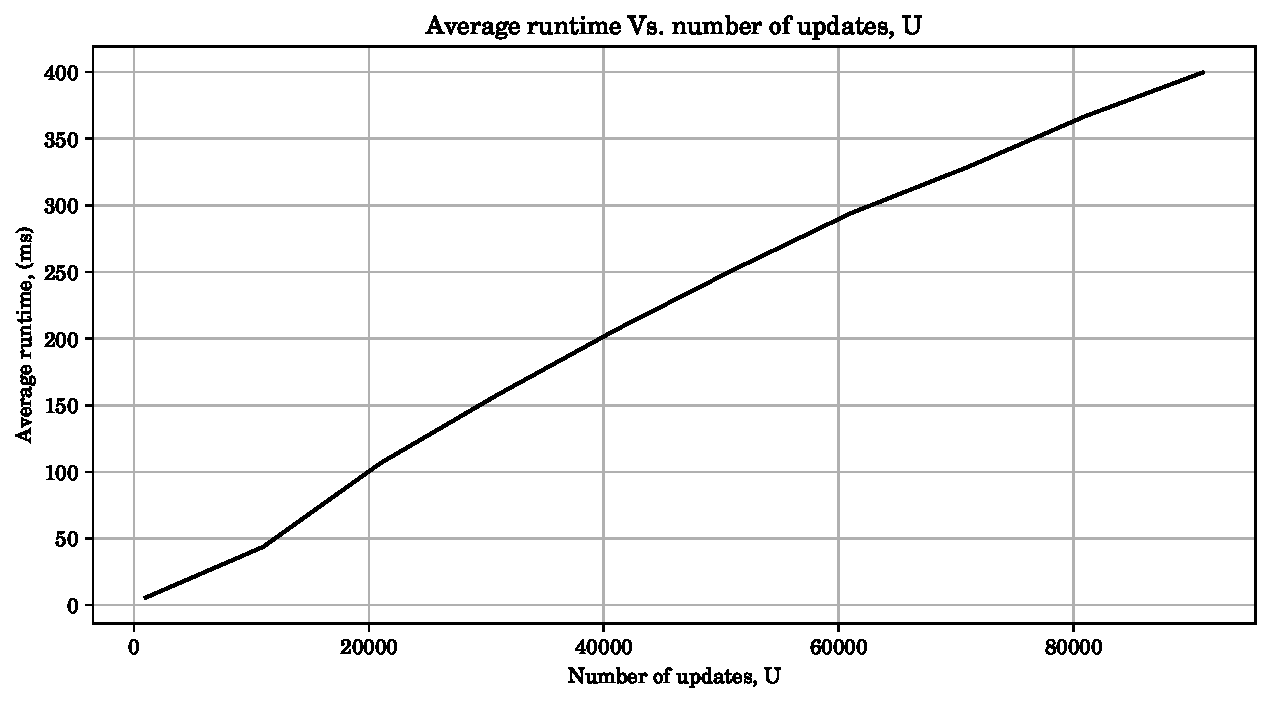
\includegraphics[width=1.0\textwidth]{./images/complexity.pdf}
    \caption{reconstruct\_orderbook runtime as a function of the number of updates, $U$.\\ Note that the runtimes are recorded 100 times and then averaged.}
    \label{complexity}
\end{figure}

\begin{figure}[htpb]
    \centering
    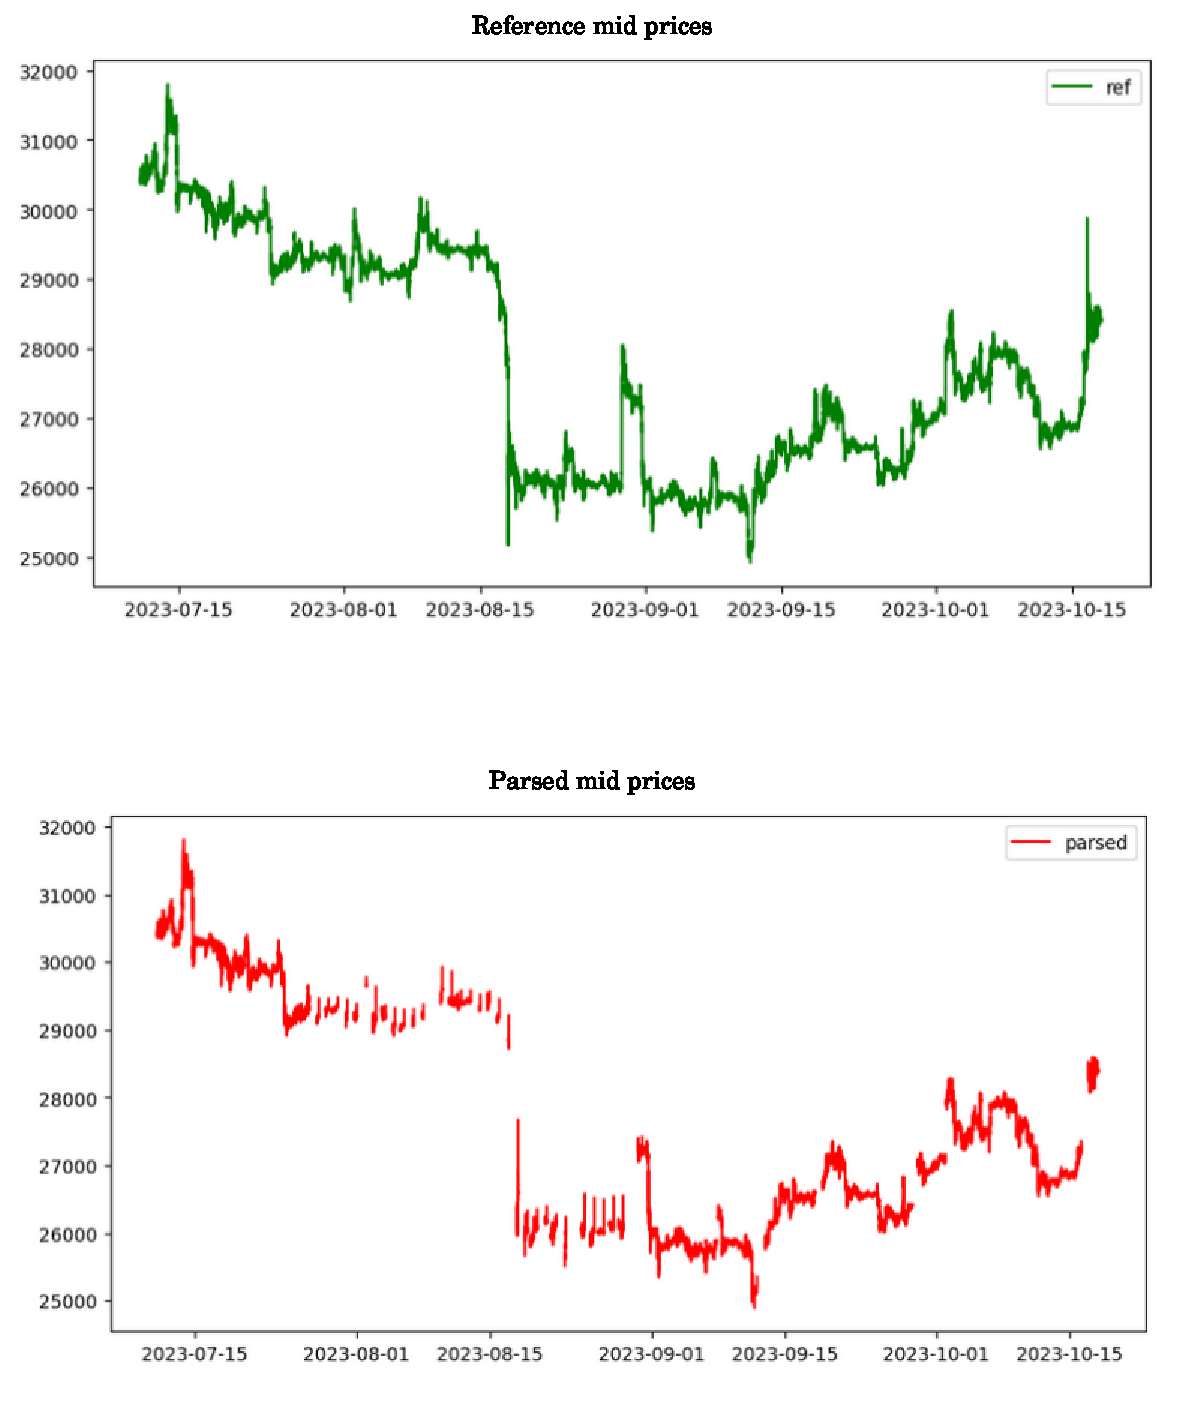
\includegraphics[width=1.0\textwidth]{./images/stitched.pdf}
    \caption{Reference hourly mid-prices (top) Vs. parsed mid-prices (bottom). Observe the general shape is correct, however
    there are large irregular gaps due to missing data.}
    \label{missing}
\end{figure}


\chapter{DeepLOB Detailed Model Architecture}

\begin{table}[ht]
        \centering
    \resizebox{0.98\textwidth}{!}{ \begin{tabular}{|l|l|l|}
                \hline
                \textbf{Layer Type} & \textbf{Parameters} & \textbf{Details} \\
                \hline
                \textbf{Conv 1} & & \\
                \quad Conv2d & $1 \times 2$, 32 filters, stride $1 \times 2$ & Spatial aggregation of price and volume for each level and side.\\
                \quad LeakyReLU & negative slope = 0.01 & Activation function.\\
                \quad BatchNorm2d & 32 features & Normalization.\\
                \quad Conv2d & $4 \times 1$, 32 filters & Temporal aggregation of price and volume for each level and side.\\
                \quad LeakyReLU & negative slope = 0.01 & \\
                \quad BatchNorm2d & 32 features & \\
                \quad Conv2d & $4 \times 1$, 32 filters & Temporal aggregation of price and volume for each level and side.\\
                \quad LeakyReLU & negative slope = 0.01 & \\
                \quad BatchNorm2d & 32 features & \\
                \hline
                \textbf{Conv 2} & & \\
                \quad Conv2d & $1 \times 2$, 32 filters, stride $1 \times 2$ & Spatial aggregation of imbalance information across sides for each level.\\
                \quad Tanh & & Activation function.\\
                \quad BatchNorm2d & 32 features & \\
                \quad Conv2d & $4 \times 1$, 32 filters & Temporal aggregation of imbalance information across time for each side and level.\\
                \quad Tanh & & \\
                \quad BatchNorm2d & 32 features & \\
                \quad Conv2d & $4 \times 1$, 32 filters & Temporal aggregation of imbalance information across time for each side and level.\\
                \quad Tanh & & \\
                \quad BatchNorm2d & 32 features & \\
                \hline
                \textbf{Conv 3} & & \\
                \quad Conv2d & $1 \times 10$, 32 filters & Spatial aggregation of imbalance information across all levels.\\
                \quad LeakyReLU & negative slope = 0.01 & \\
                \quad BatchNorm2d & 32 features & \\
                \quad Conv2d & $4 \times 1$, 32 filters & Temporal aggregation of imbalance information across all levels.\\
                \quad LeakyReLU & negative slope = 0.01 & \\
                \quad BatchNorm2d & 32 features & \\
                \quad Conv2d & $4 \times 1$, 32 filters & Temporal aggregation of imbalance information across all levels.\\
                \quad LeakyReLU & negative slope = 0.01 & \\
                \quad BatchNorm2d & 32 features & \\
                \hline
                \textbf{Inception 1} & & \\
                \quad Conv2d & $1 \times 1$, 64 filters, padding  & Increasing dimensionality.\\
                \quad LeakyReLU & negative slope = 0.01 & \\
                \quad BatchNorm2d & 64 features & \\
                \quad Conv2d & $3 \times 1$, 64 filters, padding  & Temporal aggregation simulating a moving average with window size 3.\\
                \quad LeakyReLU & negative slope = 0.01 & \\
                \quad BatchNorm2d & 64 features & \\
                \hline
                \textbf{Inception 2} & & \\
                \quad Conv2d & $1 \times 1$, 64 filters, padding  & Increasing dimensionality.\\
                \quad LeakyReLU & negative slope = 0.01 & \\
                \quad BatchNorm2d & 64 features & \\
                \quad Conv2d & $5 \times 1$, 64 filters, padding  & Temporal aggregation, simulating a moving average with window size 5.\\
                \quad LeakyReLU & negative slope = 0.01 & \\
                \quad BatchNorm2d & 64 features & \\
                \hline
                \textbf{Inception 3} & & \\
                \quad MaxPool2d & $3 \times 1$, stride $1 \times 1$, padding $(1, 0)$ & Temporal maximum.\\
                \quad Conv2d & $1 \times 1$, 64 filters, padding  & Increasing dimensionality.\\
                \quad LeakyReLU & negative slope = 0.01 & \\
                \quad BatchNorm2d & 64 features & \\
                \hline
                \textbf{LSTM Layer} & input size = 192, & Learn long term temporal features.\\
                                    & hidden size = 64, num layers = 1 & \\
                \hline
                \textbf{Fully Connected} & input size = 64, output size = 3 & Output.\\
                \hline
            \end{tabular}
    }
        \caption{DeepLOB model architecture.}
\end{table}

% \chapter{Application of the Hasbrouck Information Share}
\hrule
\vspace{40pt}

\section{The Hasbrouck Information Share}
In any market we constantly have new information/events that determine prices. This is often called "price discovery".

Price discovery is defined to be the process by which new information is incorporated into
market prices.

Suppose we have multiple price series that are based on the same underlying security, then by arbitrage these prices should not diverge significantly, since they share the same underlying stochastic factor(s).

\cite{HASBROUCK1995} refers to the shared stochastic factor as the "implicit efficient price".
This is the source of long-term permanent price change.
It assumed that each price series shares the same random walk component and that each series also has zero-mean i.i.d disturbances that are uncorrelated. 
These disturbances affect the price series movement in the short term, but often these
"innovations" will also have a permanent affect on the long term shared implicit efficient price. For example if we have BTC trading on FTX and Binance, then when the news hits
that FTX has is shutting down this will cause a temporary shock in the FTX BTC price,
that will eventually impact all other BTC markets.

The idea behind Hasbrouck's Information Share is to estimate what proportion of the long-term variance in the shared implicit efficient price can be attributed to innovations from the respective price series.

So formally, we start with a price series: $p_{t} := (p_{1t}, p_{2t}, \dots, p_{nt})^T \in \mathbb{R}^n$ where $p_{it}$ represent
individual price series which all share the same common stochastic factor (random walk component). So these series are all co-integrated $I(1)$.

\cite{HASBROUCK1995} converts this price series into a Vector Error Correction Model or VECM for short:
\begin{equation}
    \Delta p_{t} = \alpha \beta' p_{t-1} + \sum_{i=1}^k \Gamma_{i} \Delta p_{t-i} + e_{t} \in \mathbb{R}^n
\end{equation}
The first term models the long-term interaction between the different price series. The second term models the short term dynamics of each series and the final $e_{t}$ represents the innovations.

\cite{HASBROUCK1995} then re-formulates the VECM as a Vector Moving Average of VMA model:
\begin{equation}
    \Delta p_{t} = \Psi(L)e_{t} \label{VMA}
\end{equation}
This has integrated form:
\begin{equation}
    p_{t} = \Psi(1) \sum_{s=1}^t e_{s} + \Psi^*(L)e_{t}
\end{equation}
where $\Psi(L), \Psi(1), \Psi^*(L)$ are matrix polynomials in the lag operator $L$ and
\begin{equation}
    \Psi(1) = I_{n} + \sum_{t=1}^\infty \Psi_{t} \label{Psi1}
\end{equation}
So the vector $\Psi(1)e_{t}$ represents the long run impact of the innovation $e_{t}$ on each price series.

The fact that $\beta' p_{t}$ is stationary implies that $\beta' \Psi(1) = 0$ and then by construction of $\beta'$ we have that all rows of $\Psi(1)$ should be identical. In other words, we expect the long run impact
on each price series to be approximately the same. We denote the common row vector
of $\Psi(1)$ as $\psi$. So $\psi e_{t}$ gives us the component of the price change that is permanently affected by the innovation $e_{t}$. Note that:
\begin{equation}
    \text{var}(\psi e_{t}) = \psi \Omega \psi'
\end{equation}
Where we have defined $\Omega := \text{cov}(e) \in \mathbb{R}^{n \times n}$, where $e = [e_{1}; e_{2}; \dots; e_{T}]' \in \mathbb{R}^{T \times n}$
Then the variance attributed to an individual price series $j$ is given by $\psi_{j}^{2} \Omega_{jj}$ and so we arrive at the Hasbrouck Information share:
\begin{equation}
    S_{j} := \frac{\psi_{j}^{2} \Omega_{jj}}{\psi \Omega \psi'} \label{Hasequation}
\end{equation}
However as \cite{HASBROUCK1995} points out, if the innovations are not un-correlated across price series, then $\Omega$ will not be diagonal and this measure won't make sense.

So the Cholesky decomposition is used to try and alleviate the contemporary correlations.
Decompose $\Omega$ as:
\begin{equation}
    \Omega = F F'
\end{equation}
where $F$ is a lower triangular matrix. Then we can attain an upper/lower bound on the
information share $j$ when the price series $j$ is first/last in $p_{t}$, with:
\begin{equation}
    S_{j} = \frac{([\psi F]_{j})^{2}}{\psi \Omega \psi'}
\end{equation}

To estimate $\Psi(1)$, we turn to the work of \cite{KARABIYIK2022} who derive the following estimators:

\begin{align}
\beta' &:= [1_{(n-1)}; -I_{(n-1)}] \in \mathbb{R}^{(n-1) \times n} \\
\hat{\alpha} &:= \Delta p' M_{x} p_{-1}^* [ (p_{-1}^*)' M_{x} p_{-1}^*]^{-1} \in \mathbb{R}^{n \times (n-1)}\\
\Delta p &:= [\Delta p_{1}; \dots ; \Delta p_{T}]' \in \mathbb{R}^{T \times n} \\ 
p_{-1}^* &:= [\beta' p_{0}; \dots ; \beta' p_{T-1}]' \in \mathbb{R}^{T \times (n-1)} \\
&= [p_{0}; \dots ; p_{T-1}]' \beta \\
M_{x} &:= I_{T} - X(X'X)^{-1} X' \in \mathbb{R}^{T \times T} \\
X &:= [\Delta p_{-k}; \dots ; \Delta p_{-1}] \in \mathbb{R}^{T \times kn} \\
\Delta p_{-l} &:= [\Delta p_{1-l}; \dots ; \Delta p_{T-l}]' \in \mathbb{R}^{T \times n} \\
\hat{e} &:= M_{x}(\Delta p - p^{*}_{-1} \hat{\alpha}') \in \mathbb{R}^{T \times n}\\
\hat{\Omega} &:= \frac{1}{T} \hat{e}' \hat{e} \in \mathbb{R}^{n \times n}
\end{align}

Then they also derive a consistent estimator for $\alpha_{\perp} \in \mathbb{R}^{n \times 1}$ by taking the only eigenvector of $M_{\hat{\alpha}} := I_{n} - \hat{\alpha}(\hat{\alpha}' \hat{\alpha})^{-1} \hat{\alpha}'$ with eigenvalue $1$. (Normalized to have norm $1$).
Following \cite{HASBROUCK1995}, they also take the Cholesky decomposition of $\hat{\Omega}$ to get $\hat{F}$.
(We refer the interested reader to \cite{KARABIYIK2022} for derivation and proofs of these estimators).

So using these estimators we arrive at an estimator for the information share of the $j^{th}$ price series:

\begin{equation}
    \hat{IS}_{j} := \frac{([ \hat{\alpha}_{\perp}'\hat{F}]_{j})^2}{\hat{\alpha}_{\perp}' \hat{\Omega} \hat{\alpha}_{\perp}}
\end{equation}

As \cite{HASBROUCK1995} points out, the ordering of the price series will have an effect on the information share, so to achieve upper/lower bounds on information share for price series $j$, we permute the $p$ so that the $p_{j, t}$ is first/last.


\section{A Toy Example}
We demonstrate this methodology with a synthetic example.

Suppose we have two price series, with the first being modelled as a simple random walk
and the second modelled as a lagged version of the first, with some extra randomness introduced.

\begin{align}
    p_{1, t} &= p_{1, t-1} + w_{1, t} = w_{1, t} + w_{1, t-1} + \sum_{s=1}^{t-2} w_{1, s} \label{toy1}\\
    p_{2, t} &= p_{1, t-2} + w_{2, t} = w_{2, t} + \sum_{s=1}^{t-2} w_{1, s} \label{toy2}
\end{align}

Where $w_{j, t} \sim N(0, 1)$ i.i.d and $p_0 := 0$.

We can clearly verify that this example is co-integrated $I(1)$.

This could represent two different markets, each with their own news shocks/innovations
where the second market reacts to the first market price changes. So in this
situation we would have an information share of $1$ for the first market and $0$ for the
second market, since the first market completely drives price discovery.

\begin{figure*}[htpb]
    \centering
    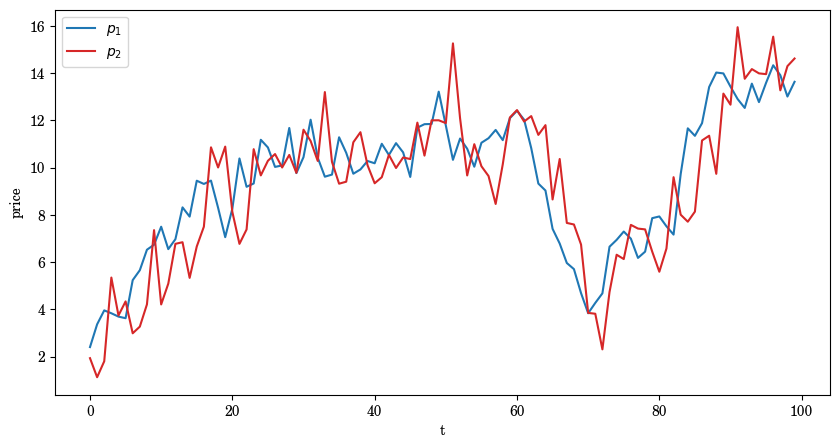
\includegraphics[width=1.0\textwidth]{./images/lagged_walk.png}
    \caption{Lagged random walks. Clearly we see $p_2$ lags behind $p_1$. Note that we only plot $t$ up to 100 for visual clarity.}
\end{figure*}

We derive this result analytically in the following.

Using (\ref{toy1}) and (\ref{toy2}) we get:
\begin{align*}
    \Delta p_{1, t} &= w_{1, t} \\
    \Delta p_{2, t} &= w_{1, t-2} + w_{2, t} - w_{2, t-1}
\end{align*}

Then we can convert to the VMA representation given in (\ref{VMA}):
\[
    \underbrace{
    \begin{bmatrix}
    w_{1,t} \\
    w_{1,t-2} + w_{2,t} - w_{2,t-1}
    \end{bmatrix} 
    }_{= \Delta p}
    =
    \underbrace{
    \begin{bmatrix}
    1 & 0 \\
    L^{2}  & 1 - L
    \end{bmatrix}
    }_{= \Psi(L)}
    \underbrace{
    \begin{bmatrix}
    w_{1,t} \\
    w_{2,t}
    \end{bmatrix}
    }_{=e_t}
.\]

Then recalling that $\Psi(L) = \sum_{k=0}^{\infty} \Psi_k L^k$ 
we have the coefficients:
\begin{align*}
    \Psi(L) =
\underbrace{
\begin{bmatrix}
1 & 0 \\
0 & 1
\end{bmatrix}
}_{:= \Psi_0} L^0
+
\underbrace{
\begin{bmatrix}
0 & 0 \\
0 & -1
\end{bmatrix}
}_{:= \Psi_1} L^1
+
\underbrace{
\begin{bmatrix}
0 & 0  \\
1 & 0
\end{bmatrix}
}_{:= \Psi_2}L^{2}
\end{align*}
Then plugging these into (\ref{Psi1}) we get:
\[
    \Psi(1) = \begin{bmatrix} 1 & 0 \\ 1 & 0 \end{bmatrix} 
.\]
Which has common row vector $\psi := [1 ~ 0]$. Then using (\ref{Hasequation})
and $\Omega = I_2$ we get the Information Share of the first price series to be $1$
and the Information Share of the second series to be $0$, as expected.

% We also examine the case when we have two simple random walks:
%
% \begin{align}
%     p_{1, t} &= p_{1, t-1} + w_{1, t} = \sum_{s=1}^{t} wShare{1, s}\\
%     p_{2, t} &= p_{2, t-1} + w_{2, t} = \sum_{s=1}^{t} w_{2, s}
% \end{align}
%
% \textbf{TODO:} Analytically derive hasbrouck information share for this example.
%
% Where $w_{j, t} \sim N(0, 1)$ i.i.d and $p_0 := 0$.
%
% Clearly this example is co-integrated $I(1)$, since $\mathbb{E}(p_{j,t}) = \sum_{s=1}^{t} \mathbb{E}(w_{j,s}) = 0$ and
% $\text{var}(p_{j, t}) = \sum_{s=1}^{t} \text{var}(w_{j, s}) = t$
% and therefore $\mathbb{E}(\Delta p_t) = \text{var}(\Delta p_t) = 0$.
%
%
% \begin{figure}[htpb]
%     \centering
%     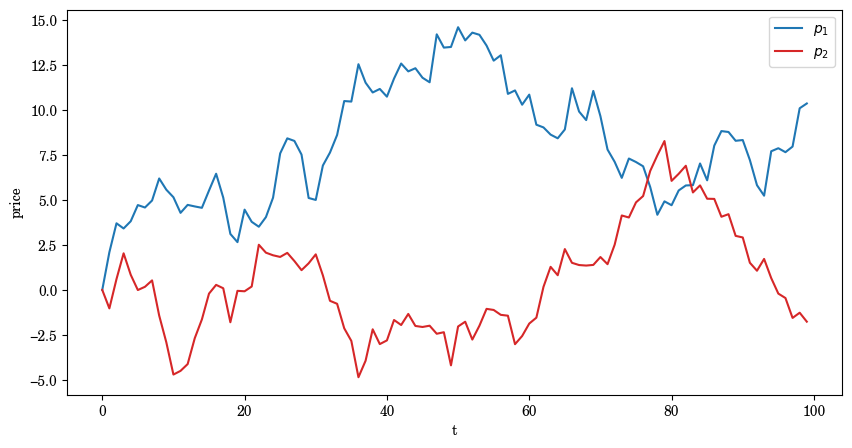
\includegraphics[width=1.0\textwidth]{./images/random_walk.png}
%     \caption{Random walks}
% \end{figure}
%
\section{Orderbook Application}

Following \cite{CAO2009} we resample our data to $1s$ intervals and define the weighted price as:
\begin{equation}
    \text{WP}^{n_{1}, n_{2}} := \frac{\sum_{j=n_{1}}^{n_{2}} q_{j}^B p_{j}^B + q_{j}^A p_{j}^A}{\sum_{j=n_{1}}^{n_{2}} (q^B_{j} + q^A_{j})}
\end{equation}
where $n_{1} \leq n_{2}$. When $n_{1} = n_{2} = 1$ we have the weighted mid-price:
\begin{equation}
    \text{WP}^{1,1} = \frac{q_{1}^B p_{1}^B + q_{1}^A p_{1}^A}{q_{1}^B + q_{1}^A}
\end{equation}

So $\text{WP}^{n_{1},n_{2}}$ is an average price between level $n_{1}$ and $n_{2}$, weighted by volume, encapsulating all the information in the orderbook between levels $n_{1}$ and $n_{2}$ inclusive.

We compare the information content of $\text{WP}^{1,1}$ and $\text{WP}^{2,10}$, i.e how does the information
at the top of the book compare to the other, deeper levels.
So our price series is given by $p_t := (\text{WP}^{1,1}_t, \text{WP}^{2,10}_t)$.
The mid-price and the weighted price have the same common stochastic factor,
are both non-stationary and therefore it is clear that they are $I(1)$ co-integrated.

\begin{figure*}[htpb]
    \centering
    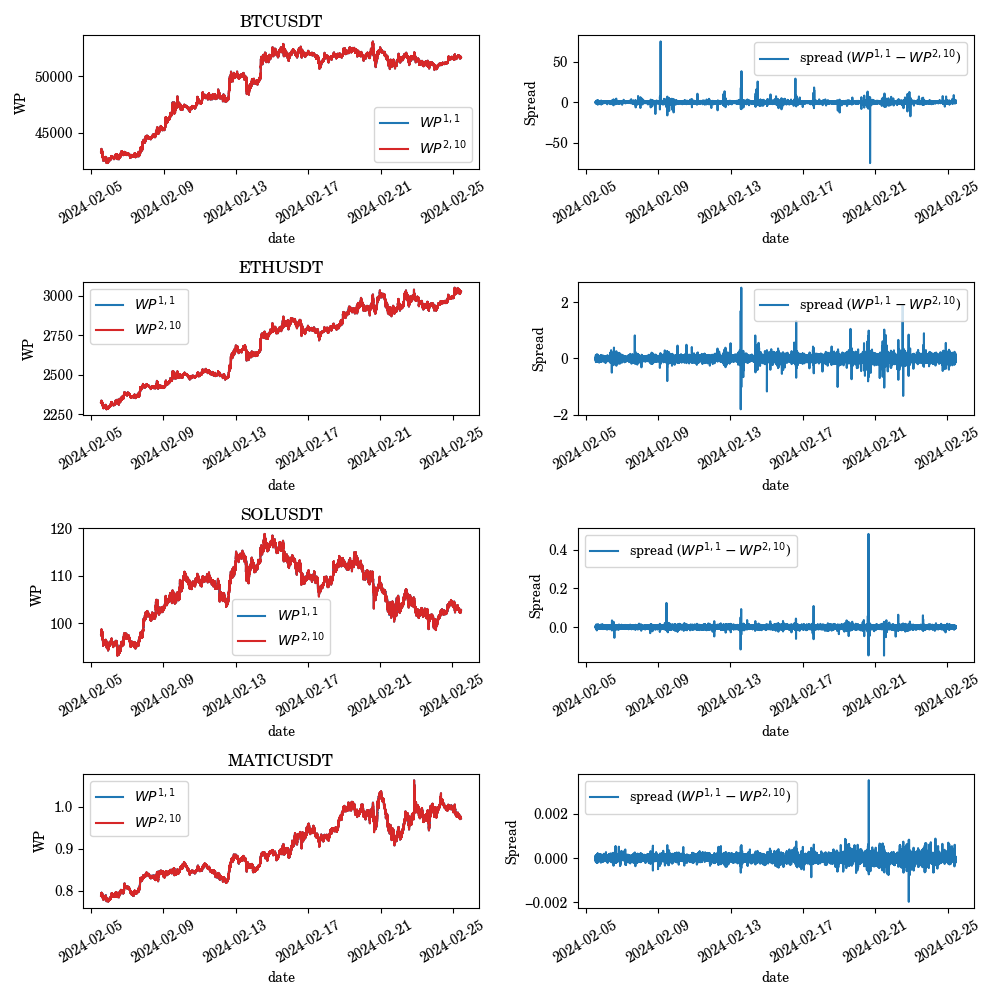
\includegraphics[width=1.0\textwidth]{./images/weighted_prices.png}
    \caption{Weighted prices and their spread for each trading pair.}
    \label{spread}
\end{figure*}

Interestingly we see from Figure \ref{spread} that for our data BTCUSDT
has some very large outlier spreads whereas MATICUSDT seems to be much more stable.
Also we observe that in general across all our trading pairs there is a slight increase
in spread towards the end of the month.


So now we calculate \footnote{Note that when calculating information shares, we have too much data to fit
into memory, so we calculate the information share for windows of size 10,000 and then
we average. Standard deviations are also given in parenthesis.} the Information Share using the estimators we defined above
and report the results in Table \ref{table:1}.

\begin{table}[H]
    \begin{center}
        \begin{tabular}{ccccc}
            \toprule
            trading pair    & $\text{WP}^{1,1}$ Min IS & $\text{WP}^{1,1}$ Max IS & $\text{WP}^{2,10}$ Min IS & $\text{WP}^{2,10}$ Max IS \\
            \midrule
            BTCUSDT   & 0.05 (0.04)  & 0.97 (0.02)   & 0.03 (0.02) & 0.95 (0.04)   \\
            ETHUSDT   & 0.06 (0.05)  & 0.98 (0.03)   & 0.02 (0.03) & 0.94 (0.05)  \\
            SOLUSDT   & 0.08 (0.05)     & 0.98 (0.02)  & 0.02 (0.02) & 0.92 (0.05)   \\
            MATICUSDT &   0.04 (0.06)    & 0.87 (0.12)  & 0.13 (0.12) & 0.96 (0.06)  \\
            \bottomrule
        \end{tabular}
        \caption{IS Results for each trading pair.}
    \label{table:1}
    \end{center}
\end{table}

So we see that for each price series the minimum IS is close to zero and the maximum is close 1.
This is unexpected. For example when \cite{CAO2009} applied the same methodology they
had a much tighter spread between max and min information share for each stock.
This large difference means that for us information share is hard to interpret and 
is perhaps not as useful for this application as one would have hoped.
As \cite{YAN2010} points out, large differences in minimum and maximum Information Share
occur when the residuals, $e_t$ are highly correlated across series.

When we examine our estimated $\Omega$ covariance matrices we find this to be the case.
This implies that the innovations at the top of the orderbook are highly correlated
with the innovations affecting prices further down the orderbook. As \cite{KARABIYIK2022}
points out, these correlations can be partly alleviated by using higher frequency data.
We re-sample our data to 250ms intervals (instead of 1s) and observe a reduction
in covariance. However this reduction is not sufficient and we still observe a large gap in max and min Information Shares.
This is perhaps due to the fact that
for cryptocurrency data the trading is much higher volume and higher frequency
than traditional stocks as studied in \cite{CAO2009}, and so in order for the 
innovations to be uncorrelated, we need much higher frequency sampling.
Since we are limited by our Websocket data to a minimum resolution, we can go no further. 

We conclude that for Binance Websocket data, information shocks
driving price change are highly correlated across orderbook levels.
A consequence of this being that the Hasbrouck Information Share cannot be applied reliably
to measure Information Shares across levels.



%%%%%%%%%%%%%%%%%%%%%%%%%%%%%%%%%%%%%
\bibliography{bibliography.bib}
%%%%%%%%%%%%%%%%%%%%%%%%%%%%%%%%%%%%%

\end{document}
